% This is file orientation-sedimentation.tex
% first release v1.0, 20th October 1996
%       release v1.01, 29th October 1996
%       release v1.1, 25th June 1997
%       release v2.0, 27th July 2004
%       release v3.0, 16th July 2014
%   (based on JFMsampl.tex v1.3 for LaTeX2.09)
% Copyright (C) 1996, 1997, 2014 Cambridge University Press

\documentclass[]{jfm}

\usepackage{dcolumn}% Align table columns on decimal point
\usepackage{bm}% bold math
\usepackage{color,soul}
%\usepackage{enumerate}
%\usepackage{hyperref}% add hypertext capabilities

\usepackage{graphicx}
\usepackage{epstopdf, epsfig}
\usepackage{amsmath}
\usepackage{amssymb}

\newtheorem{lemma}{Lemma}
\newtheorem{corollary}{Corollary}

\shorttitle{Orientation and Sedimentation}
\shortauthor{S. Kramel, U. Menon, D. L. Koch and G. A. Voth}

\title{Orientation and Sedimentation of Ramified Particles in Turbulence}

\author{S. Kramel\aff{1}, U. Menon\aff{2}, D. L. Koch\aff{2} \and G. A. Voth\aff{1}
	\corresp{\email{gvoth@wesleyan.edu}}
	}

\affiliation{\aff{1}Department of Physics, Wesleyan University, Middletown, Connecticut 06459, USA
\aff{2}Department of Chemical and Biomolecular Engineering, Cornell University, Ithaca, NY 14853, USA}

\begin{document}

\maketitle

\begin{abstract}
The orientation distribution of non-spherical particles plays a fundamental role in understanding cloud micro physics, optical phenomena and in improving remote sensing applications. In this study, we present experimental measurements of orientation distributions and sedimentation statistics of ramified particles, settling under gravity and various levels of turbulence.
\end{abstract}

\begin{keywords}
Authors should not enter keywords on the manuscript, as these must be chosen by the author during the online submission process and will then be added during the typesetting process
\end{keywords}

Outline: \\

\begin{enumerate}
	\item{Introduction} \\
	Introduce ramified particles; \\
	\item{Experiments} \\
	Apparatus; Jet Array; Data Acquisition; Particles; Parameter Space; Particle Suspension; Settling number; \\
	\item{Theory} \\
	Need to add description of theoretical model and simulation methods. Simple ramified particle model (SRPM) for fibers and triads using mobility tensor approach.  \\
	\item{Results} \\
	\begin{enumerate}
		\item{Quiescent Fluid} \\
		Show results from quiescent fluid experiments and SRPM. \\
		\item{Turbulence} \\
		Show orientation PDFs and sedimentation statistics \\
	\end{enumerate}
	\item{Conclusions} \\
\end{enumerate}

\section{Introduction}
The orientation of non-spherical particles sedimenting in turbulence plays an important role in [...] and cloud micro physics, optical phenomena and remote sensing. \\

Following the introduction of \cite{2013Siewert} Simulations of orientation and settling velocity of ellipsoids in decaying turbulence: \\
\begin{enumerate}[I]
\item Influence of turbulence in clouds on formation of precipitation (\cite{2012Devenish})
\item Collision probabilities, collision kernels and the modification of the collision kernel by modifying the relative particle velocity (\cite{2010Beheng},\cite{2013Grabowski})
\item Little known about the mixed phase of droplets and ice particles (\cite{1998Pinsky}) due to complicated shape (\cite{1997Pruppacher})
\item Strong alignment of non-spherical particles turbulence is unable to destroy (\cite{1981Cho})
\item In agreement with orientation model of \cite{1995Klett}
\item Measurements of ellipsoids in quiescent fluid (\cite{1994Newsom}). With increasing turbulence, preferential orientation decreases (\cite{1988Krushkal},\cite{1998Newsom})
\item Many literature on fibers without inertia (\cite{2005Parsheh},\cite{2005Shin},\cite{2009Wilkinson},\cite{2011Parsa},\cite{2011Pumir},\cite{2012Parsa})
\item Presence of inertia introduces new effects: enhanced sedimentation for inertial spheres (\cite{1993Wang})
\item Time scale that particles need to reach stable orientation is larger than the turbulent time scale, therefore Lagrangian simulation of ellipsoids in turbulence is required (\cite{2012Gavze})\\
\end{enumerate} 

From \cite{2014Hashino}:\\
\begin{enumerate}[I]
\item Implication for remote sensing (\cite{2011Westbrook}), origin of Perry Arc
\item Specular reflection of hexagonal plates is observed with lidar in ice clouds from earth (\cite{2002Noel},\cite{2010Westbrook}) and space \cite{2007Hu}.
\item Well known that ice crystals do knot fall straight but the motion depends on the Reynolds number and the dimensionless moment of inertia \cite{1964Willmarth}, \cite{1972Zikmunda}, \cite{1997Field} and \cite{1992Kajikawa}\\
\end{enumerate}

Structure of the paper: Introduction; Experiments: Apparatus, particles, parameter space; Orientation PDFs; Theory and more Results: sedimentation statistics; Conclusions;

\newpage

\section{Experiments}
APPARATUS--  We constructed a 14 ft. (4.2 m) tall, vertical water tunnel (see Fig. \ref{Fig:watertunnel}a) to keep heavy particles suspended and simultaneously control the amount of turbulence they experience.  The particles are being suspended by a laminar through flow, which keeps them in the test section and allows us to record long, individual trajectories.  To ensure a flat velocity profile of the through flow, the fluid first passes through a pressure plate (2\% open area), a 20 cm tall honeycomb flow straightener and a contraction zone (area ratio 4:1) before entering the test section.  The exit conditions downstream of the test section are kept symmetric to the inlet conditions.  It is a recirculating system and the fluid is carefully degassed to eliminate air bubbles. The temperature is monitored and relatively stable around the room temperature of $24.5^{\circ}$C.  One of the challenges of the experiments is keeping the particles suspended without clogging filters, valves or the pump.

JET ARRAY-- Turbulence is generated and controlled with a jet-array, a 3d-printed passive grid (using Nylon and Selective Laser Sintering, grid spacing $M=6$ cm, 30\% solidity) with internal channels and 40 nozzles (see Fig. \ref{Fig:watertunnel}b).  Each nozzle can be triggered independently through a solenoid valve and eject a jet of fluid into the surrounding flow.  In the minimum turbulence configuration, all valves are closed and the jet-array generates decaying turbulence typical of a passive grid, with low turbulence intensities.  The system can also be driven solely through the jet-array, similar to the random jet-array used by \cite{2008Variano}, achieving much larger turbulence intensities.  The intermediate turbulence regimes can be reached by either adjusting the number of jets, the duration each jet is firing or the jet velocity.  The generated turbulence is very isotropic in the horizontal plane, but has a larger rms fluctuating velocity in the vertical direction (the direction of the through flow), as shown in table \ref{tab:kd1}.  Both, through flow and jet-array are powered by a 3 hp, variable speed pump that can produce a through flow of up to 10 cm/s in the test section and an estimated jet velocity of up to 4 m/s at the nozzles. 
\begin{figure}
\centering
  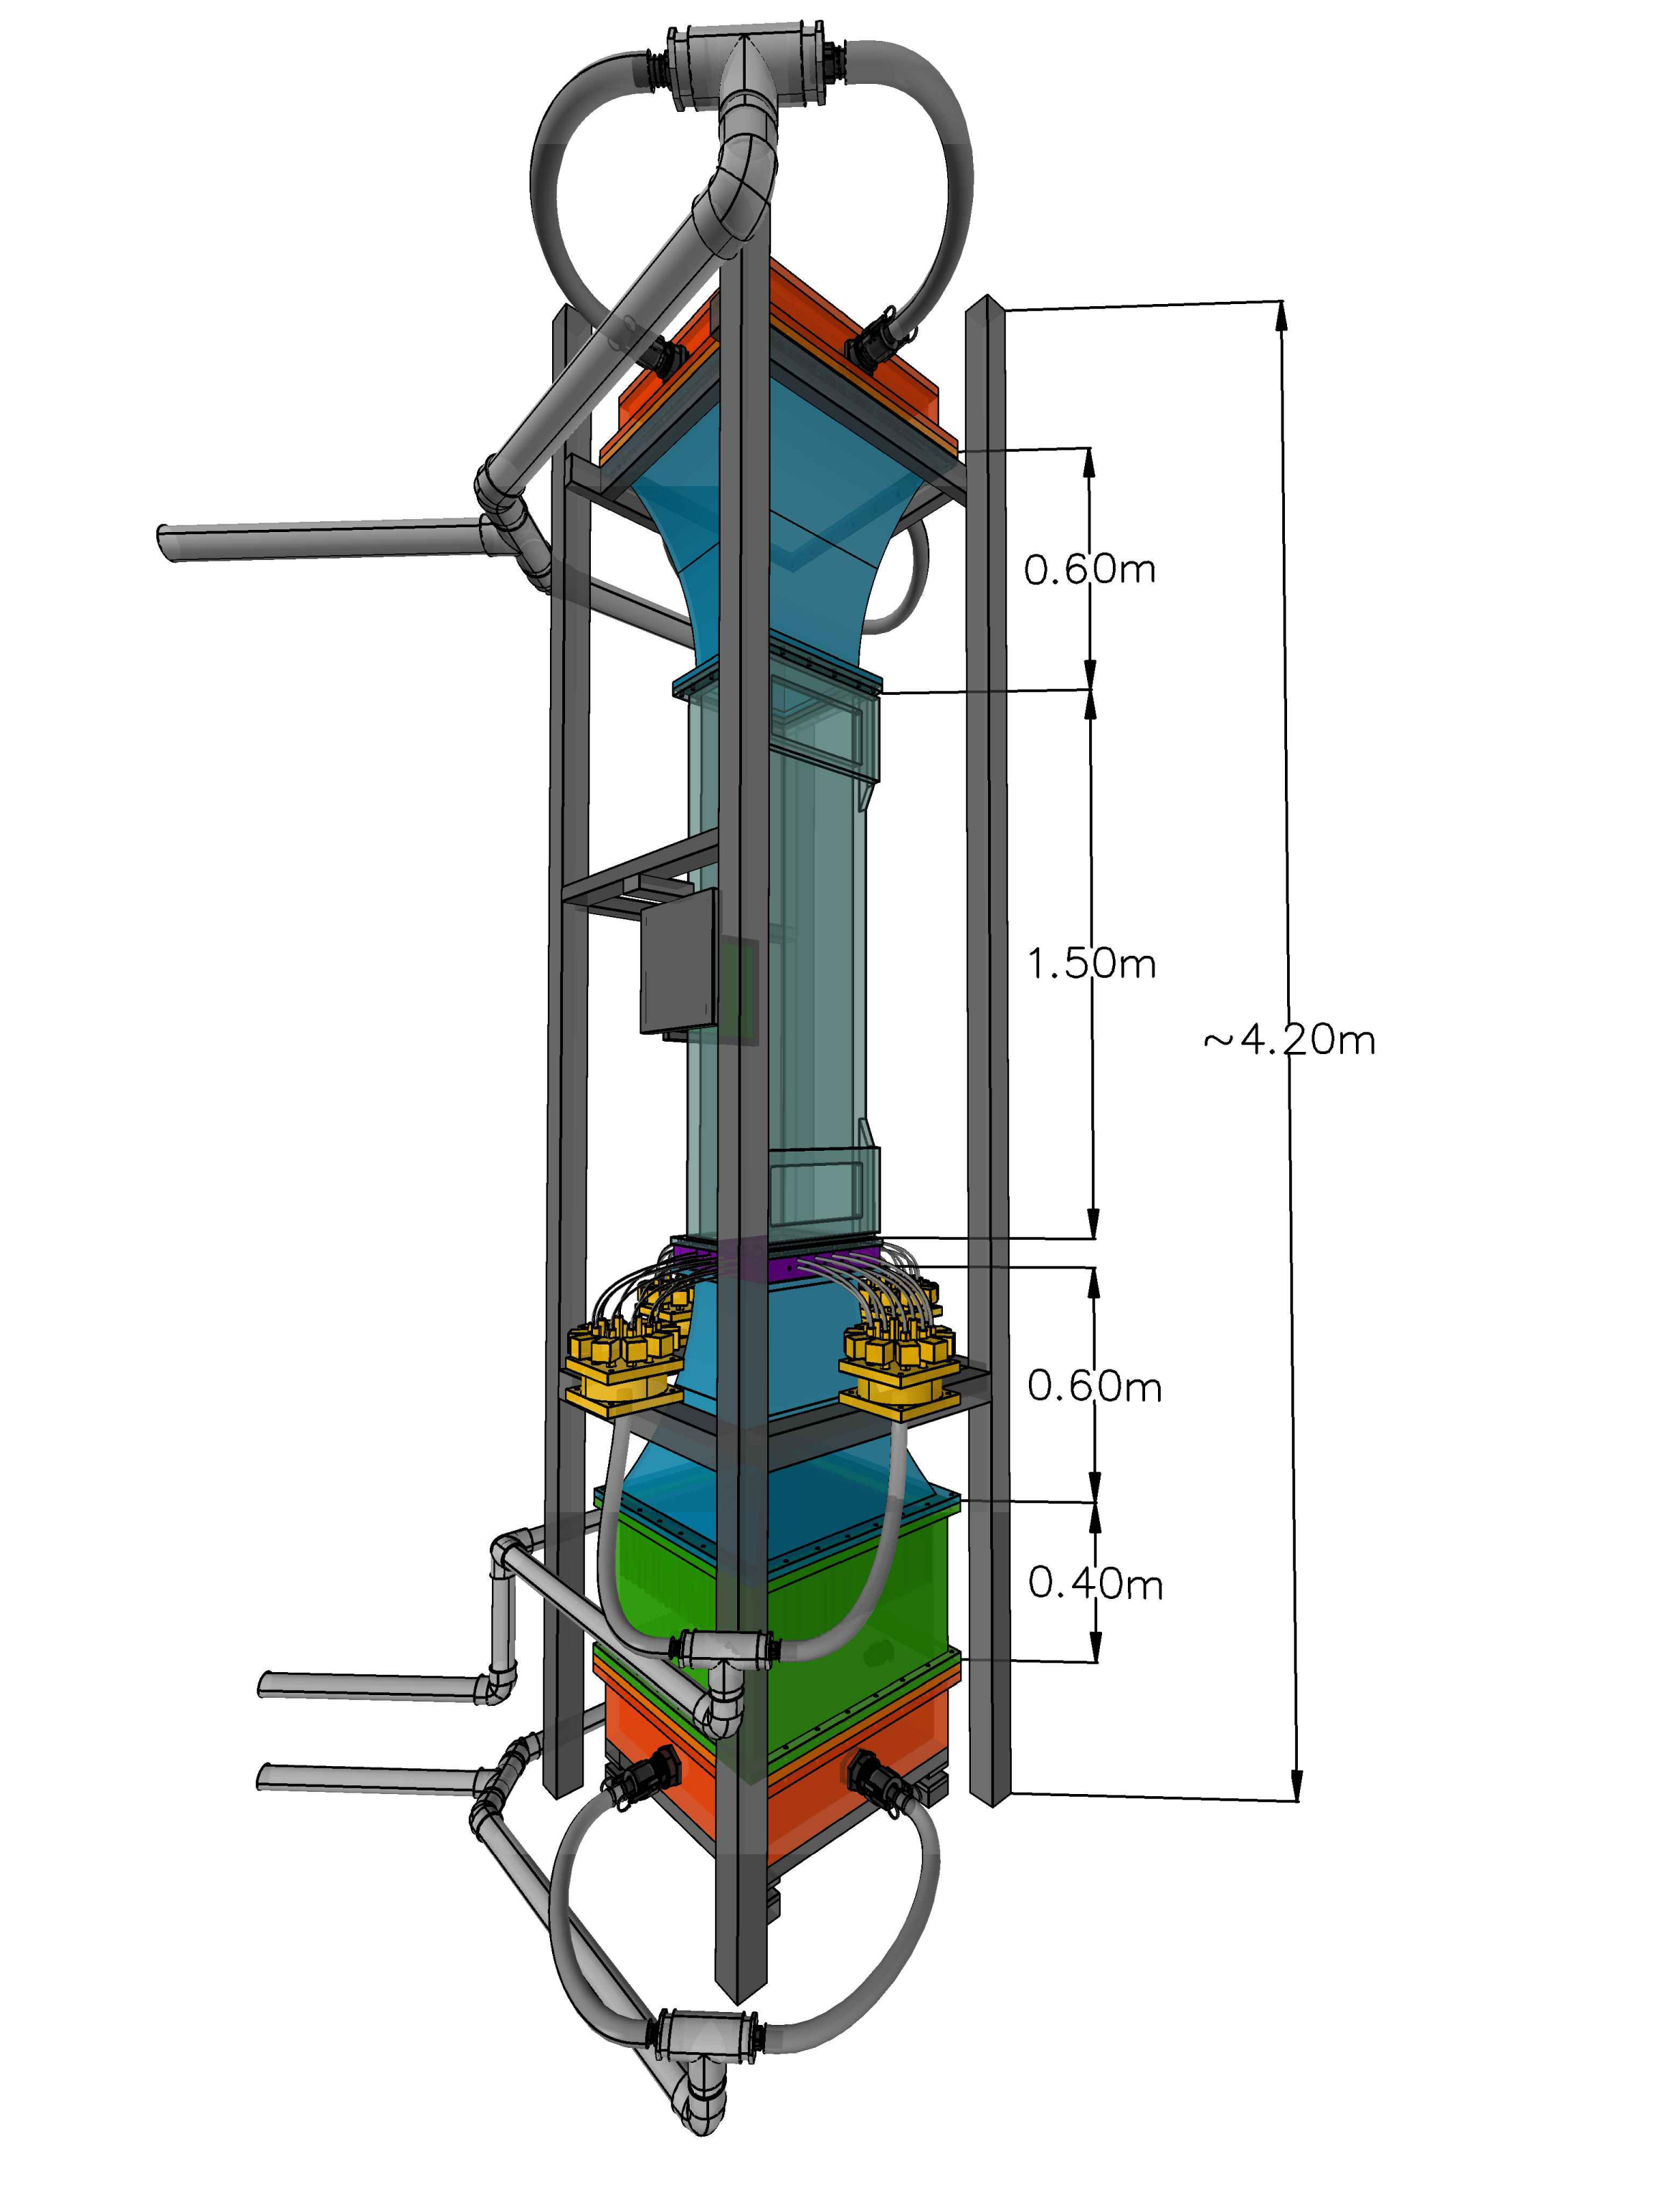
\includegraphics[width=5.5in]{figures/watertunnel.pdf}
  \caption{a) Autocad rendering of the vertical water tunnel. From bottom to top (color online): inlet chamber for through flow (orange), pressure plate and honeycomb (green), contraction zone (blue), manifolds (yellow) for jet array (purple), test section (clear), expansion zone (blue), flow exit chamber (orange). b) 3d-model of the active jet array. c) Side view of a slice through the jet array shows internal channels, turning vanes and nozzles.}
	\label{Fig:watertunnel}
\end{figure}

DATA ACQUISITION-- Two coarse meshes confine the particles in a clear, 30 x 30 x 150 cm$^3$ tall test section, where four high speed cameras image a $12$ x $12$ x $10$ cm$^3$ detection volume in the center region, 10$M$ downstream of the jet-array.  Two high powered, pulsed and monochromatic LED lights (SmartVisionLights ODMOBL series) create a uniform background illumination.  The cameras and the lights are triggered synchronously at 450 Hz, ensuring a single pulse illumination during each exposure.  A real-time image compression system, which allows continuous data acquisition for several days, is used to collect enough data.  It is essential for these experiments, because there is not always a particle view, let alone on all four cameras, which is required to determine an accurate particle orientation.

PARTICLES--  The particles used in the experiments are also 3d-printed (using VeroBlack material and Fused Deposition Modeling, $\rho_p=1.143$ g cm$^{-3}$) and consist of several slender fibers, connected at the center (we call them ramified particles).  In this case, three fibers of equal length $l'$ and radius $r$ with aspect ratio $\kappa=l'/r=10$, oriented in planar symmetry and with a 120$^{\circ}$ angle between them, form a triad (see Fig. \ref{Fig:triad}).  A triad is used as a model particle for oblate spheroids (disks) with equivalent aspect ratio of $\kappa=l/d$, where $l=2l'$ and $d=2r$ (crosses are expected to show equivalent statistics).  The advantage of using ramified particles as models is that the orientation can be measured much more accurately and even rotations within the plane of the disk can be resolved easily.  

We fabricated roughly 150 particles with smallest dimension $r=225$ $\mu$m (referred to as small triads, but not Stokes small) and 150 particles with $r=450$ $\mu$m (large particles), both with $\kappa=20$.  The particle Reynolds number $\textit{Re}_d = wd/\nu$ based on the fiber diameter ranges from $\textit{Re}_d=10$ to $\textit{Re}_d=40$ (see Table~\ref{tab:kd3}), where $w$ is the relative particle velocity and $\nu=0.9131 \times 10^{-6}$ m$^{2}$ s$^{-1}$ is the fluid viscosity.  Grey, neutrally buoyant micro spheres with a diameter of 250 $\mu$m were used as tracer particles to measure the fluid velocity, calculate structure functions and extract mean energy dissipation rates $\epsilon$. 

PARAMETER SPACE-- Inertial particles sedimenting in turbulence cover a wide range of parameters that need to be explored and characterized.  A dimensional analysis of the problem yields five dimensionless groups, which can be used to describe non-spherical particles sedimenting in turbulence. The aspect ratio $\kappa$, describing the particle shape and the density ratio $\Delta \rho= \rho_p/\rho_f$ of particle and fluid causing inertial effects are already two dimensionless quantities.  The Reynolds number $\textit{Re}_{\lambda}=\sqrt{15\bar{u}L/\nu}$ and the non-dimensional particle size $l/\eta$, where $\eta$ is the Kolmogorov length, connecting the particle scale with the turbulent length scale, are two more.  We define the last dimensionless quantity to be the settling number $S_F$.  It relates fluid inertia and gravity, similar to the Froude number $\textit{Fr}=\sqrt{lg}/\bar{u}$, however, in this case the settling number is used as a measure of the inertial torques acting on the particles.  The analytical expression for $S_F{=}\frac{5}{8\log{2\kappa}}(\frac{w}{u_{\eta}})^2$ is derived later and is compared to an empirical $S_F=\tau_l/\tau_{\textit{inert}}$, measured in separate experiments. 

With these five parameters in mind, we chose six different turbulence intensities for the experiments, ranging from $S_F\ll1$, where we expect weak inertial effects and randomly oriented particles, to $S_F\gg1$, where inertial torques dominate the the particles are strongly aligned with their preferential orientation direction.  The particle shape and density ratio, $\kappa$ and $\Delta \rho$, were fixed in the experiments and therefore the inertial torques acting on the particles was nearly constant.  $S_F$ was varied by adjusting the turbulence intensities in the detection volume.  The amount of turbulence can be controlled by the the jet velocity of the jet array.  The number of jets firing at the same time was fixed to 8 (20\% of the total number of jets), the average duration of a jet was set to 1 s ($\pm$0.25 s) and jets were chosen randomly with some restrictions for neighboring jets.  A summary of the parameters for all experiments can be seen in Table \ref{tab:kd3}

\begin{table}
  \begin{center}
\def~{\hphantom{0}}
  \begin{tabular}{cccccc} 
      $\textit{Re}_{\lambda}$ & $l/\eta$ & $S_F$ & $\kappa$ &$\Delta \rho$ & ($\textit{Re}_d$) \\[3pt]

			34 (35) & 4.5 (14.3) & 6.36 (5.49) & 20 & 1.146 & 10.82 (35.74) \\
			95 (56) & 9 (14.3) & 2.39 (4.95) & 20 & 1.146 & 11.06 (35.26) \\
			141 (102) & 16.9 (32.1) & 0.99 (1.84) & 20 & 1.146 & 11.88 (36.89) \\
			162 (153) & 23.0 (45) & 0.70  (1.05) & 20 & 1.146 & 12.31 (40.34) \\
			192 (162) & 25.7 (51) & 0.58  (0.94) & 20 & 1.146 & 12.36 (39.58) \\
      194 (200) & 27.3 (72) & 0.55 (0.64) & 20 & 1.146 & 12.21 (33.25) \\	 

  \end{tabular}
  \caption{Non-dimensional parameters used to describe sedimentation of small (large) triads.  $\textit{Re}_{\lambda}{=}\sqrt{15\bar{u}L/\nu}$, Reynolds number;  $l/\eta$, non-dimensional particle size (small triads: $l=9$ mm, large triads: $l=18$ mm);  $S_F{=}\tau_l/\tau_{\textit{inert}}$, settling number; $\tau_l{=}\sqrt{4/15} (2l/u_l^T)$, turbulence response time at the scale of the particle; $u_l^T$, magnitude of the second-order transverse velocity structure function at scale $l$, $\tau_{\textit{inert}}$, characteristic time for a particle to return to its equilibrium position due to inertial torques (measured experimentally in quiescent fluid); $\kappa=l/r$, aspect ratio; $\Delta \rho=\rho_p/\rho_f$, density ratio. $\textit{Re}_d$, particle Reynolds number based on the diameter (additional non-dimensional parameter).  }
  \label{tab:kd3}
  \end{center}
\end{table}

PARTICLE SUSPENSION--  The particles have to be suspended near the center of the test section in order to take continuous data and gather enough statistics. Depending on particle size, the through flow can be adjusted to match their sedimentation rate in quiescent fluid.  As we increase the turbulence intensity, triads start to rotate around their equilibrium sedimentation orientation which, in return, increases their sedimentation rate.  The through flow was adjusted to keep as many triads suspended as possible.  For the highest turbulence intensities, triads were almost entirely suspended by strong jets from the jet array, whereas for intermediate turbulence intensities, the through flow had to be increased. triads in the lowest turbulence intensity show the same orientation and sedimentation statistics as triads in quiescent fluid.  The absolute fluid velocities for through flow and through the jet array were measure with two separate magnetic flow meters (Toshiba GF630 series).  The measured values are listed in table \ref{tab:kd4}

\begin{table}
  \begin{center}
\def~{\hphantom{0}}
  \begin{tabular}{cccccc}
			Small triads \\
			\hline
			Turb. Int. & Thru flow & Total jet flow & Pump Speed & $ u_f $ ($\sigma$) & $ u_p $ ($\sigma$) \\
			0.08 & 1.7 & 0 & 700 & 19.78 (0.94) & -2.93 (1.32) \\
			0.23 & 1.3 & 0.4 & 800 & 23.39 (4.13) & -0.09 (5.01) \\
			0.39 & 1.4 & 1.0 & 1200 & 29.85 (9.84) & 5.38 (11.33) \\
			0.62 & 0.9 & 1.5 & 1550 & 26.91 (14.52) & 2.56 (17.03) \\
			0.91 & 0.2 & 2.1 & 2000 & 21.96 (16.40) & -2.69 (19.78) \\
      1.06 & 0 & 2.2 & 2100 & 20.08 (17.08) & -4.70 (20.16) \\
			\hline 
			Large triads \\
			\hline
			Turb. Int. & Thru flow & Total jet flow & Pump Speed & $ U_f $ ($\sigma$) & $ u_p $ ($\sigma$) \\
			0.07 & 2.9 & 0 & 1150 & 34.14 (2.52) & -1.65 (2.98) \\
			0.10 & 2.1 & 0.3 & 900 & 30.63 (3.08) & -5.12 (3.35) \\
			0.29 & 1.6 & 0.8 & 1100 & 31.68 (9.16) & -6.61 (8.2) \\
			0.28 & 3.2 & 1.0 & 1700 & 58.00 (15.99) & 16.35 (14.43) \\
			0.37 & 2.5 & 1.3 & 1700 & 50.29 (18.73) & 8.80 (16.98) \\
      0.95 & 0.6 & 2.5 & 2500 & 30.06 (28.42) & -3.95 (30.28) \\
			\\
  \end{tabular}
  \caption{Additional Flow parameters: Total jet flow through 8 nozzles with an average firing time of 1 second (std = .25 s), $U_f$ was measured with tracer particles, $\sigma = (\langle U_f^2\rangle - \langle U_f \rangle^2)^{1/2}$}
  \label{tab:kd4}
  \end{center}
\end{table}

SETTLING NUMBER-- The settling number $S_F$ (subscript: F for fibers, T for triads) is a measure of the ratio of particle rotation rate due to inertial torques and turbulence.  In the experiments, this number can be quantified empirically as the ratio of particle response time $\tau_{\textit{inert}}$ over the turbulent time scale of the fluid at the size of the particle $\tau_l$.  The particle response time $\tau_{\textit{inert}}$ was measured in separate experiments, in quiescent fluid, as the characteristic time for the particle to return to its equilibrium orientation and $\tau_l = \sqrt{4/15}~(l/u_l^T)$, where $u_l^T$ is the magnitude of the second-order transverse velocity structure function at scale $l$. 

\section{Theory}

\section{Results}
\subsection{Quiescent Fluid}

QUIESCENT FLUID-- In addition to a drag force, non-spherical particles like fibers and disks have a non-zero horizontal settling velocity, a lift force is acting on them.  Figure~\ref{Fig:particle-velocity} shows the components of the relative particle velocity $\mathbf{w}$ as function of $p_z$ for fibers (blue circles) and triads (red triangles).  The top curves show the vertical component of $\mathbf{w}$, in the direction of gravity, $w_z$.  Fibers sediment two times faster in their vertical orientation, i.e. $w_z(p_z{=}1)=2w_z(p_z{=}0)$, whereas for triads, $w_z(p_z{=}0)=1.4w_z(p_z{=}1)$.  In Stokes flow, there is also one orientation for which fibers, spheres and disks of equal mass will sediment with the same vertical velocity.  This occurs at $p_z\approx 0.57$ ($32^{\circ}$). One has to keep in mind that $\mathbf{p}$ points along the long axis of the fiber, but is perpendicular to the plane of a disk.  Theoretically, triads should sediment 1.5 times faster when $p_z{=}0$ compared to $p_z{=}1$, however, this is not observed.  Reasons for a lower value are finite particle Reynolds number and finite aspect ratio effects, as well as the interaction between individual fibers, which doesn't exist for actual disks.  

The bottom curves show the horizontal component of $\mathbf{w}$, in the plane of $\mathbf{p}$ and gravity, $w_y$. Fibers have a larger horizontal velocity than disks for all orientations. Independent of shape, the maximum horizontal velocity is reached at $p_z = 1/\sqrt{2}$ ($45^{\circ}$). At this angle, the model predicts that fibers have $2$ times the horizontal velocity of triads.  The experiments show that both, fibers and triads, reach the largest horizontal velocity at a much lower angle, when $p_z=0.5$ (fibers: $30^{\circ}$ with the horizontal, triads: $60^{\circ}$ between the plane of the disk and the horizontal).  It should be noted that the shallowest trajectory occurs at a different angle.  

\begin{figure}
\centering
  \includegraphics[width=3.8in]{figures/model-data-comparison.pdf}
  \caption{Components of the relative particle velocity $\mathbf{w}$ as function of particle orientation, $p_z$, normalized by the mobility when $\mathbf{p}\parallel\mathbf{w}$, $M_{\parallel}$.  Top curves show the vertical component of $\mathbf{w}$.  Solid lines show the model prediction (see Appendix B) for infinitely thin disks with $M_{\parallel}{=}2M_{\perp}$ (dashed lines: $M_{\parallel}{=}1.9M_{\perp}$ and finite aspect-ratio).  Dashed-dotted lines show the model prediction for infinitely long fibers with $M_{\parallel}{=}2M_{\perp}$.  Circles and triangles represent measurements of fibers and triads in quiescent fluid.}
	\label{Fig:particle-velocity}
\end{figure}

%\begin{figure}
  %\includegraphics[width=5.5in]{figures/aspect-ratio.pdf}
  %\caption{Ratio of parallel and perpendicular mobility as function of aspect ratio. The dotted lines show the dependence on the ratio of parallel and perpendicular mobility for each fiber.}
%\label{Fig:aspect-ratio}
%\end{figure}

\subsection{Turbulence}

A triad is one of the simplest realizations of a ramified particle to model an oblate spheroid (disk).  From triads to Crosses, with an increasing number of fibers, a disk is reached in the limit of many fibers.  Using slender body theory, it can be shown that triads (as well as Crosses) mimic disks and are indeed good models to use.  The orientation of a disk is described by the unit vector $\mathbf{p}$ along the particles symmetry axis.  

In quiescent fluid and in equilibrium, triads sediment with $p_z=1$, where the z component of $\mathbf{p}$ is parallel to the direction of gravity.  This is a stable sedimentation orientation, meaning there are no torques acting on the particle. An unstable sedimentation orientation for triads is when $p_z=0$. Again, there are no torques acting on the particle, however, a small perturbation is enough and the particle rotates toward the stable orientation.  The triads used in the experiments can not be considered small and the interactions between individual fibers of a triad can not be neglected.  These effects appear in particle specific deviations from the disk limit, e.g. triads show a second stable orientation within the plane of the disk (add figure?).  

ORIENTATION-PDFs-- Figure \ref{Fig:orientation-PDF} shows how the probablity density function (PDF) of $p_z$ changes as the turbulence intensity changes.  The colormap indicates increasing turbulence intensities (or decreasing $S_F$), from blue/cold to red/hot, respectively.  For the lowest turbulence intensities (blue curves), small triads (Fig.~\ref{Fig:orientation-PDF} left) and large triads (Fig.~\ref{Fig:orientation-PDF} right) are strongly aligned with the direction of gravity within a few degrees.  As we increase the turbulence intensity, the orientation PDFs become wider, approaching the random orientation distribution (black dashed line).  Even for the largest jet velocity needed to fully randomize the particle orientation underestimated the inertial torques and we can still see some alignment, even in the most turbulent cases (red curves).  It should be noted that the orientation PDFs of small and large particles should not be directly compared.  Due to the different sedimentation rate of small and large particles, the through flow and the jet velocity had to be adjusted.  If the statistics had been know ahead of time, one could have aimed for the same non-dimensional parameters in the experiments and more specifically looked at the effects of particle size.  

\begin{figure}
\centering
\begin{minipage}{.5\textwidth}
  \centering
  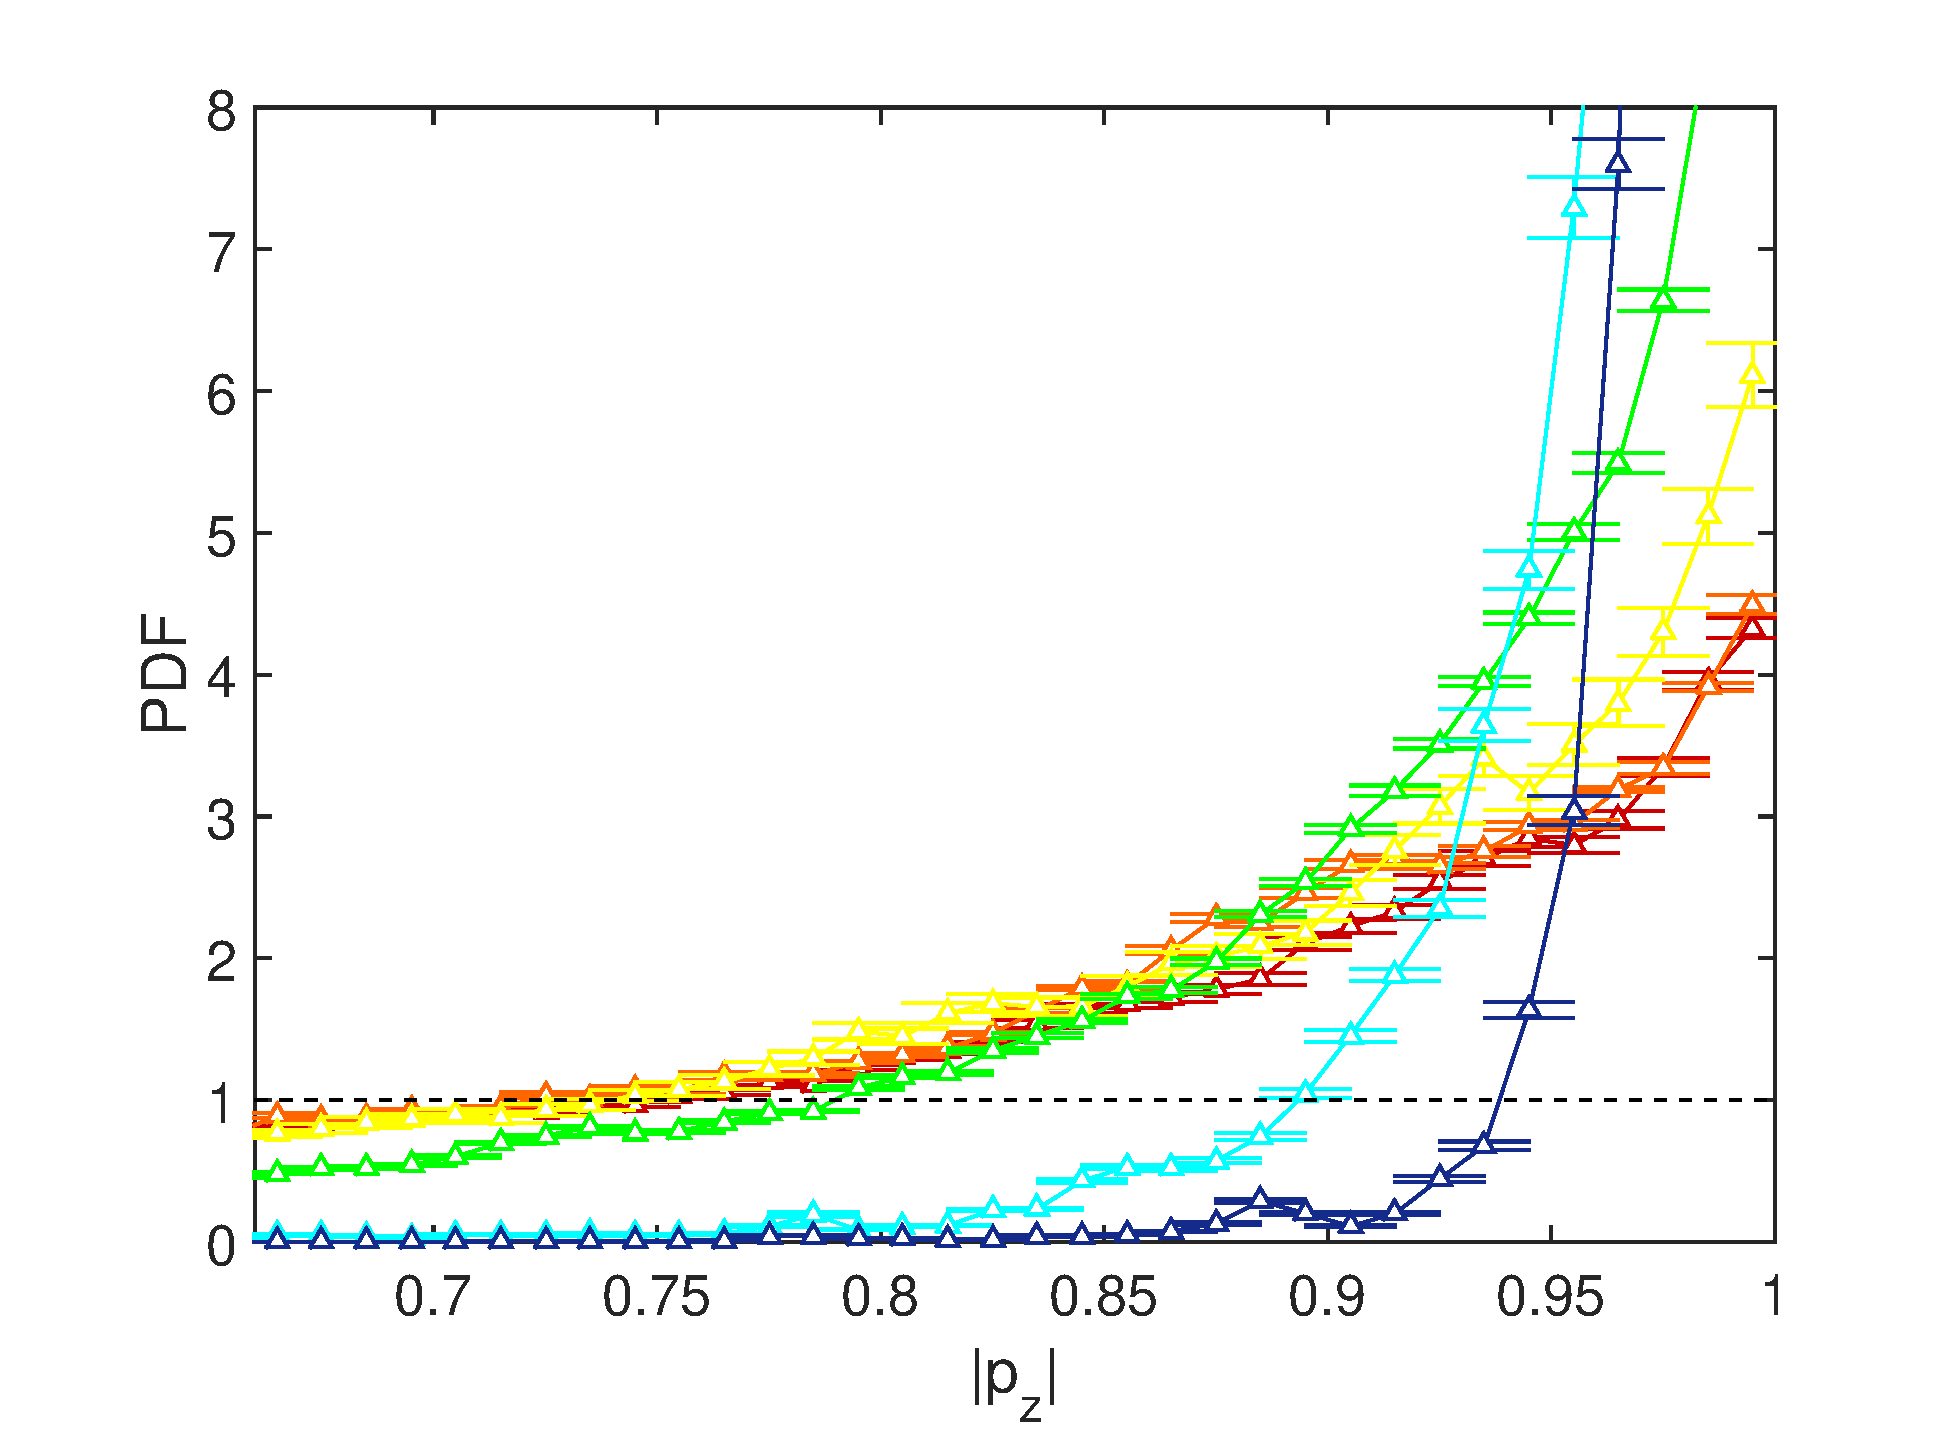
\includegraphics[width=2.9in]{figures/orientation-PDF-small.pdf}
\end{minipage}%
\begin{minipage}{.5\textwidth}
  \centering
  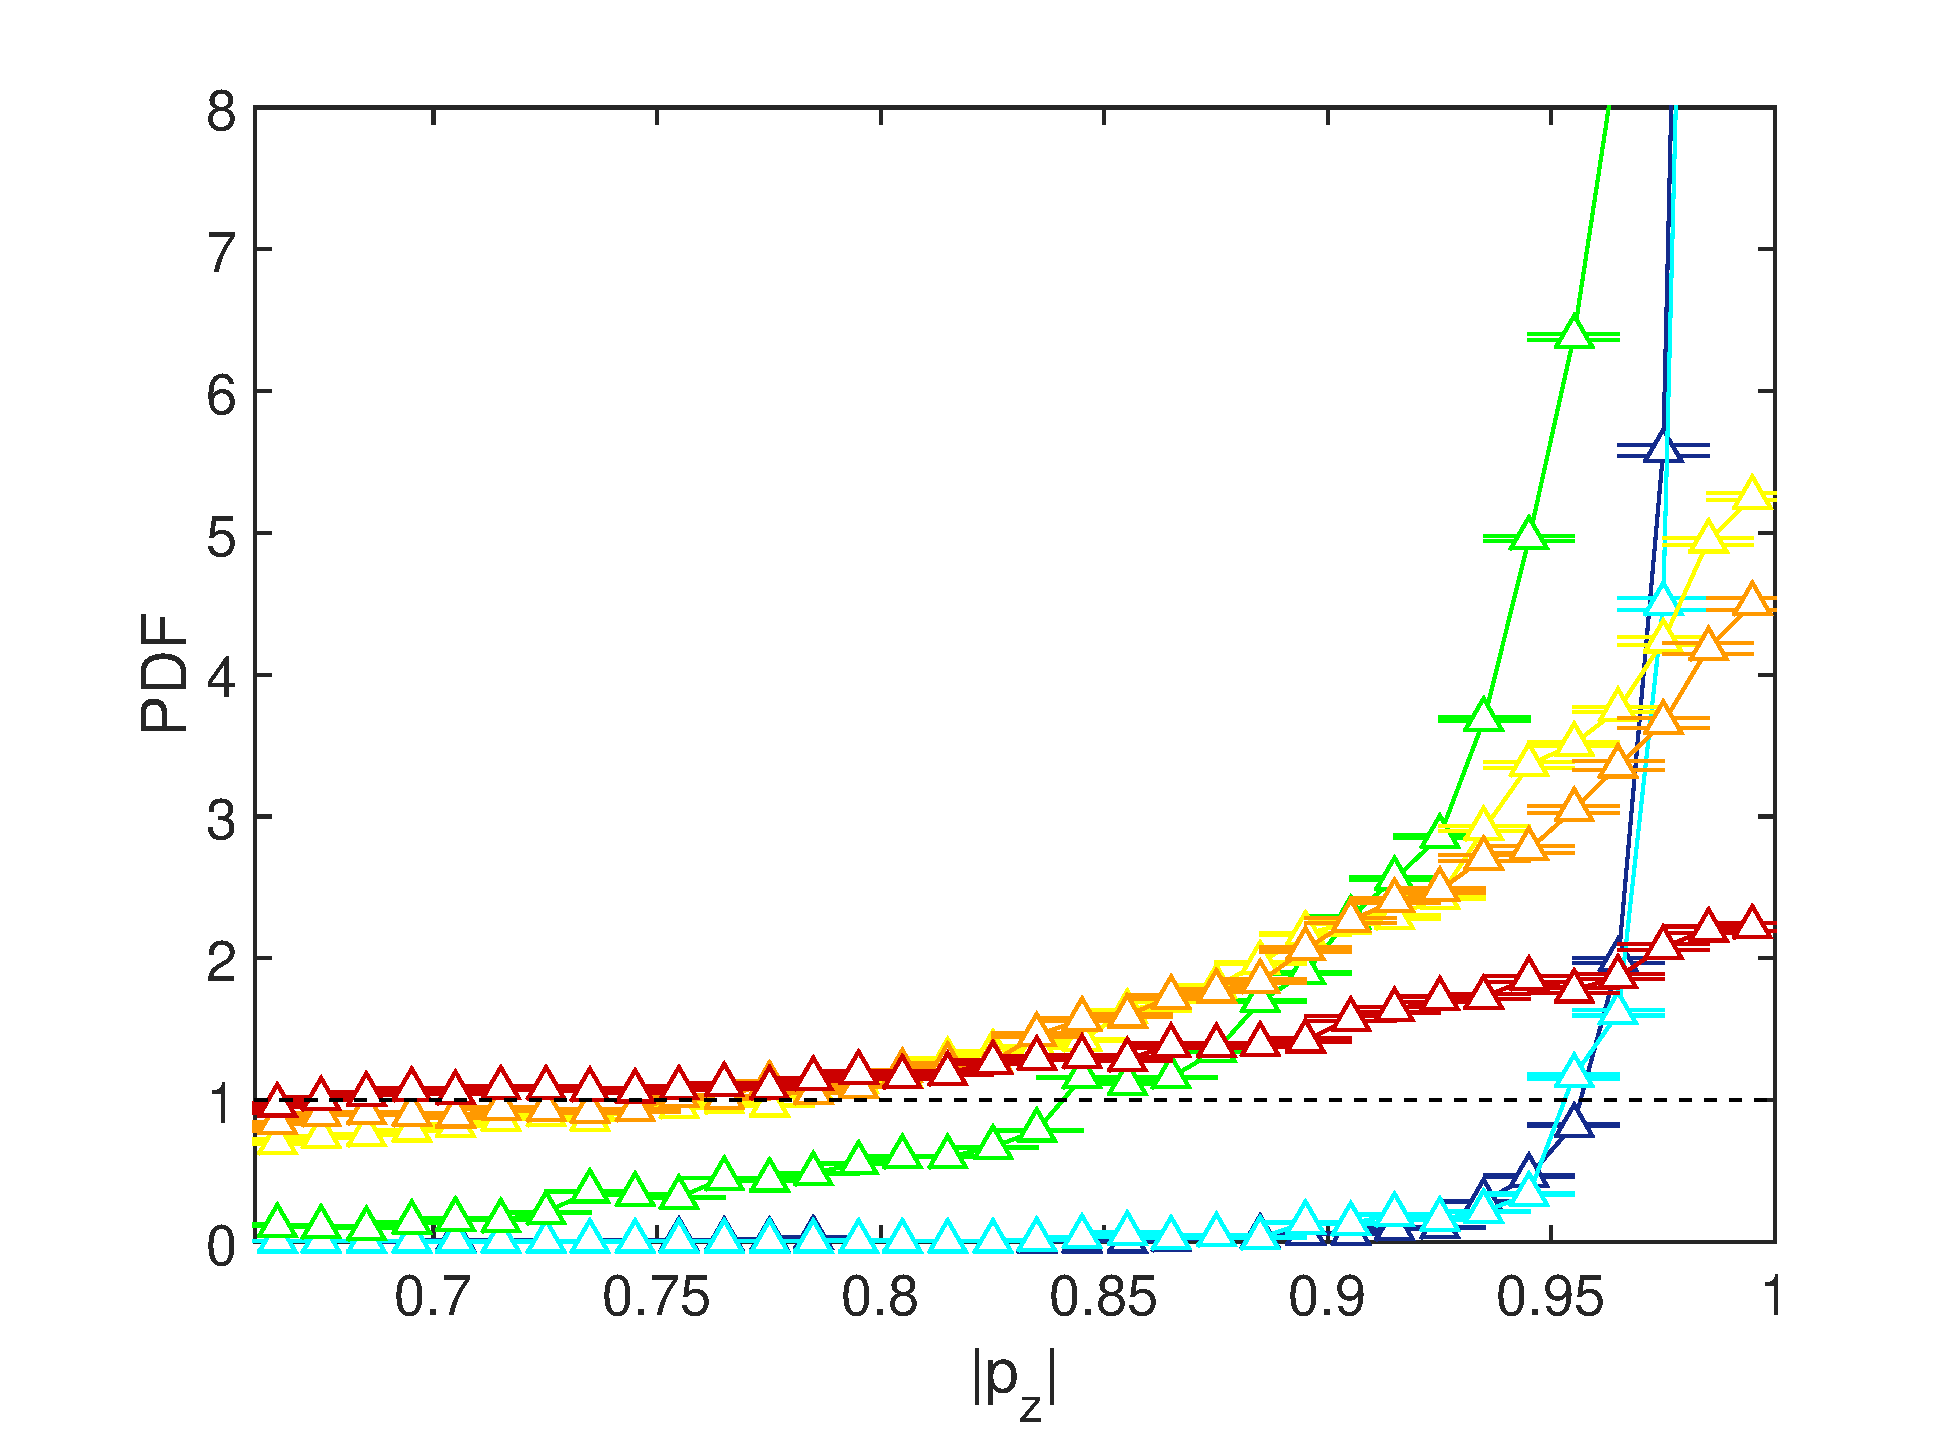
\includegraphics[width=2.9in]{figures/orientation-PDF-large.pdf}
\end{minipage}

\caption{Orientation Probability Distribution Function (PDF) for small (left) and large (right) triads. The colormap indicates turbulence intensities, from red (most turbulent) to blue (least turbulent). For the lowest Reynolds number, particles are oriented within less than 3$^{\circ}$ of the direction of gravity. For the largest Reynolds number, particle orientations are almost randomly distributed. Errorbars represent the standard error. }
\label{Fig:orientation-PDF}
\end{figure}

SETTLING NUMBER-- Figure~\ref{Fig:mean-square} shows the mean square of the components of $\hat{p}$ as function of settling number.  For $S_F\ll1$, triads approach random orientations where $\langle p_i^2 \rangle = 1/3$.  With increasing $S_F$, turbulence intensity decreases and the inertial torques become more dominant causing triads to approach the strongly aligned limit for which $\langle p_z^2 \rangle \rightarrow 1$ and $\langle p_{(x,y)}^2 \rangle \rightarrow 0$.  Theoretically, fibers approach this strongly aligned limit according to a power law proportional to $S_F^{-2}$.  The data suggests that this is also true for triads.  For the largest value of $S_F$, particle inhomogeneities caused by fabrication defects set a lower limit for reliable $\langle p_i^2 \rangle$ measurements in the experiments, explaining the larger than predicted $\langle p_{(x,y)}^2 \rangle$ of the small triads.  Figure~\ref{Fig:mean-square} shows measurements of $\langle p_i^2 \rangle$ in quiescent fluid as comparison, dashed lines.  

\begin{figure}
\centering
\begin{minipage}{.5\textwidth}
  \centering
  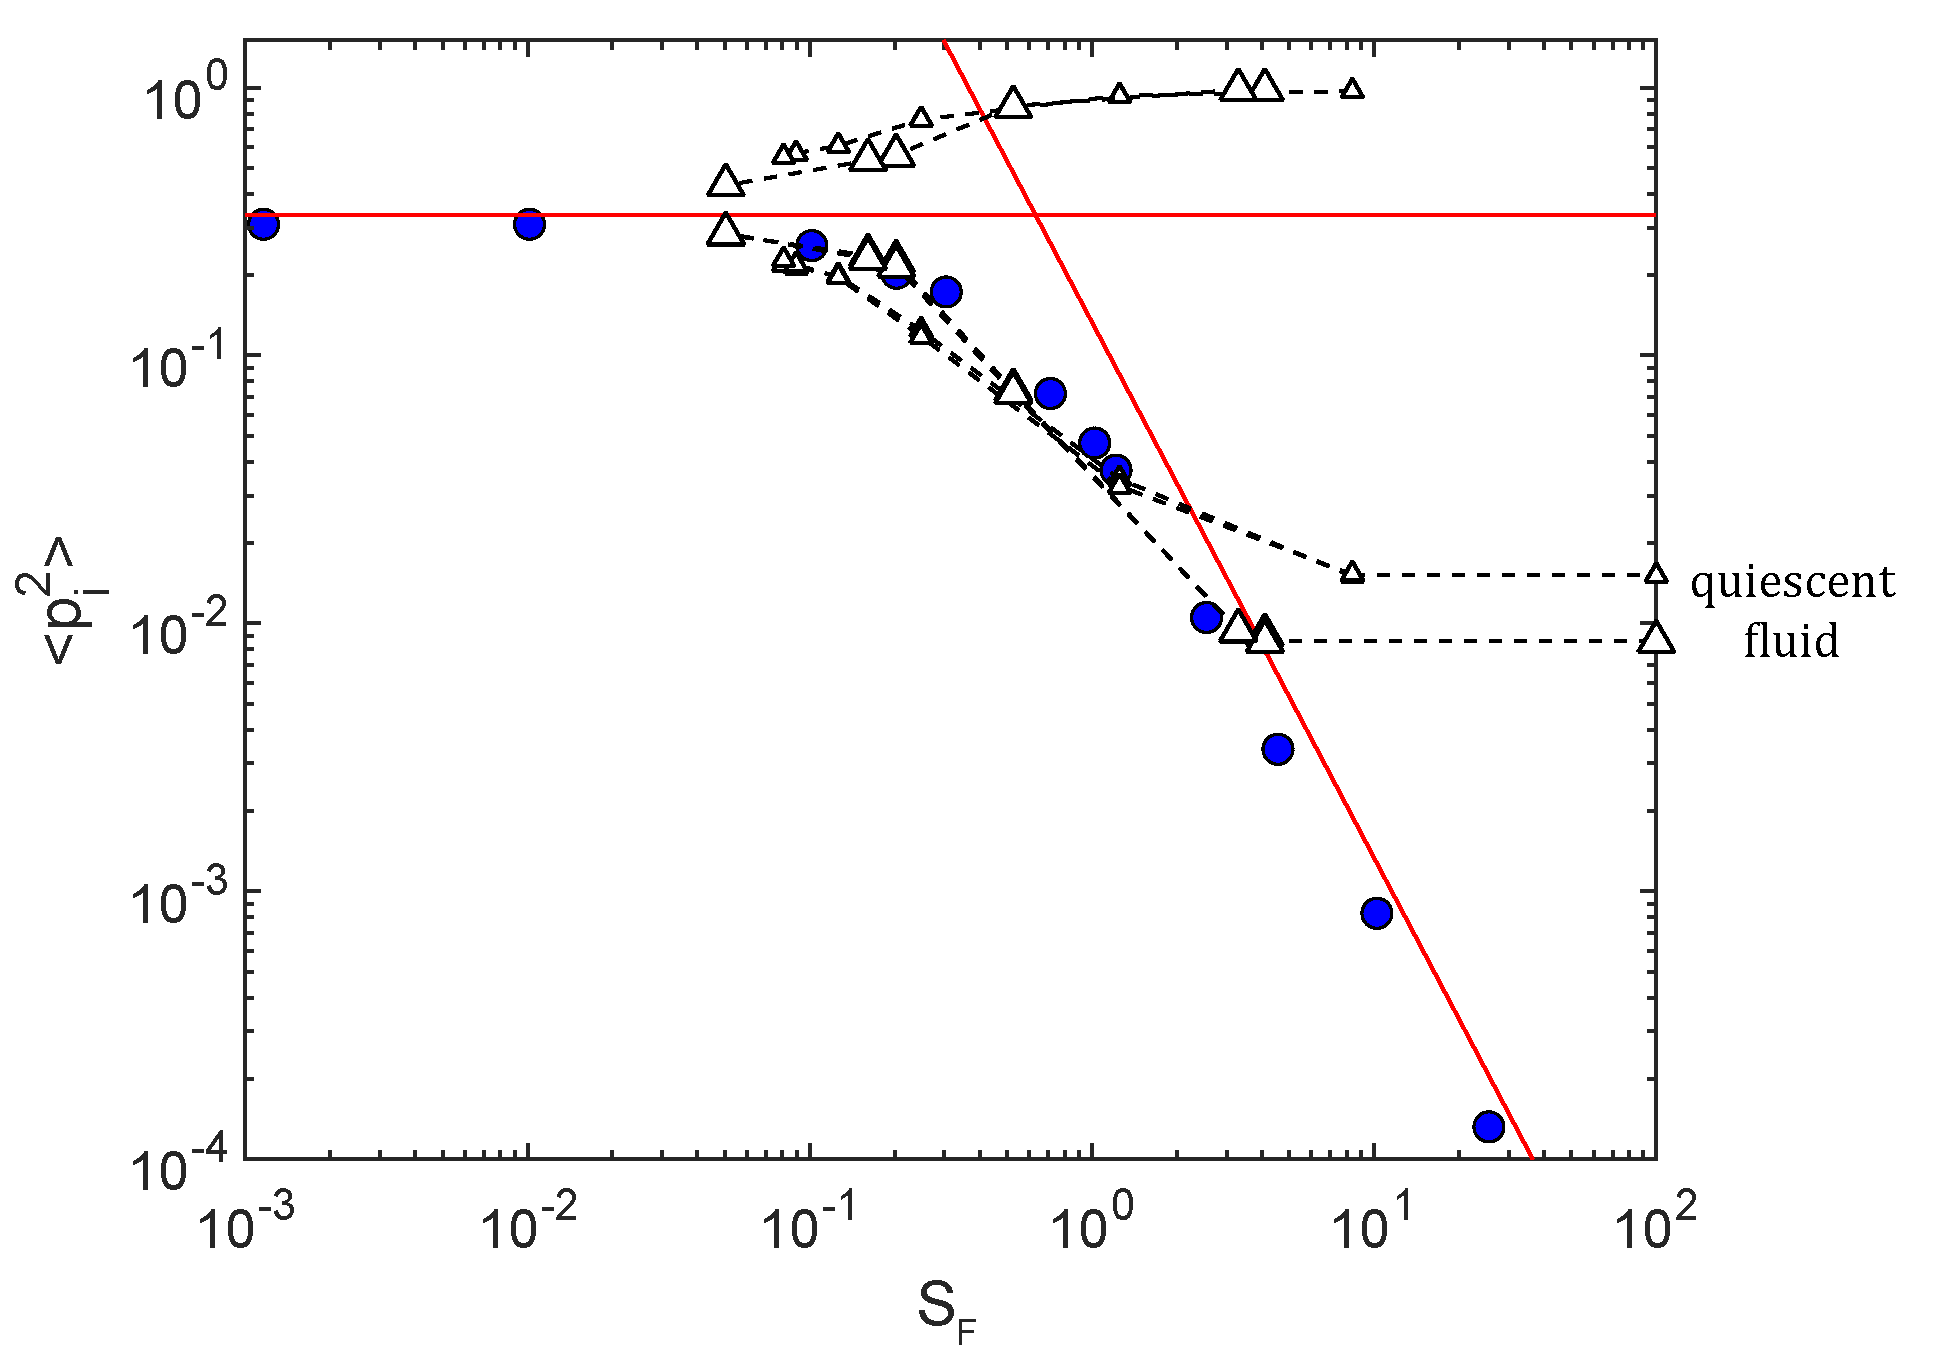
\includegraphics[width=2.7in]{figures/SF_theory.pdf}
\end{minipage}%
\begin{minipage}{.5\textwidth}
  \centering
  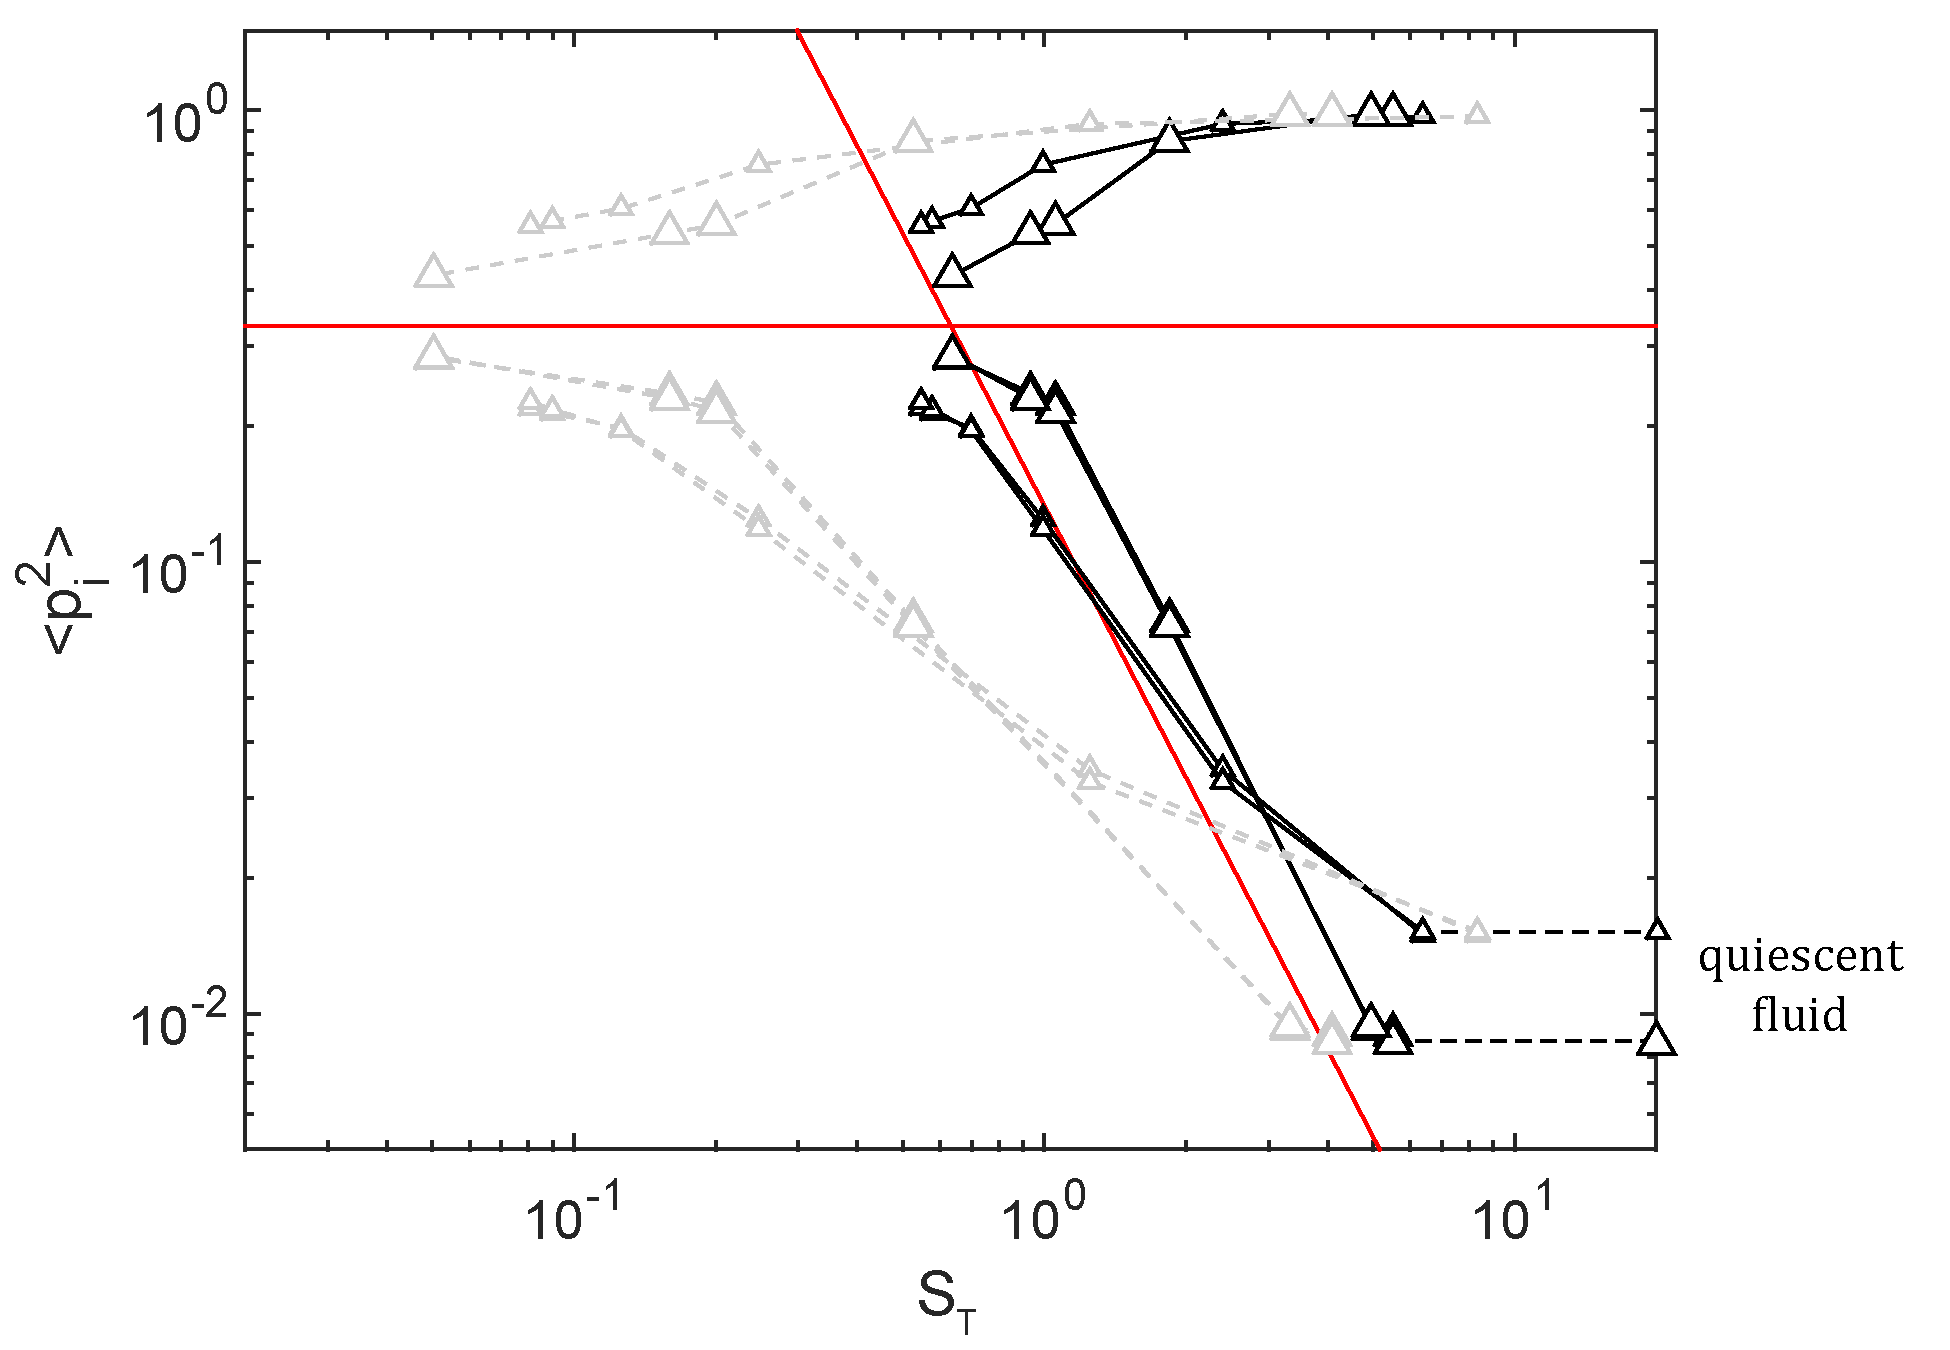
\includegraphics[width=2.7in]{figures/SF_experiments.pdf}
\end{minipage}
  \caption{Mean square of the components of $\mathbf{p}$ as function of settling number. Left: Simulation of fibers at $\textit{Re}_{\lambda}{=}38$ and $S_F{=}\frac{5}{8\log{2\kappa}}(\frac{w}{u_{\eta}})^2$ (for fibers only the z-component, blue circles) and experimental results for small and large triads with $S_T{=}\frac{5}{8\log{2\kappa}}(\frac{w}{u_{l}})^2$ where $u_l{=}\sqrt{15/4}~u_l^T$ (dashed lines, small and large symbols).  Red lines indicate random orientations ($\langle p_z^2\rangle=1/3$) and the strongly aligned limit for fibers where $\langle p_z^2\rangle=\frac{2}{15}S_F^{-2}$.  For triads, the z-component approaches 1, the x- and y-component go to zero in the strongly aligned limit.  Right: Experimental results for small and large triads.  $S_F{=}\frac{\tau_l}{\tau_{\textit{inert}}}$ (black, solid line), where $\tau_l{=}l/u_l$ and $\tau_{\textit{inert}}$ was measured in separate experiments as the return time of a triad to its equilibrium orientation in quiescent fluid. The light gray, dashed lines and triangles show $S_T$ from the left for comparison.}
\label{Fig:mean-square}
\end{figure}

\begin{table}
  \begin{center}
	\def~{\hphantom{0}}
  \begin{tabular}{cccccc} 
	Small particles \\
	\hline
      Turb. Int. & $S_F$  & $w_z$ & $u_l^T (u_l^L)$ & $\tau_l$ &  $\langle p_{i}^2 \rangle$ \\[3pt]
      0.08 & 6.36 (49.34) & -22.58 & 1.66 (0.97) & 2.80 & 0.0150    0.0152    0.9698\\
      0.23 & 2.39 (7.37) & -23.23 & 4.42 (2.46) & 1.05 & 0.0347    0.0326    0.9327\\
      0.38 & 0.99 (1.46) & -24.89 & 10.64 (6.11) & 0.44 & 0.1244    0.1182    0.7574\\
      0.62 & 0.70 (0.74) & -25.28 & 15.14 (8.85) & 0.31 & 0.1982    0.1958    0.6060\\
      0.91 & 0.58 (0.53) & -25.79 & 18.27 (10.85) & 0.25 & 0.2132    0.2177    0.5691 \\
			1.06 & 0.55 (0.48) & -25.71 & 19.25 (11.42) & 0.24 & 0.2195    0.2261    0.5544 \\
			\hline
	Large particles \\
	\hline
      Turb. Int. & $S_F$  & $W_z$ & $u_l^T (u_l^L)$ & $\tau_l$ & $\langle p_{i}^2 \rangle$ \\[3pt]
       0.07 & 5.49 (24.08) & -35.73 & 3.76 (2.29) & 2.47 &  0.0090    0.0086    0.9823\\
       0.10 & 4.95 (19.61) & -35.76 & 4.17 (2.45) & 2.23 &  0.0093    0.0094    0.9814\\
       0.29 & 1.84 (3.10) & -38.30 & 11.23 (6.74) & 0.83 & 0.0743    0.0724    0.8533\\
       0.28 & 1.05 (1.19) & -41.36 & 19.59 (12.09) & 0.47 & 0.2251    0.2163    0.5586\\
       0.37 & 0.94 (0.95) & -41.48 & 22.03 (13.53) & 0.42 & 0.2358    0.2301    0.5341\\
			 0.95 & 0.64 (0.30) & -34.01 & 32.29 (19.97) & 0.29 & 0.2834    0.2859    0.4307\\
  \end{tabular}
  \caption{settling number for triads defined empirically $S_F{=}\frac{\tau_l}{\tau_{\textit{inert}}}$ (and analogue to fibers $S_F{=}(\frac{w}{u_l})^2$) where $\tau_{\textit{inert}}{=}0.44$ s for small triads and $\tau_{\textit{inert}}{=}0.45$ s for large triads.  $w{=}\langle u_p \rangle {-} \langle u_f \rangle$ local relative velocity measured using tracers within a sphere of radius $6l$ around the triads; $u_p$ and $u_f$ particle and local fluid velocity; $W{=}\langle u_p \rangle{-}\langle U_f \rangle$ mean relative velocity; $u_l^T (u_l^L)$, magnitude of transverse (longitudinal) rms velocity-difference at scale $l$; $\langle p_{i}^2 \rangle$, components of the mean square particle orientation.}
  \label{tab:kd2}
  \end{center}
\end{table}

\section{Sedimentation Statistics}
In this section, we present the sedimentation statistics of fibers and triads in quiescent fluid to establish a reference system. The results of the experiments with triads under varying levels of turbulence are presented later.  A simple model based on slender body theory is compared to the results.  Details of the model and the variables/coordinate system are described in the Appendix.

TURBULENCE-- The following Figures~\ref{Fig:wz}, \ref{Fig:wz-norm} and \ref{Fig:wz-sigma} show the mean sedimentation rate in the direction of gravity $w_z$ and the corresponding standard deviation $\sigma_{w_z}$ of small triads conditioned on their orientation $p_z$ for 6 different turbulence intensities (colormap: from low/blue to large/red).  Figures on the left show the relative sedimentation rate with respect to the local fluid velocity, $\mathbf{w}=(\mathbf{u}_p{-}\mathbf{u}_f)$ and Figures on the right show the relative sedimentation rate with respect to the mean fluid velocity $\mathbf{W}=(\mathbf{u}_p{-}\mathbf{U}_f)$.  The local fluid velocity around triads was measured with small tracer particles within a sphere of radius 6$l$.  Smaller radii yielded qualitatively the same results, however, fewer tracer particles result in much more measurement noise.  Figure~\ref{Fig:wz-norm} shows the sedimentation rate normalized by the sedimentation rate at $p_z=1$ and can be directly compared to the top curves in Fig.~\ref{Fig:particle-velocity}.  The black lines in these Figures accounts for the effective aspect ratio of a disk (dashed lines) and $M_\parallel/M_\perp=1.9$ (dotted lines).  

\begin{figure}
\centering
\begin{minipage}{.5\textwidth}
  \centering
  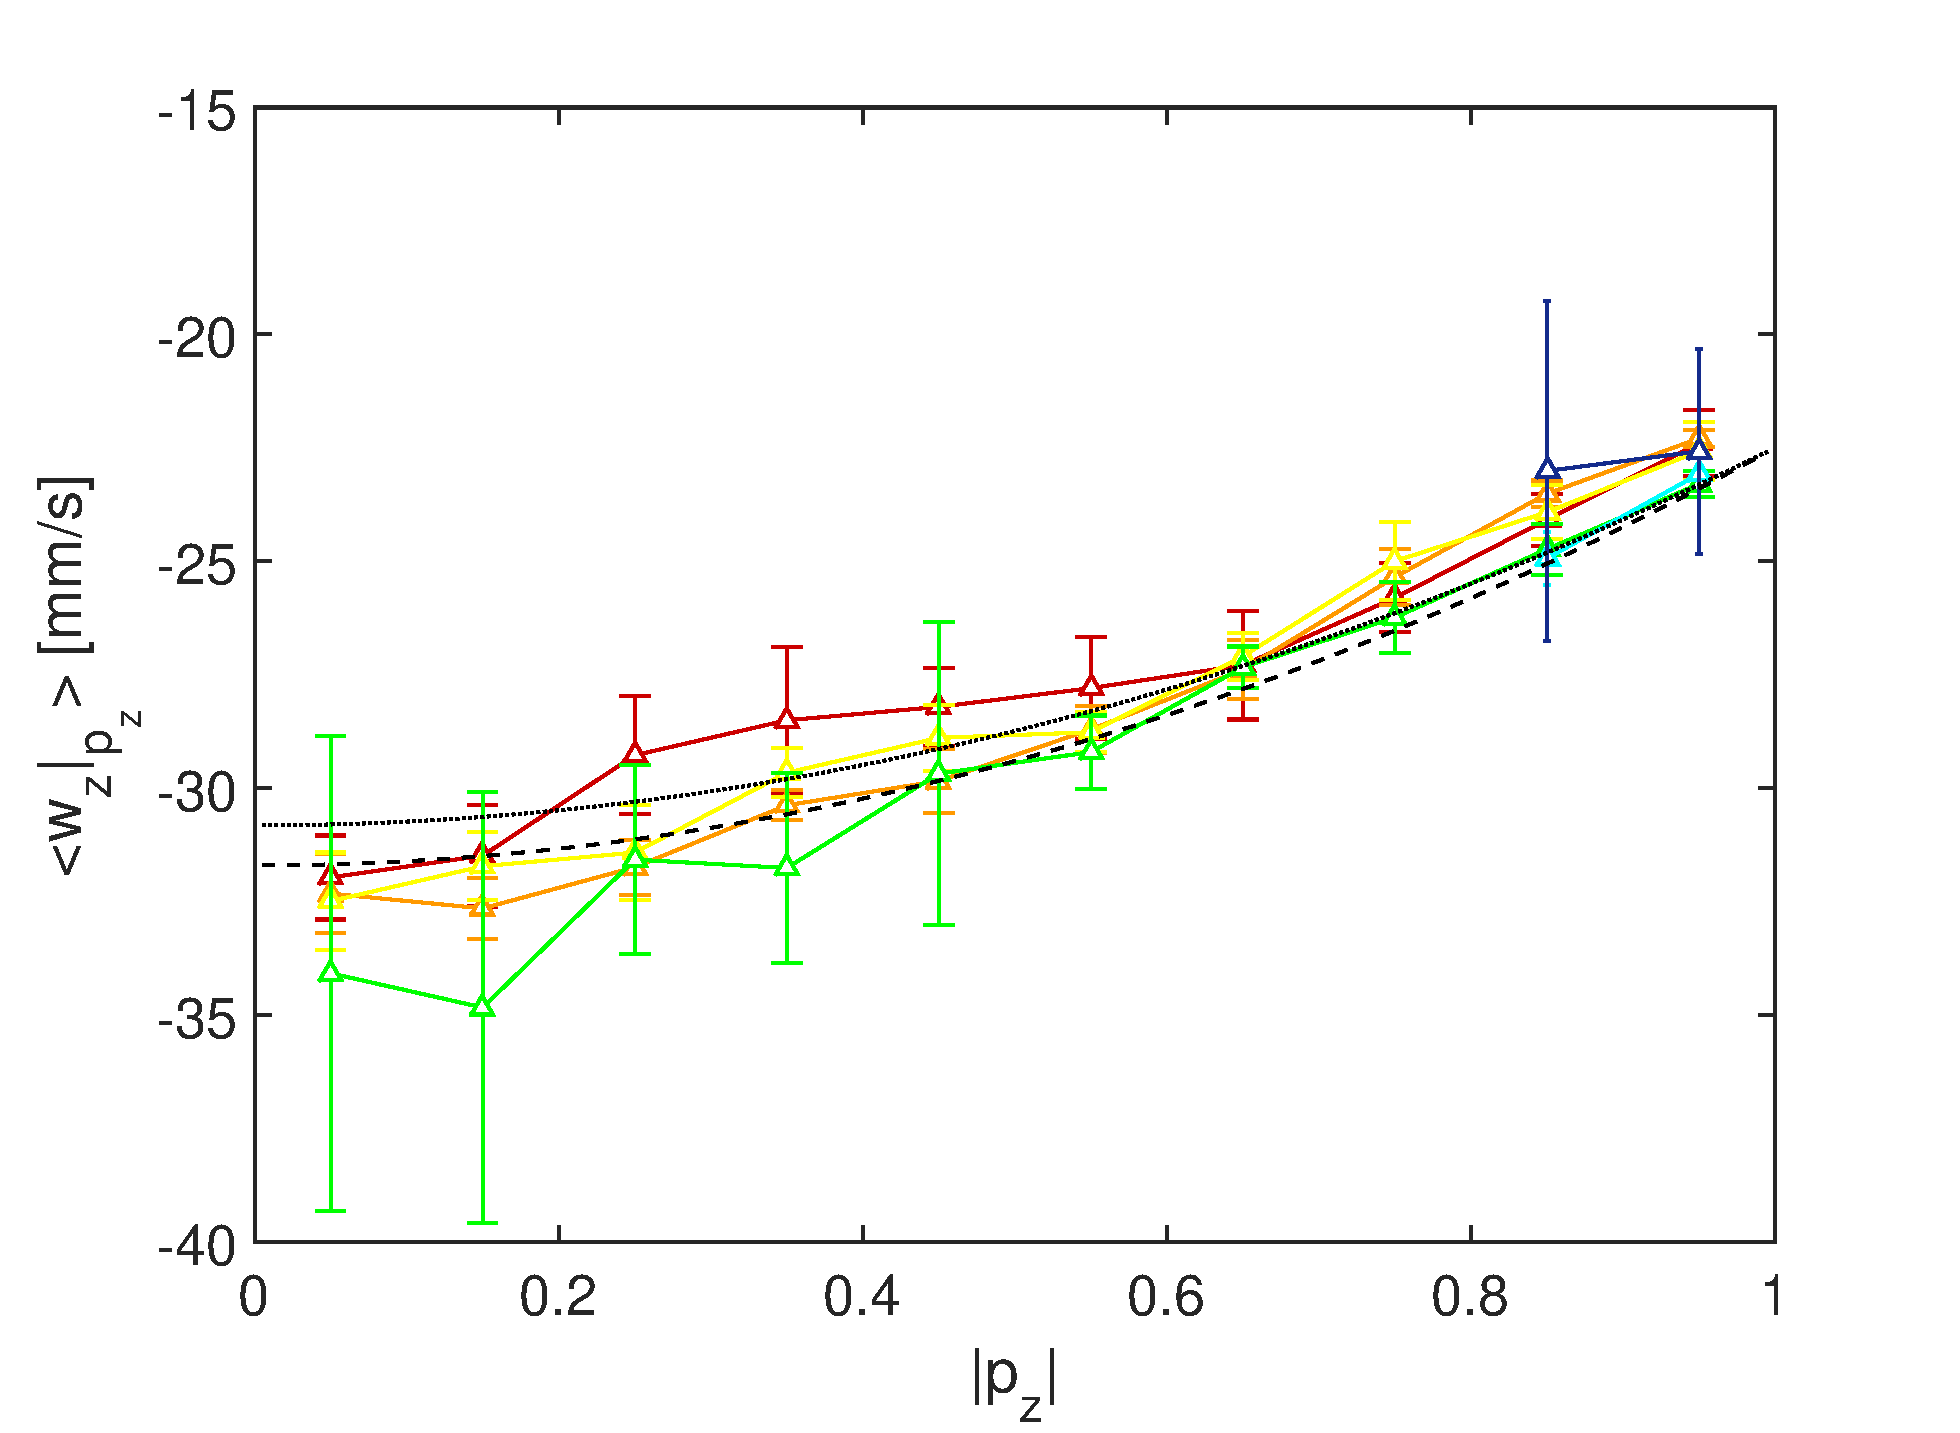
\includegraphics[width=2.9in]{figures/wz-local-small.pdf}
\end{minipage}%
\begin{minipage}{.5\textwidth}
  \centering
  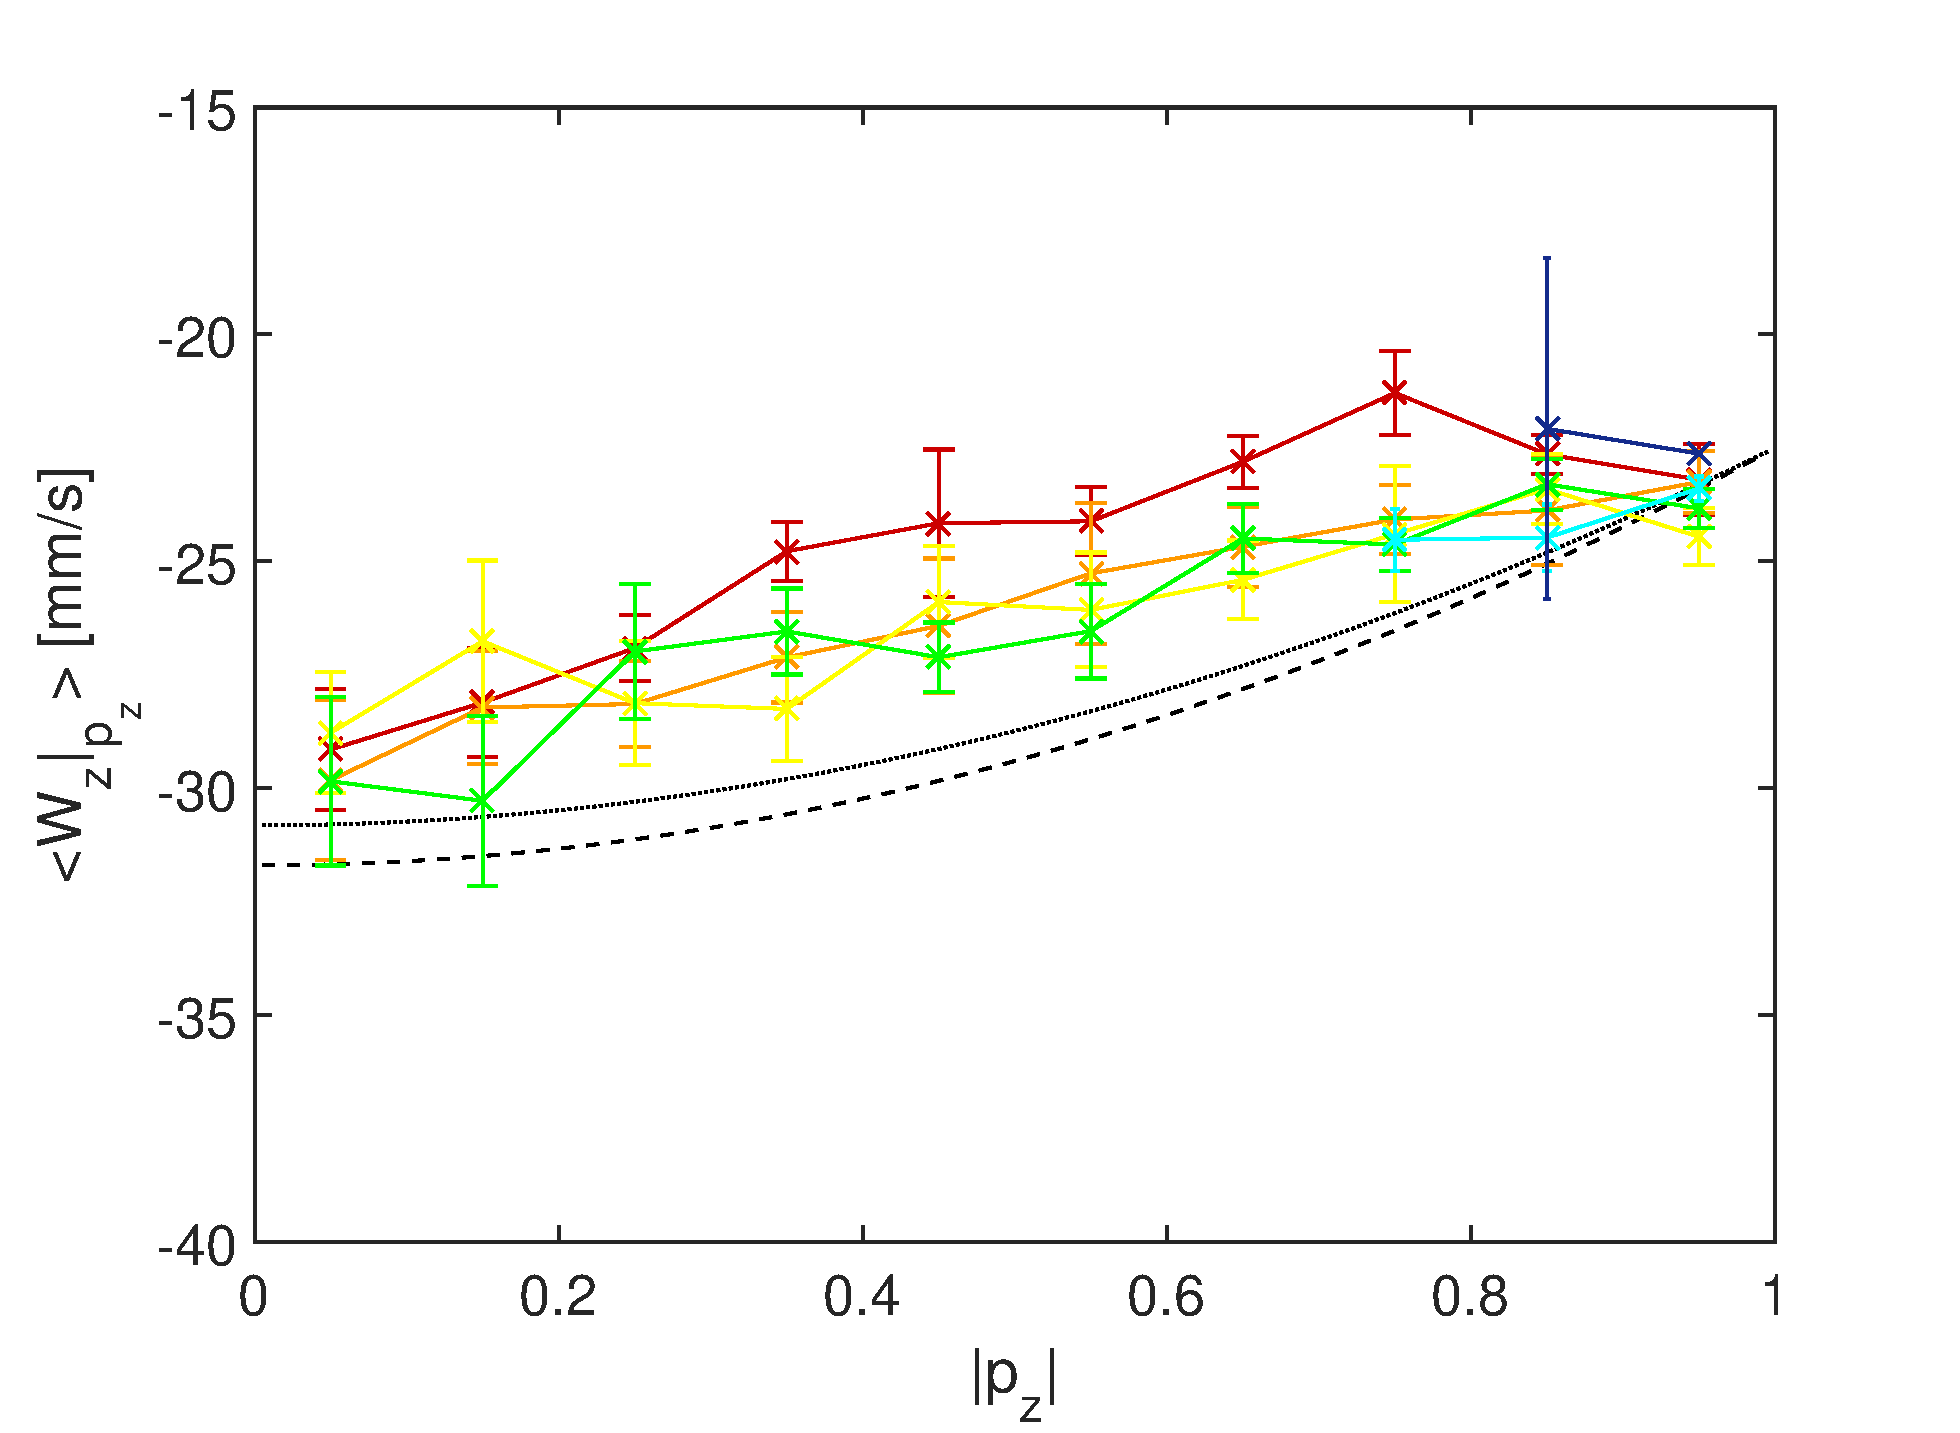
\includegraphics[width=2.9in]{figures/wz-U-small.pdf}
\end{minipage}
\caption{Mean z-component of the relative particle velocity, conditioned on $|p_z|$ for small particles. Left: $\mathbf{w}{=}(\mathbf{u}_p{-}\mathbf{u}_f)$. Right: $\mathbf{W}{=}(\mathbf{u}_p{-}\mathbf{U}_f)$. The prediction using the model from Appendix B are shown as the black dashed line ($M_\parallel/M_\perp{=}2$) and black dotted line ($M_\parallel/M_\perp{=}1.9$)}
\label{Fig:wz}
\end{figure}

\begin{figure}
\centering
\begin{minipage}{.5\textwidth}
  \centering
  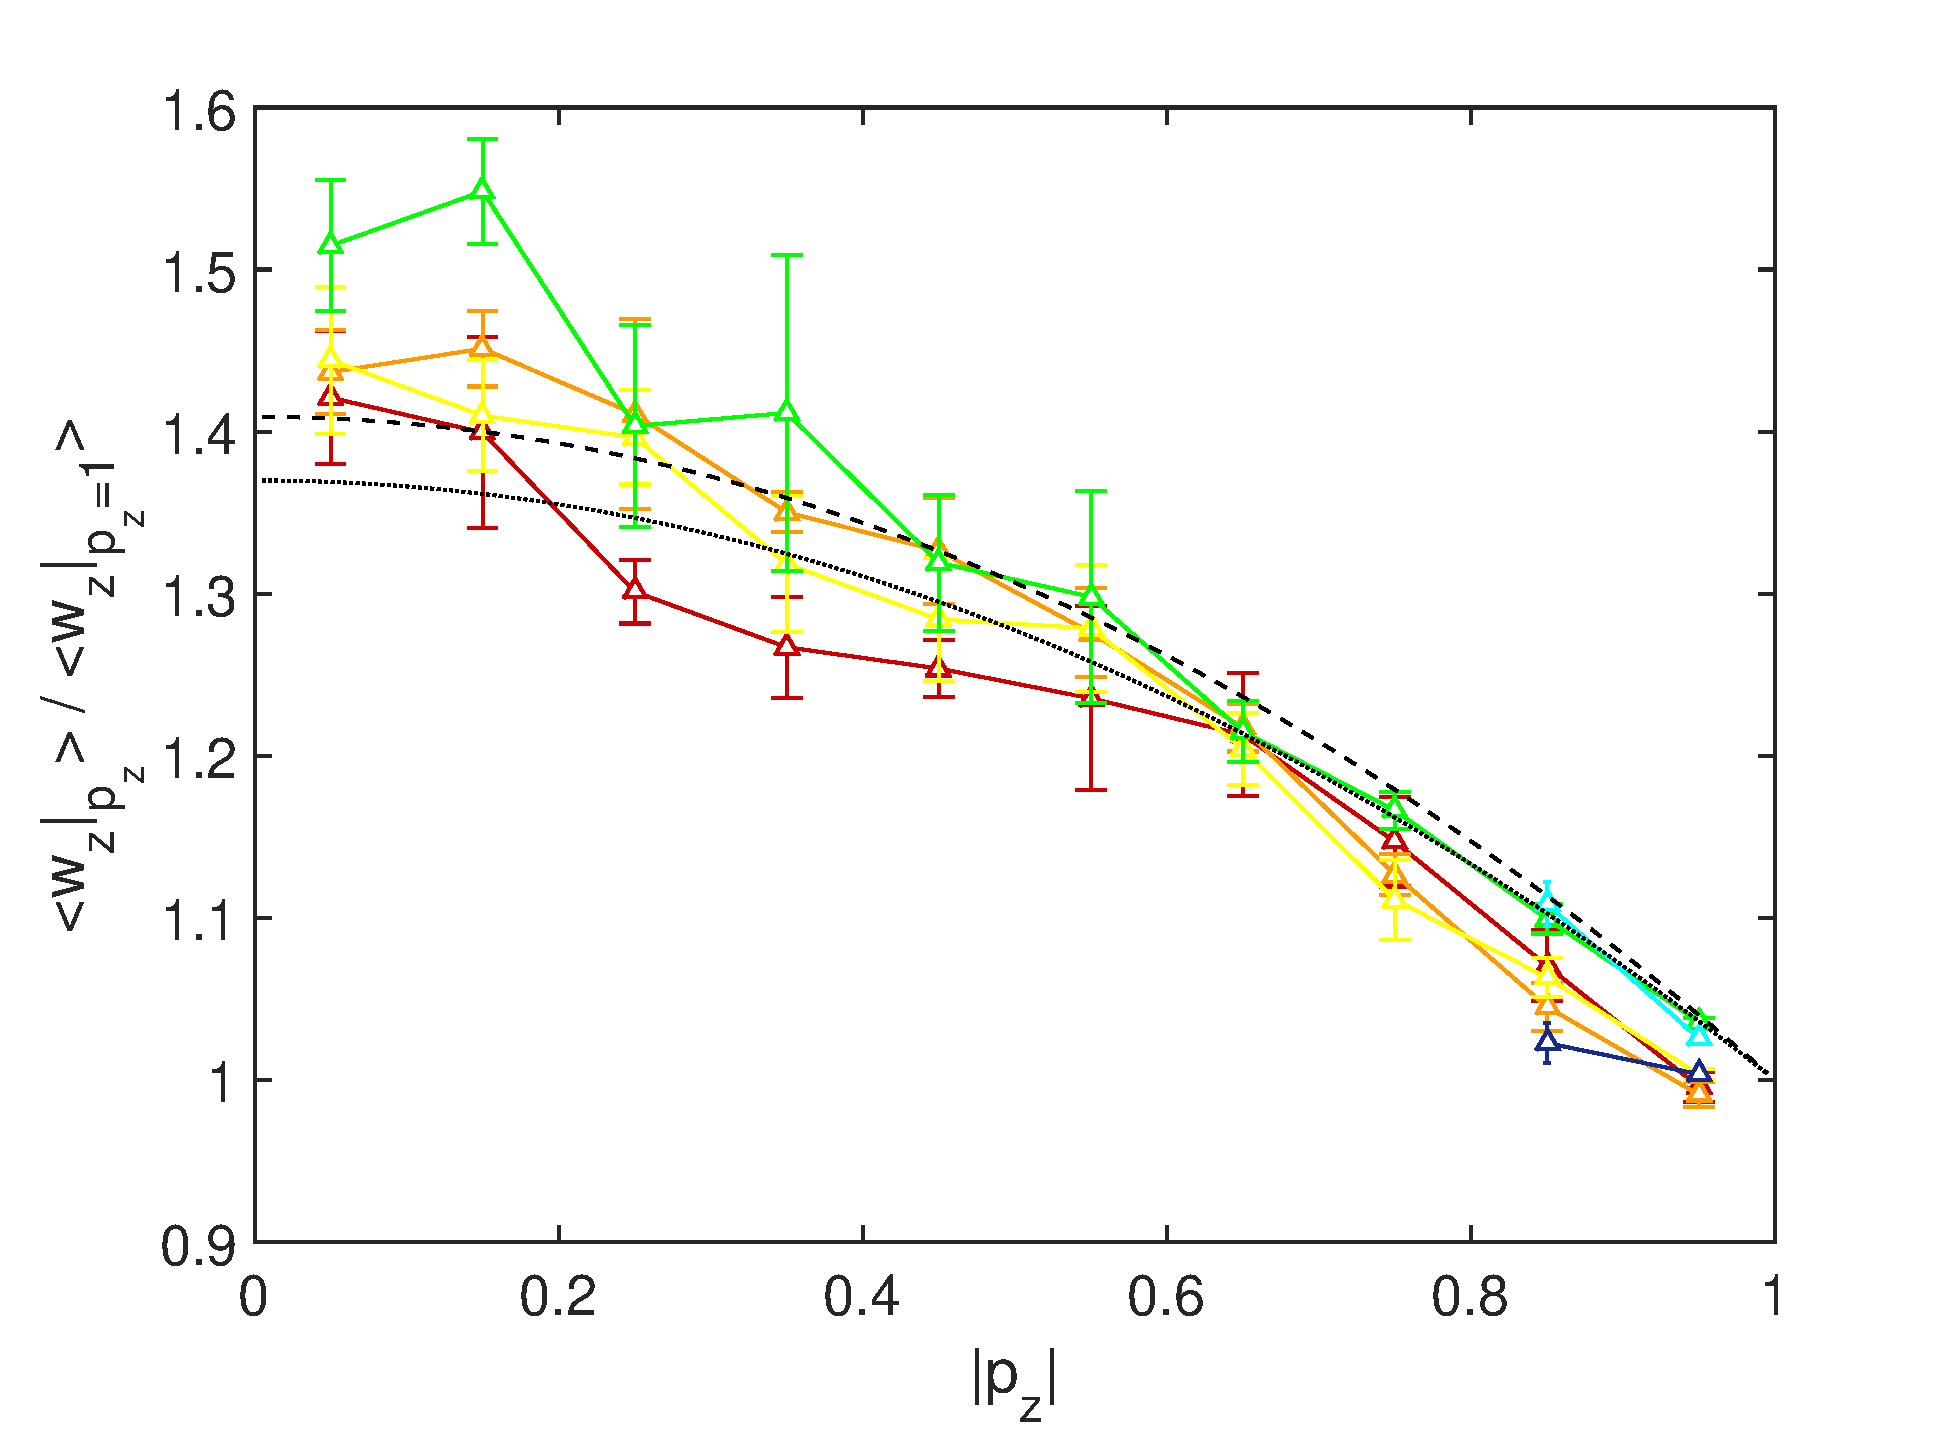
\includegraphics[width=2.9in]{figures/wz-local-norm-small.pdf}
\end{minipage}%
\begin{minipage}{.5\textwidth}
  \centering
  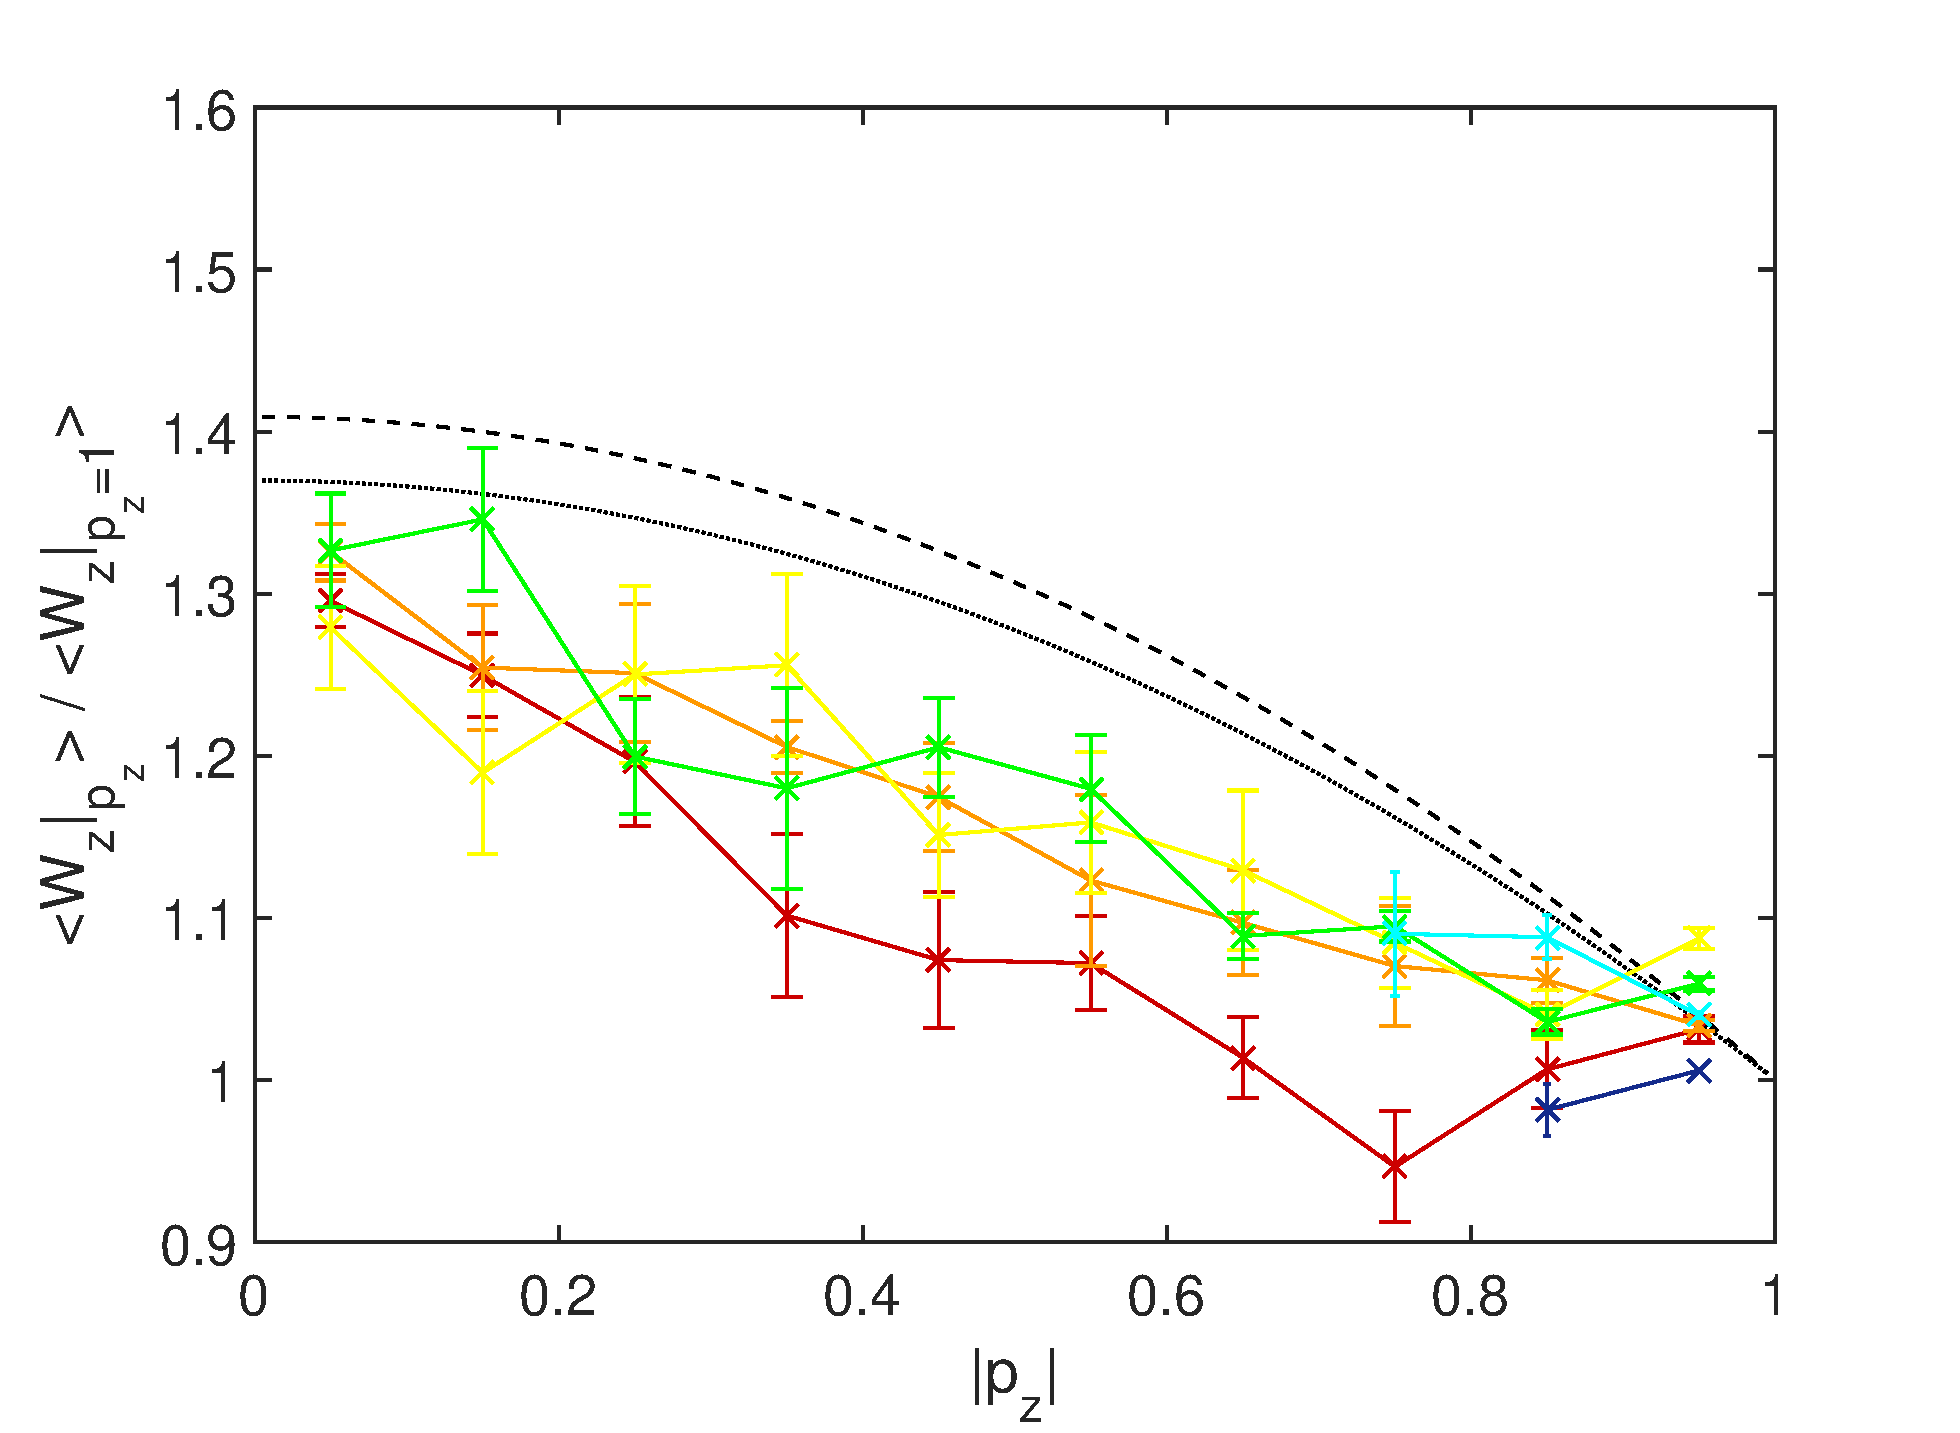
\includegraphics[width=2.9in]{figures/wz-U-norm-small.pdf}
\end{minipage}
\caption{Mean z-component of the relative particle velocity, conditioned on $|p_z|$, normalized by the particle velocity in quiescent fluid (small particles). Left: $\mathbf{w}{=}(\mathbf{u}_p{-}\mathbf{u}_f)$. Right: $\mathbf{W}{=}(\mathbf{u}_p{-}\mathbf{U}_f)$. Symbols are the same as in Fig.~\ref{Fig:wz}. }
\label{Fig:wz-norm}
\end{figure}

\begin{figure}
\centering
\begin{minipage}{.5\textwidth}
  \centering
  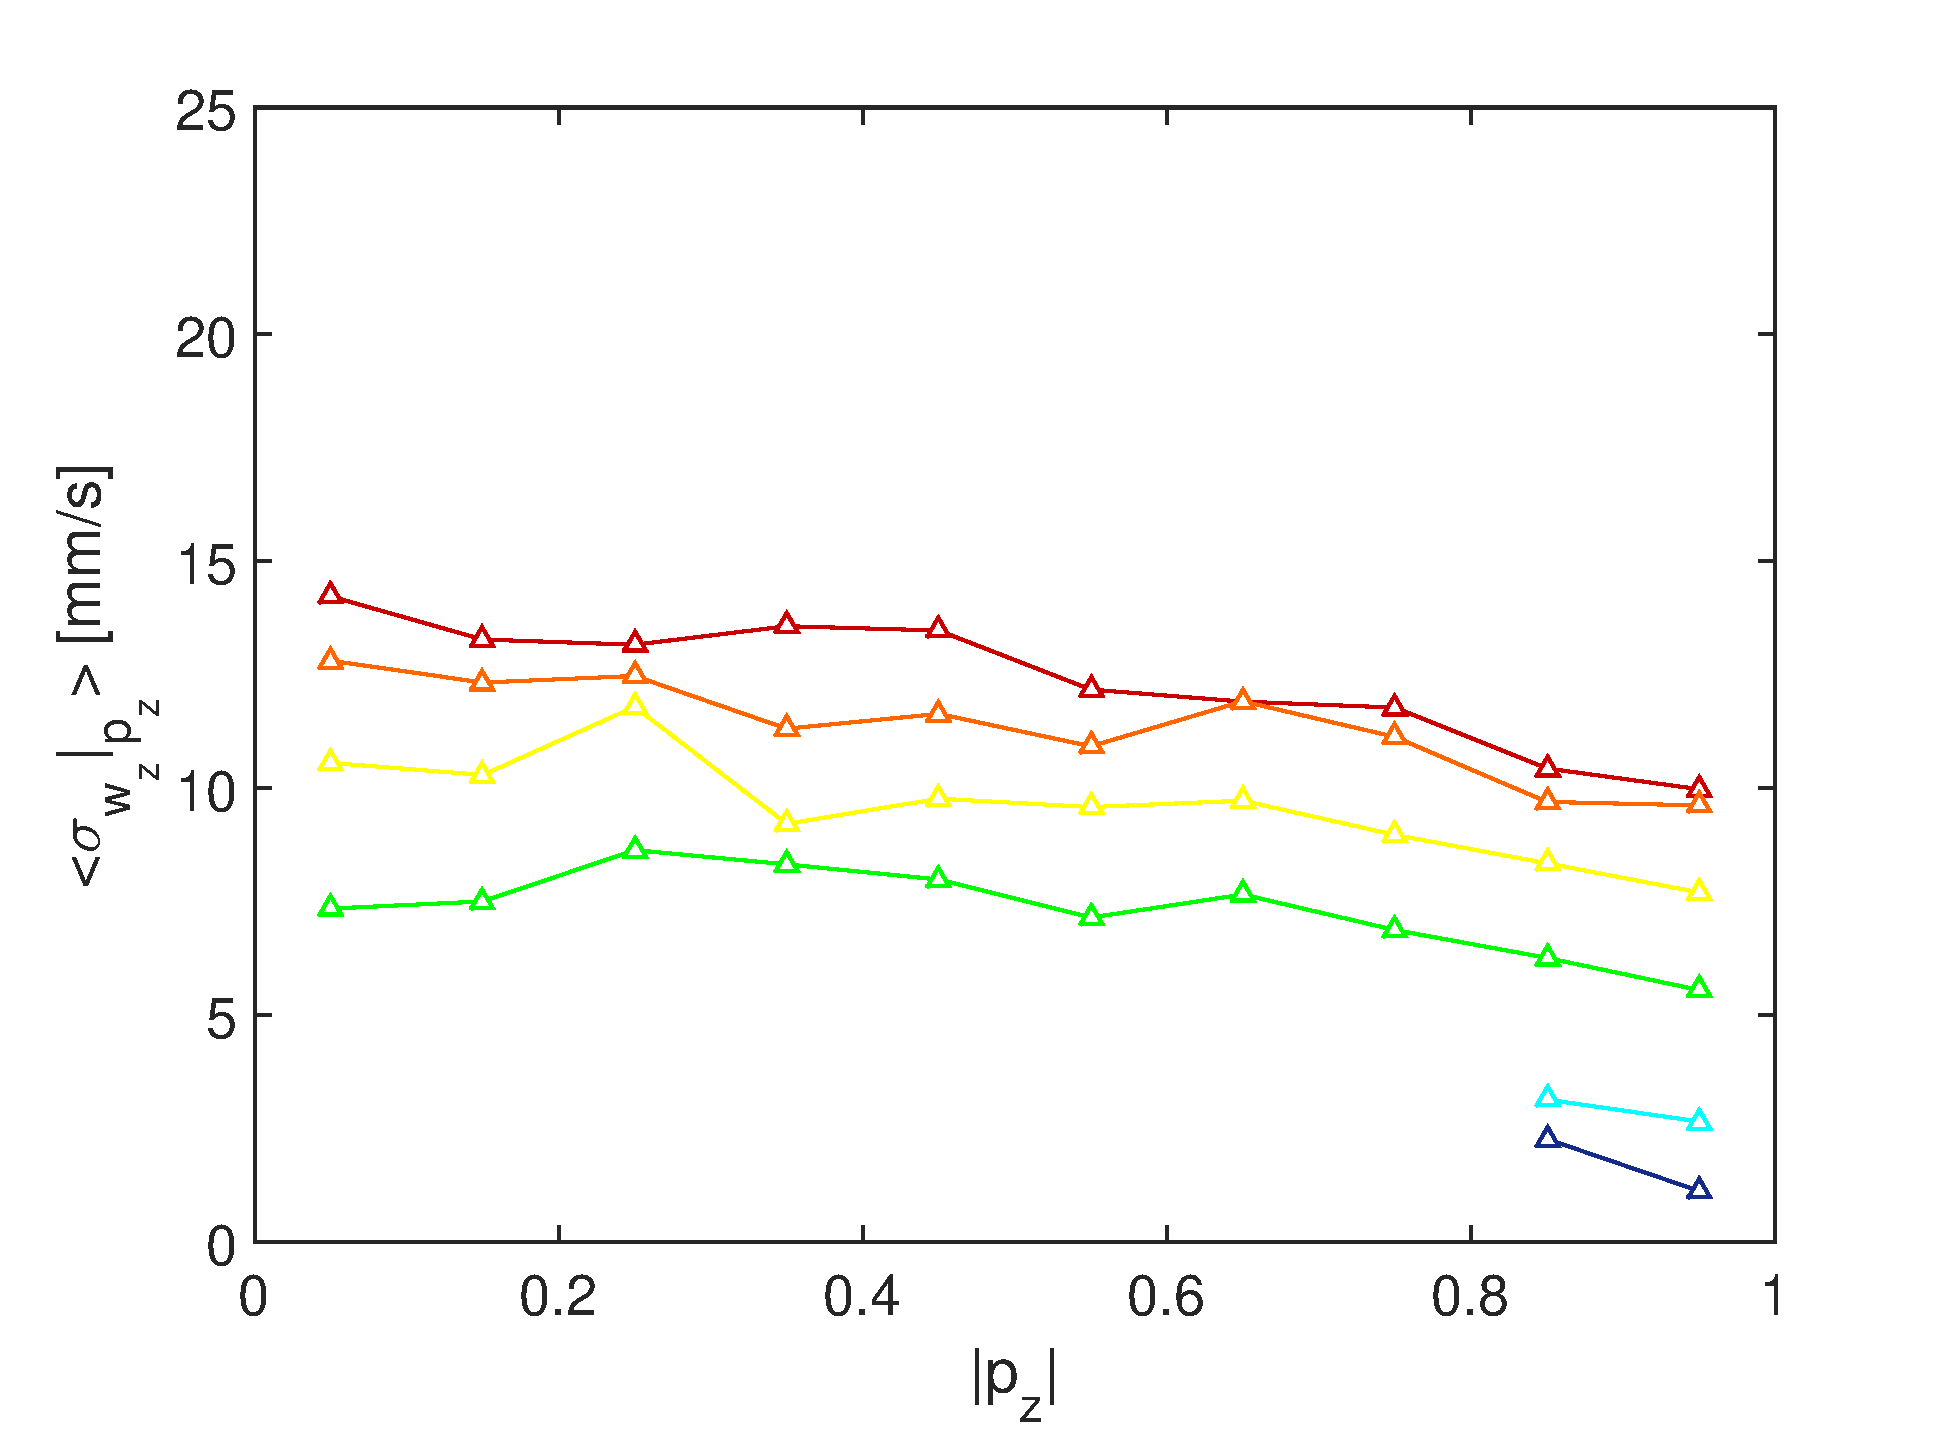
\includegraphics[width=2.9in]{figures/wz-local-sigma-small.pdf}
\end{minipage}%
\begin{minipage}{.5\textwidth}
  \centering
  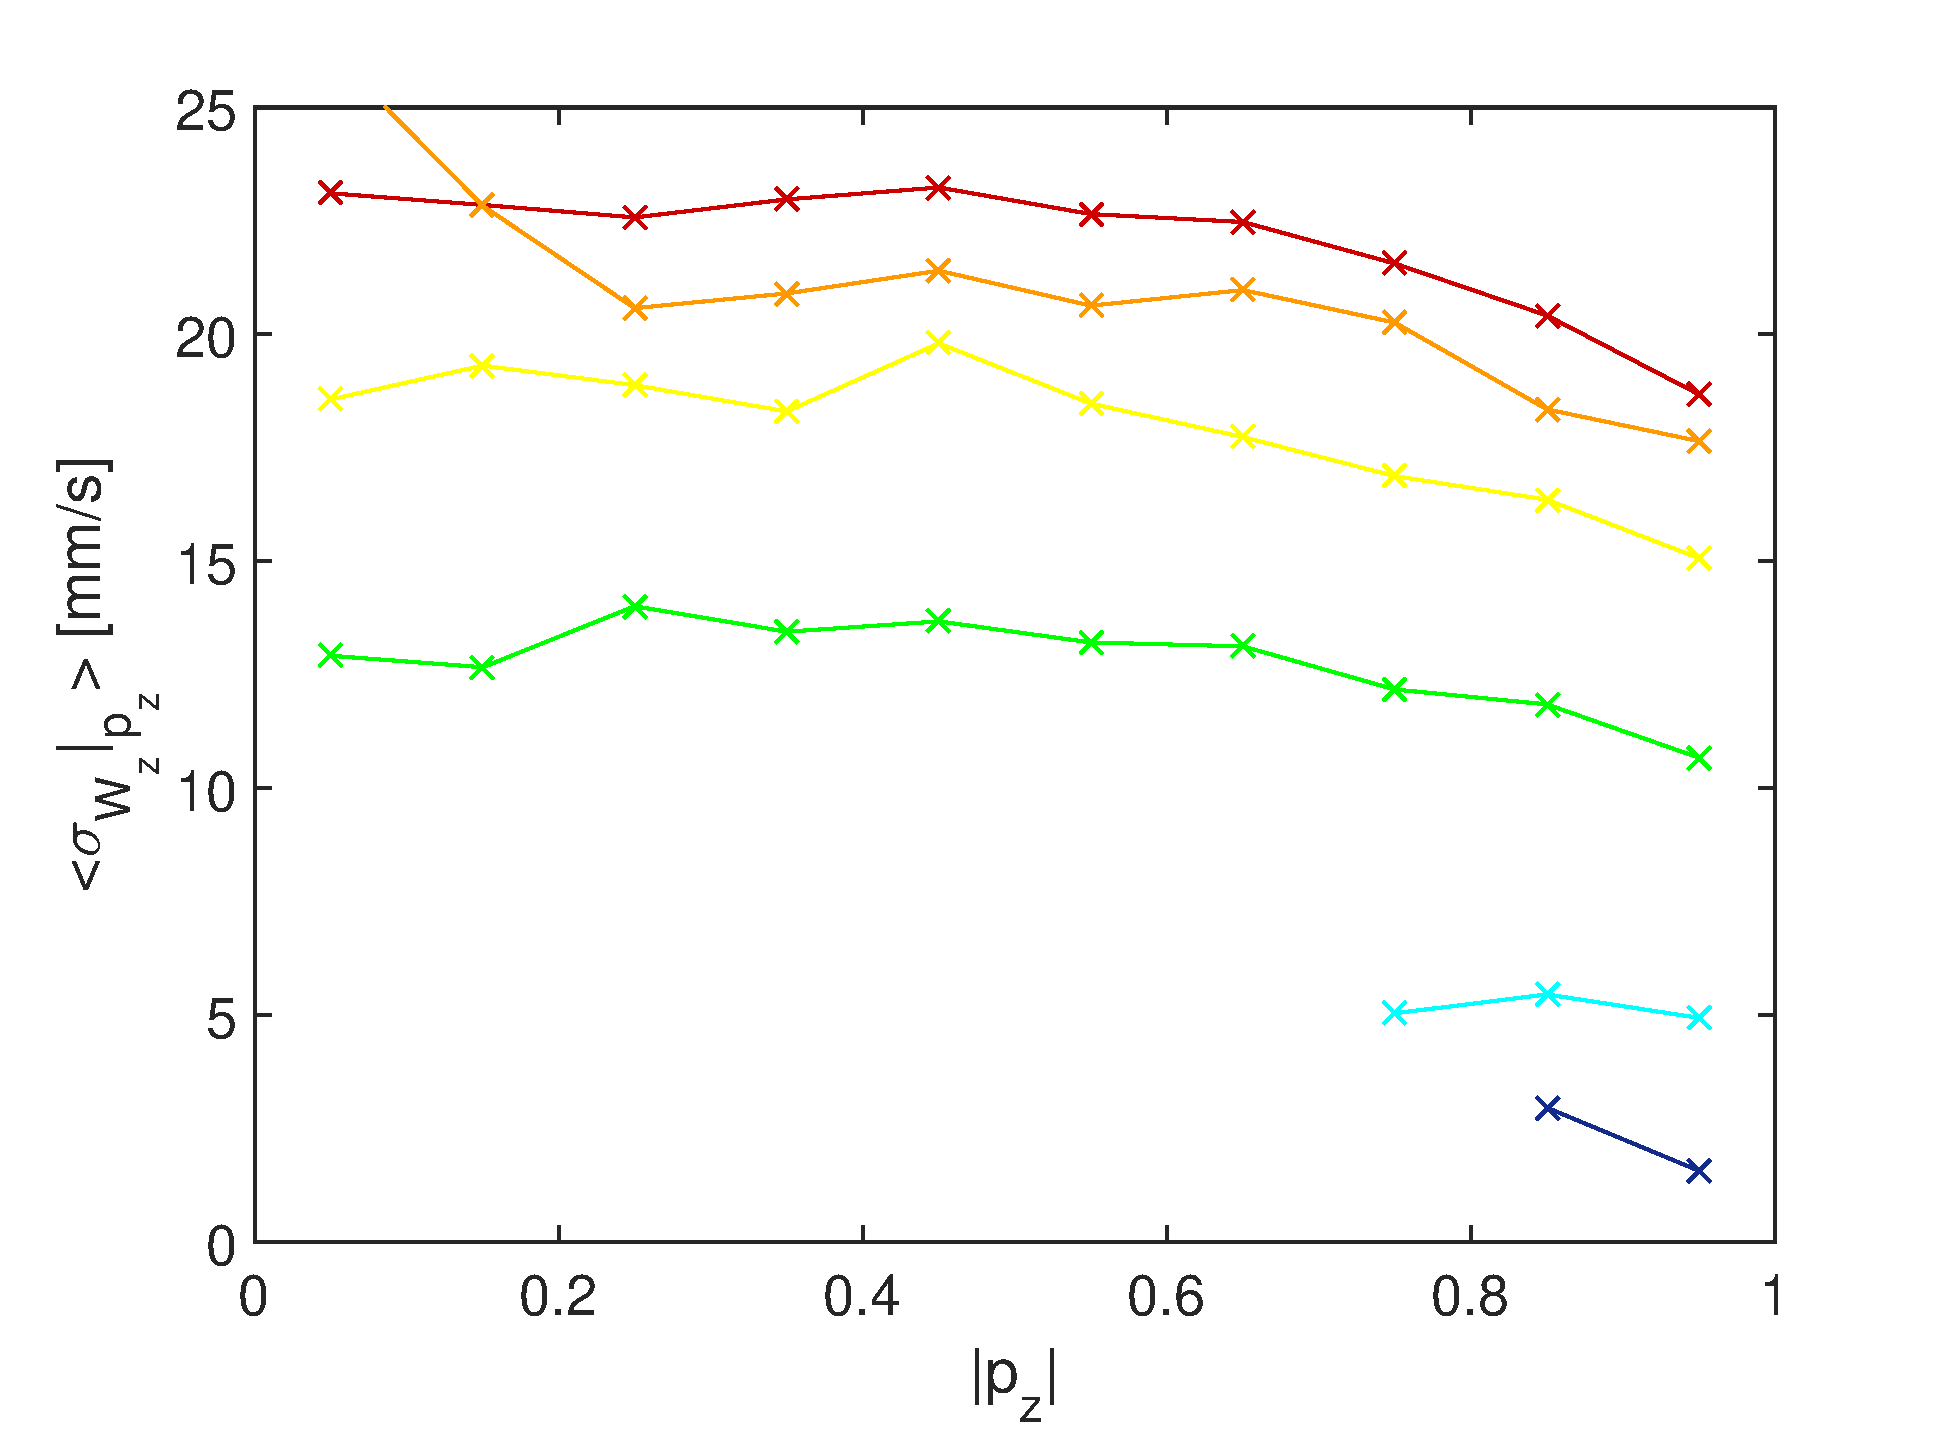
\includegraphics[width=2.9in]{figures/wz-U-sigma-small.pdf}
\end{minipage}
\caption{Standard deviation of the z-component of the relative particle velocity, conditioned on $|p_z|$, for small particles. Left: $\sigma_z=(\langle w_z^2 \rangle-\langle w_z \rangle^2)^{\frac{1}{2}}$. Right: $\sigma_z=(\langle W_z^2 \rangle-\langle W_z \rangle^2)^{\frac{1}{2}}$.}
\label{Fig:wz-sigma}
\end{figure}

Figure~\ref{Fig:alpha}

\begin{figure}
\centering
\begin{minipage}{.5\textwidth}
  \centering
  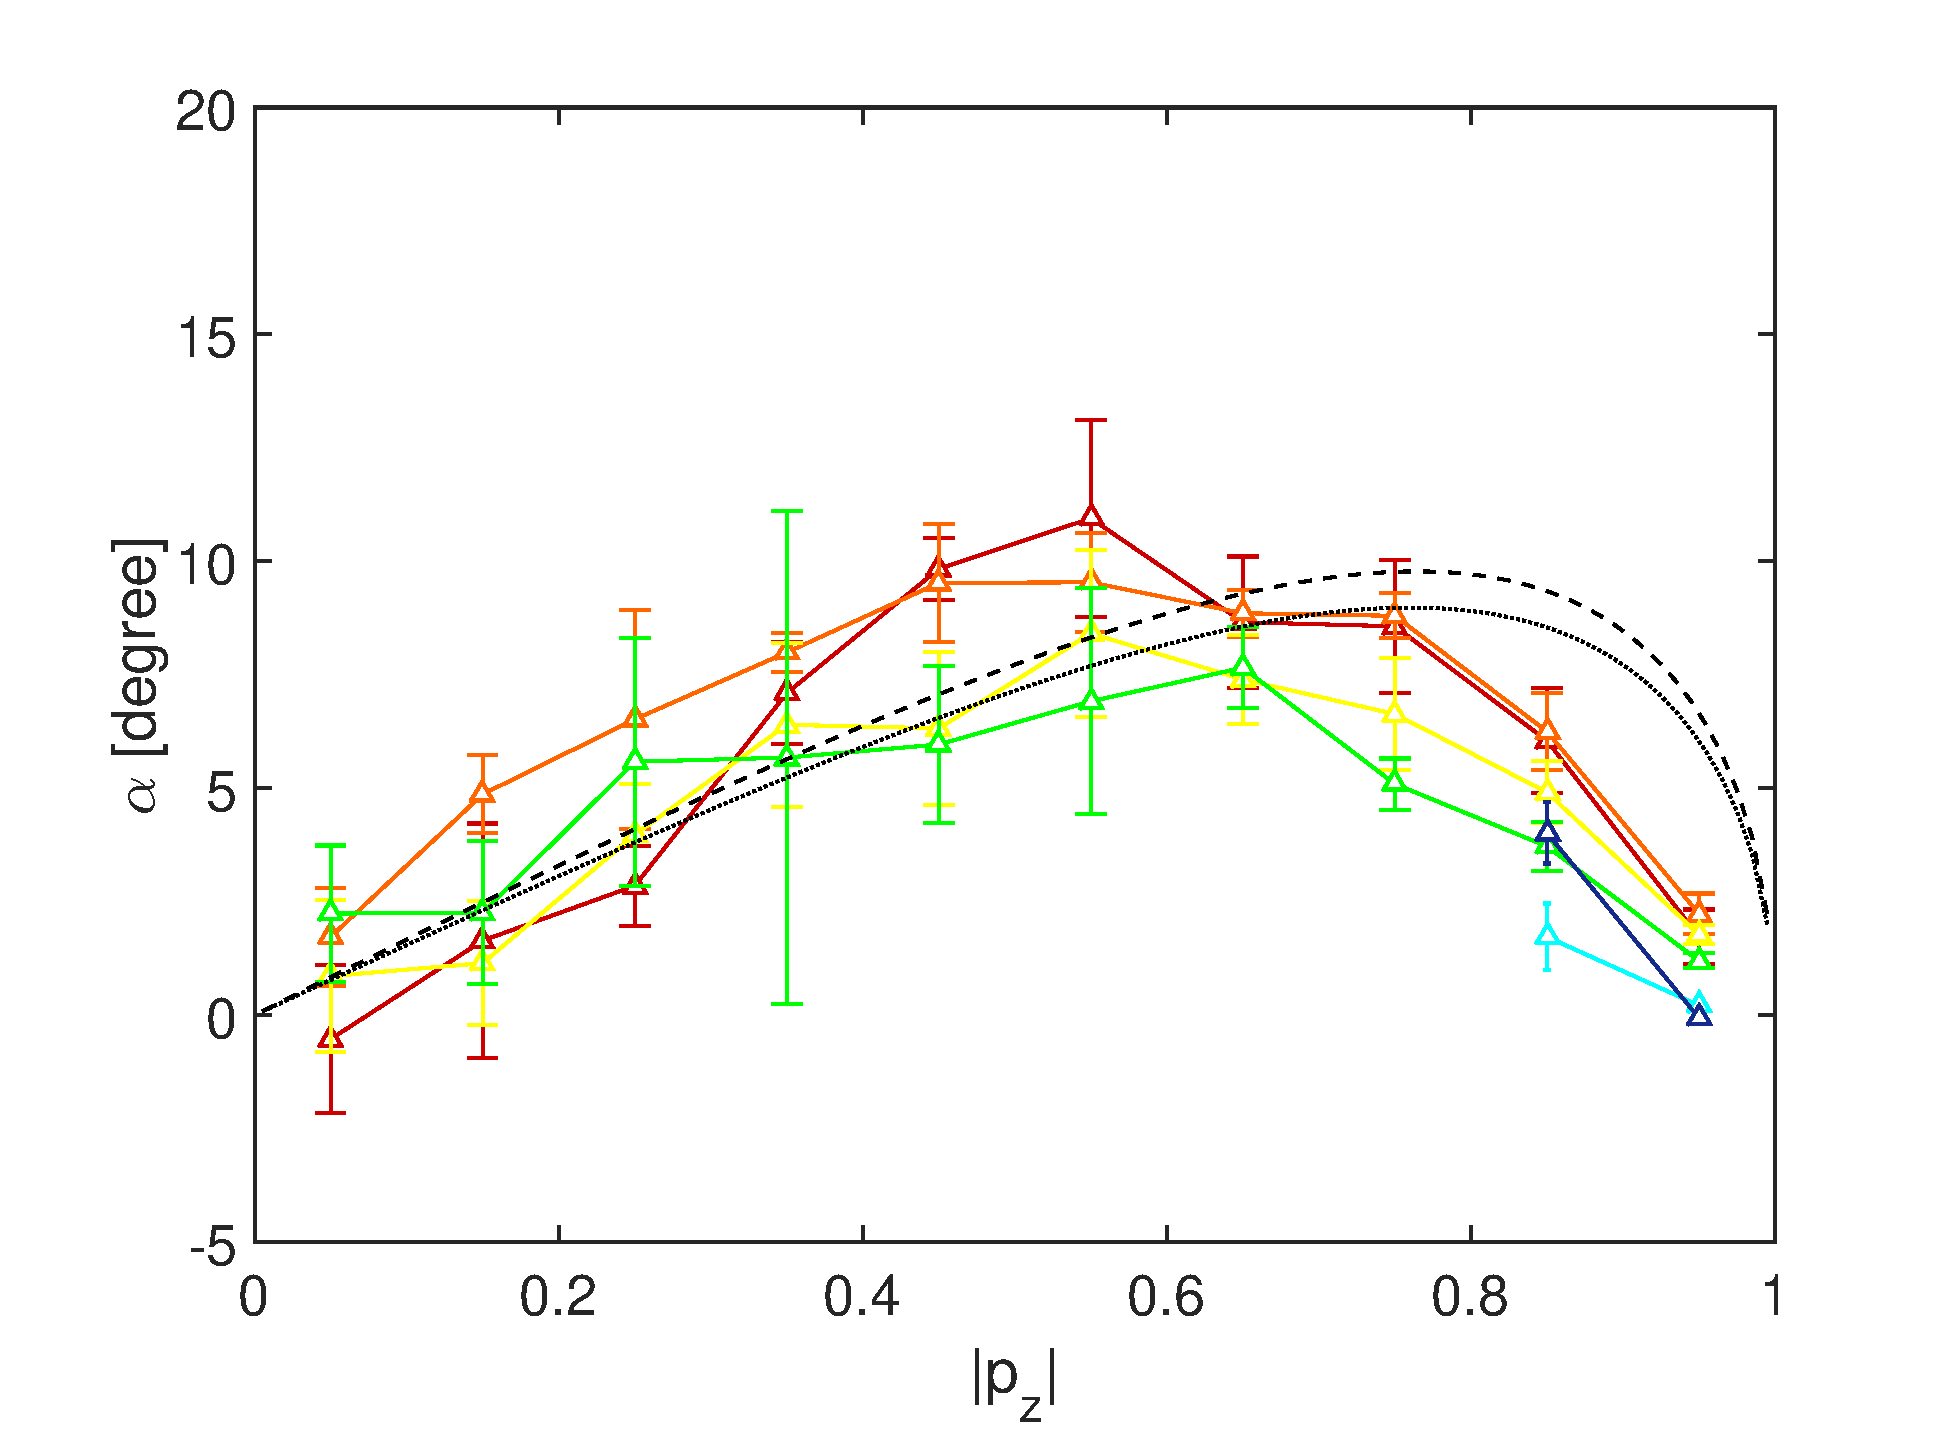
\includegraphics[width=2.9in]{figures/alpha-local-small.pdf}
\end{minipage}%
\begin{minipage}{.5\textwidth}
  \centering
  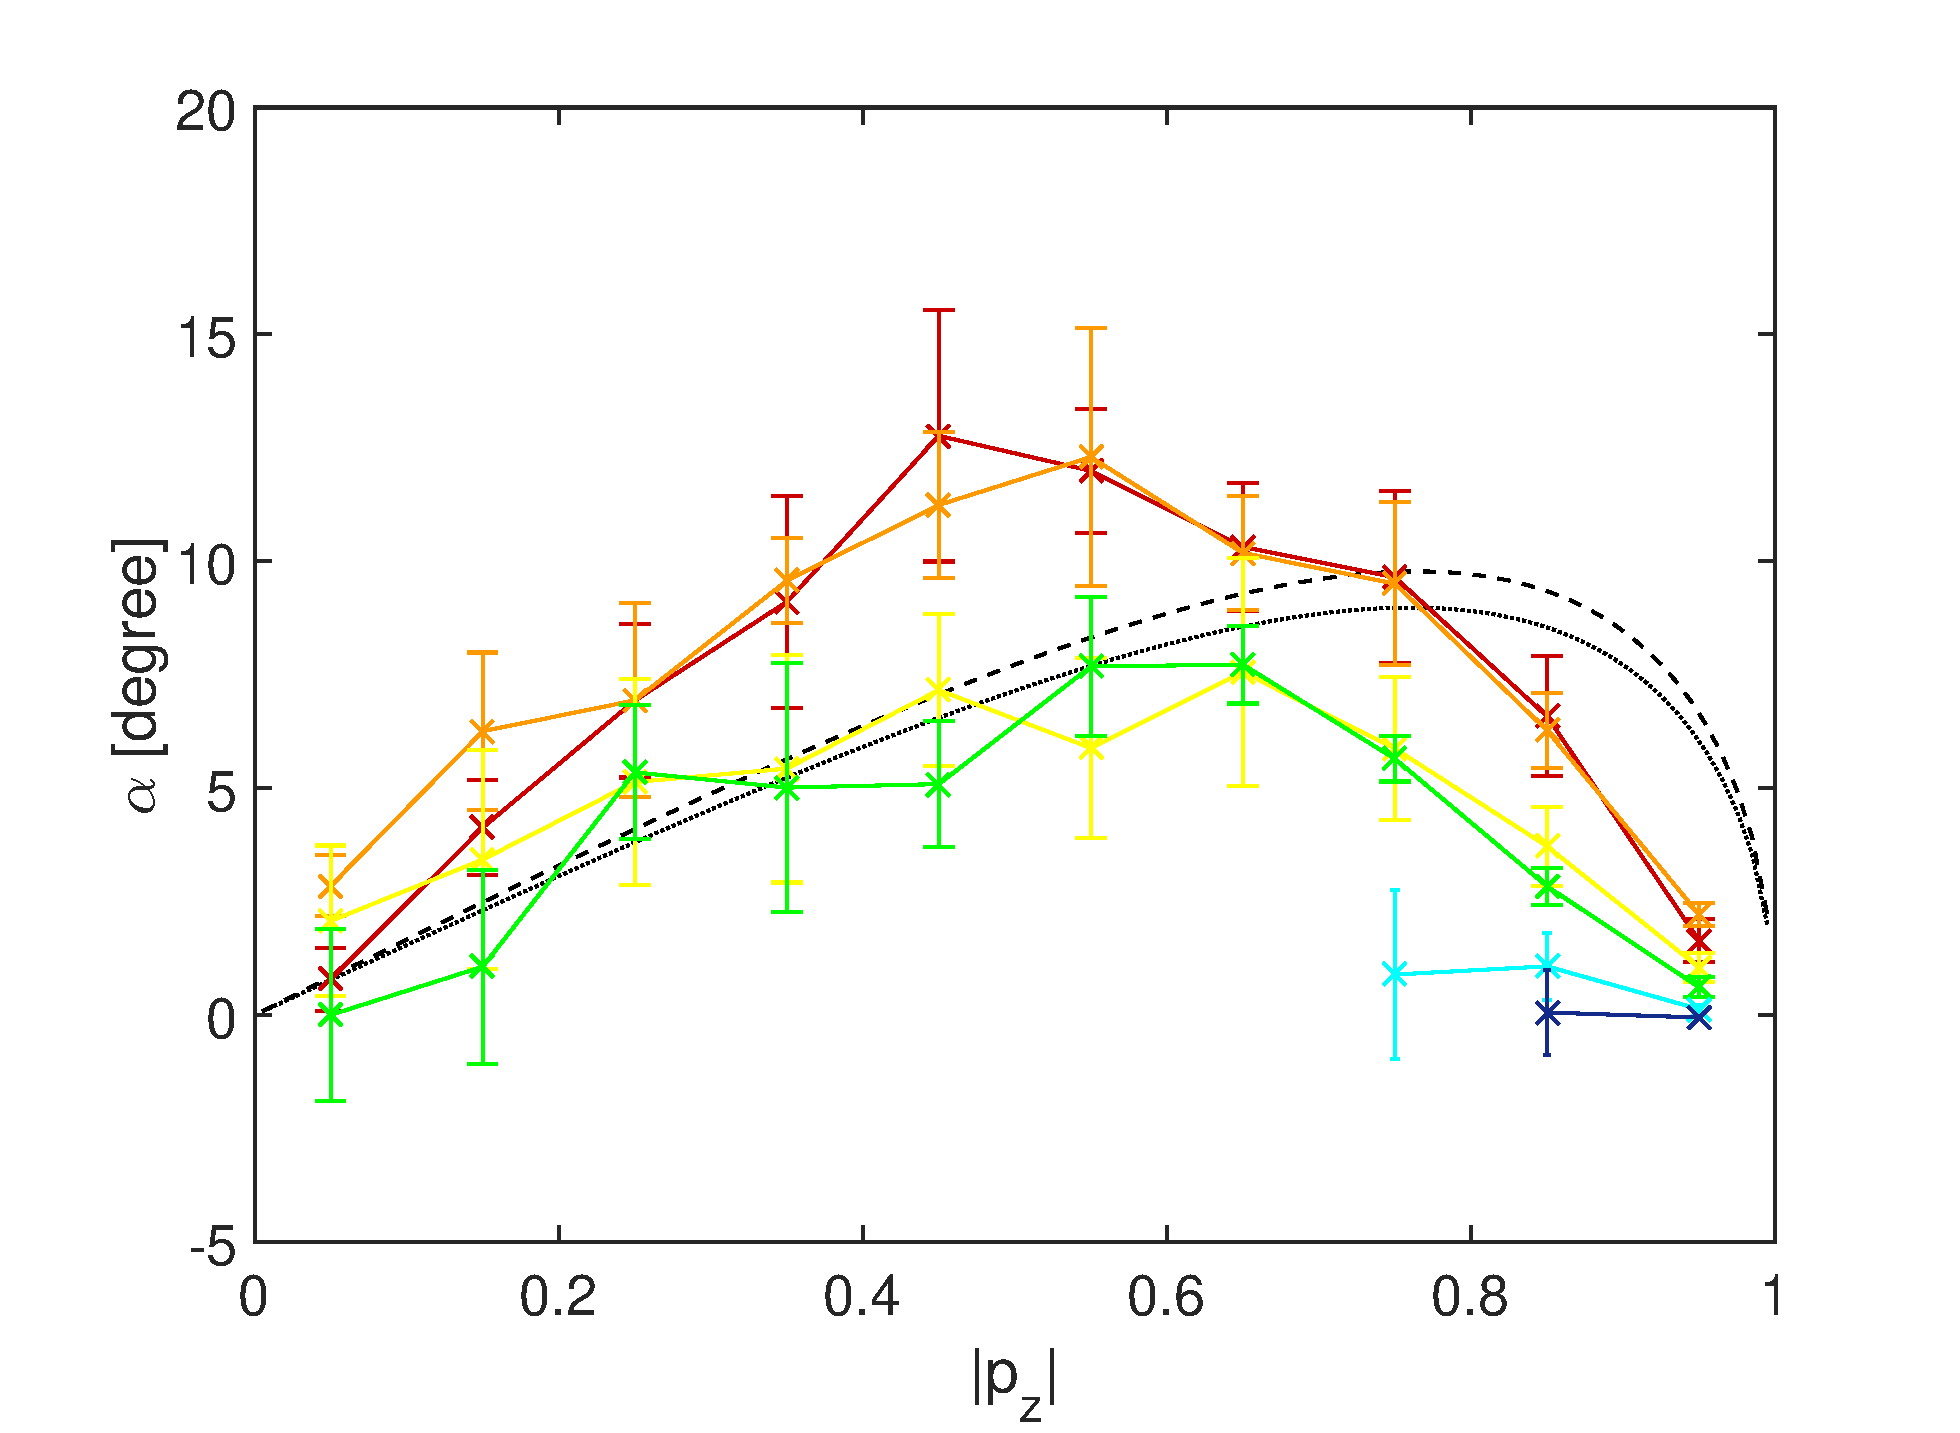
\includegraphics[width=2.9in]{figures/alpha-U-small.pdf}
\end{minipage}
\caption{Angle $\alpha$ between the relative particle velocity and $\mathbf{g}$ for small particles. Left: $\mathbf{w}=(\mathbf{u}_p-\mathbf{u}_f)$ as function of $p_z$. Right: $\mathbf{W}=(\mathbf{u}_p-\mathbf{U}_f)$ as function of $p_z$. Symbols are the same as in Fig.~\ref{Fig:wz}.}
\label{Fig:alpha}
\end{figure}

\begin{figure}
\centering
\begin{minipage}{.5\textwidth}
  \centering
  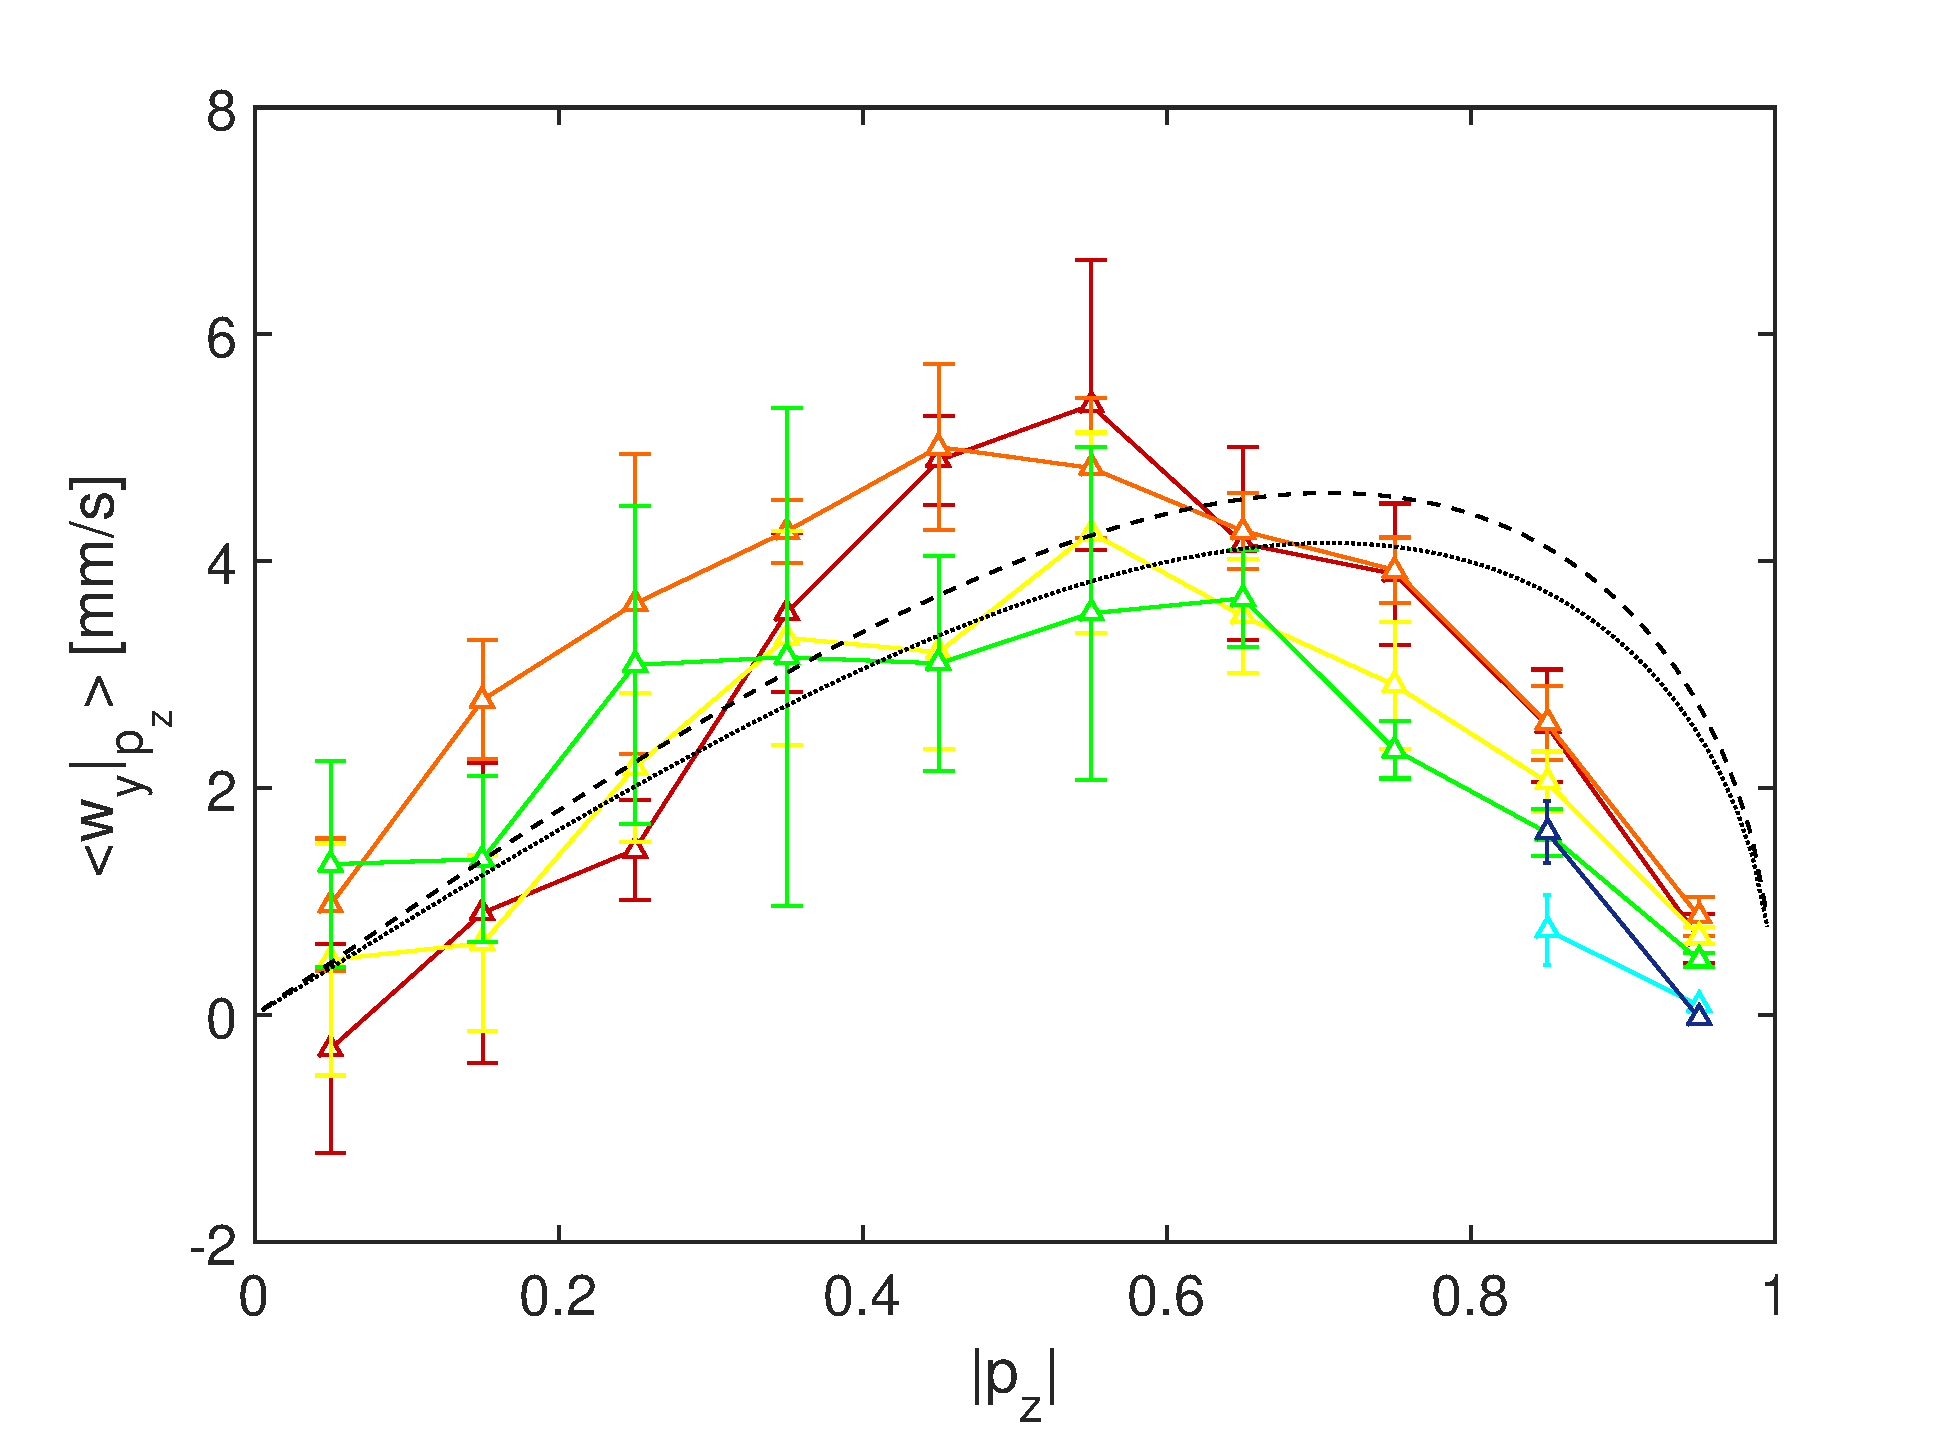
\includegraphics[width=2.9in]{figures/wy-local-small.pdf}
\end{minipage}%
\begin{minipage}{.5\textwidth}
  \centering
  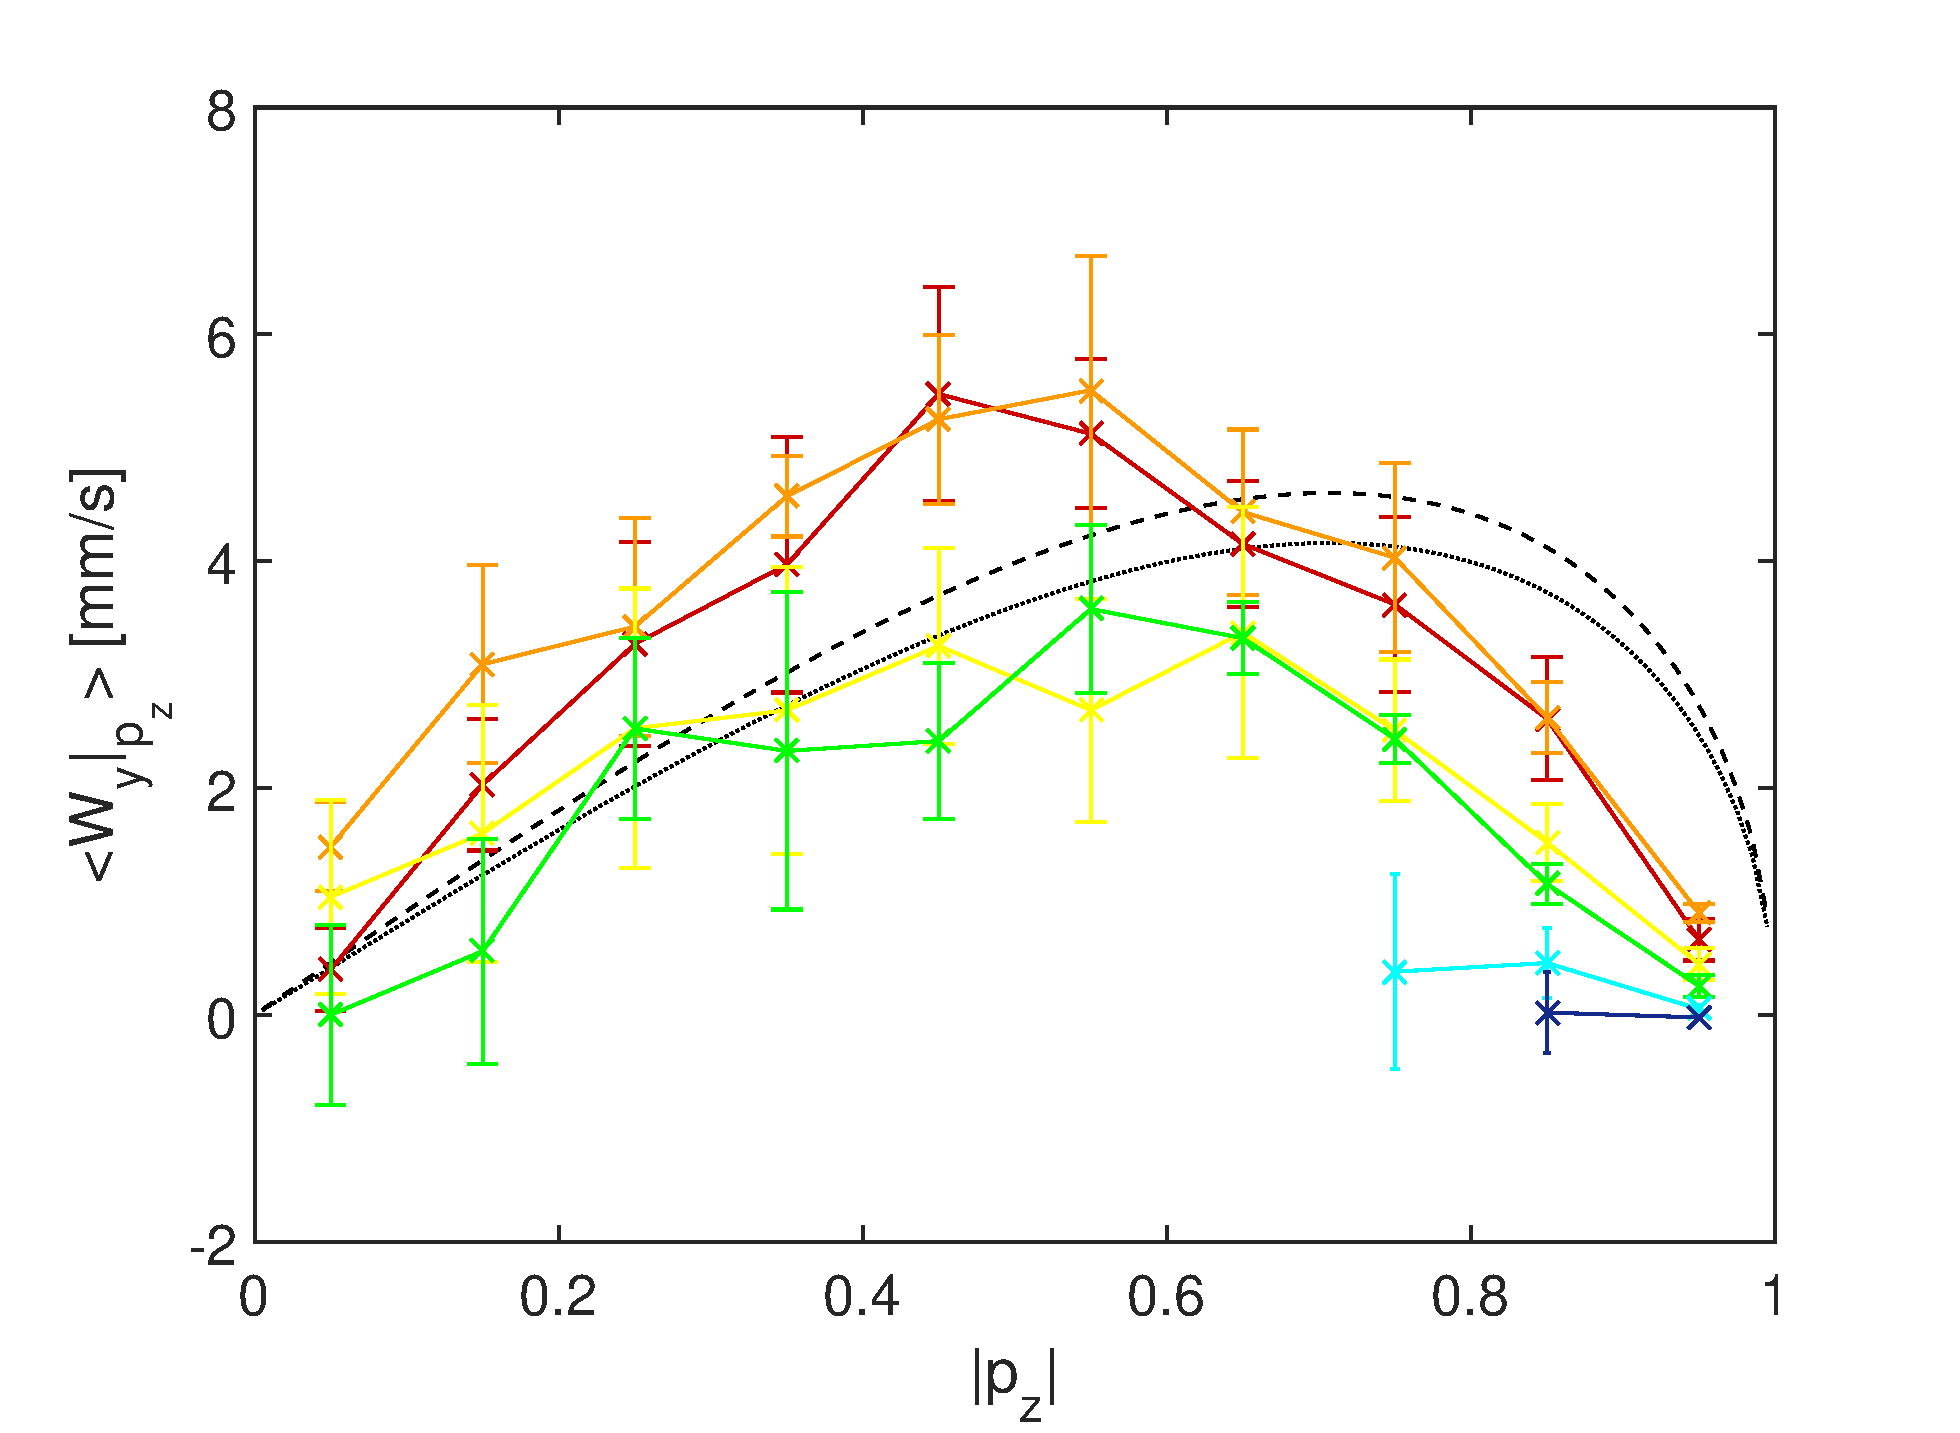
\includegraphics[width=2.9in]{figures/wy-U-small.pdf}
\end{minipage}
\caption{Mean component of the relative particle velocity in $\hat{y}$ direction, conditioned on $|p_z|$ for small particles. Left: $\mathbf{w}=(\mathbf{u}_p-\mathbf{u}_f)$ as function of $p_z$. Right: $\mathbf{W}=(\mathbf{u}_p-\mathbf{U}_f)$ as function of $p_z$. Symbols are the same as in Fig.~\ref{Fig:wz}.}
\label{Fig:wy}
\end{figure}

\begin{figure}
\centering
\begin{minipage}{.5\textwidth}
  \centering
  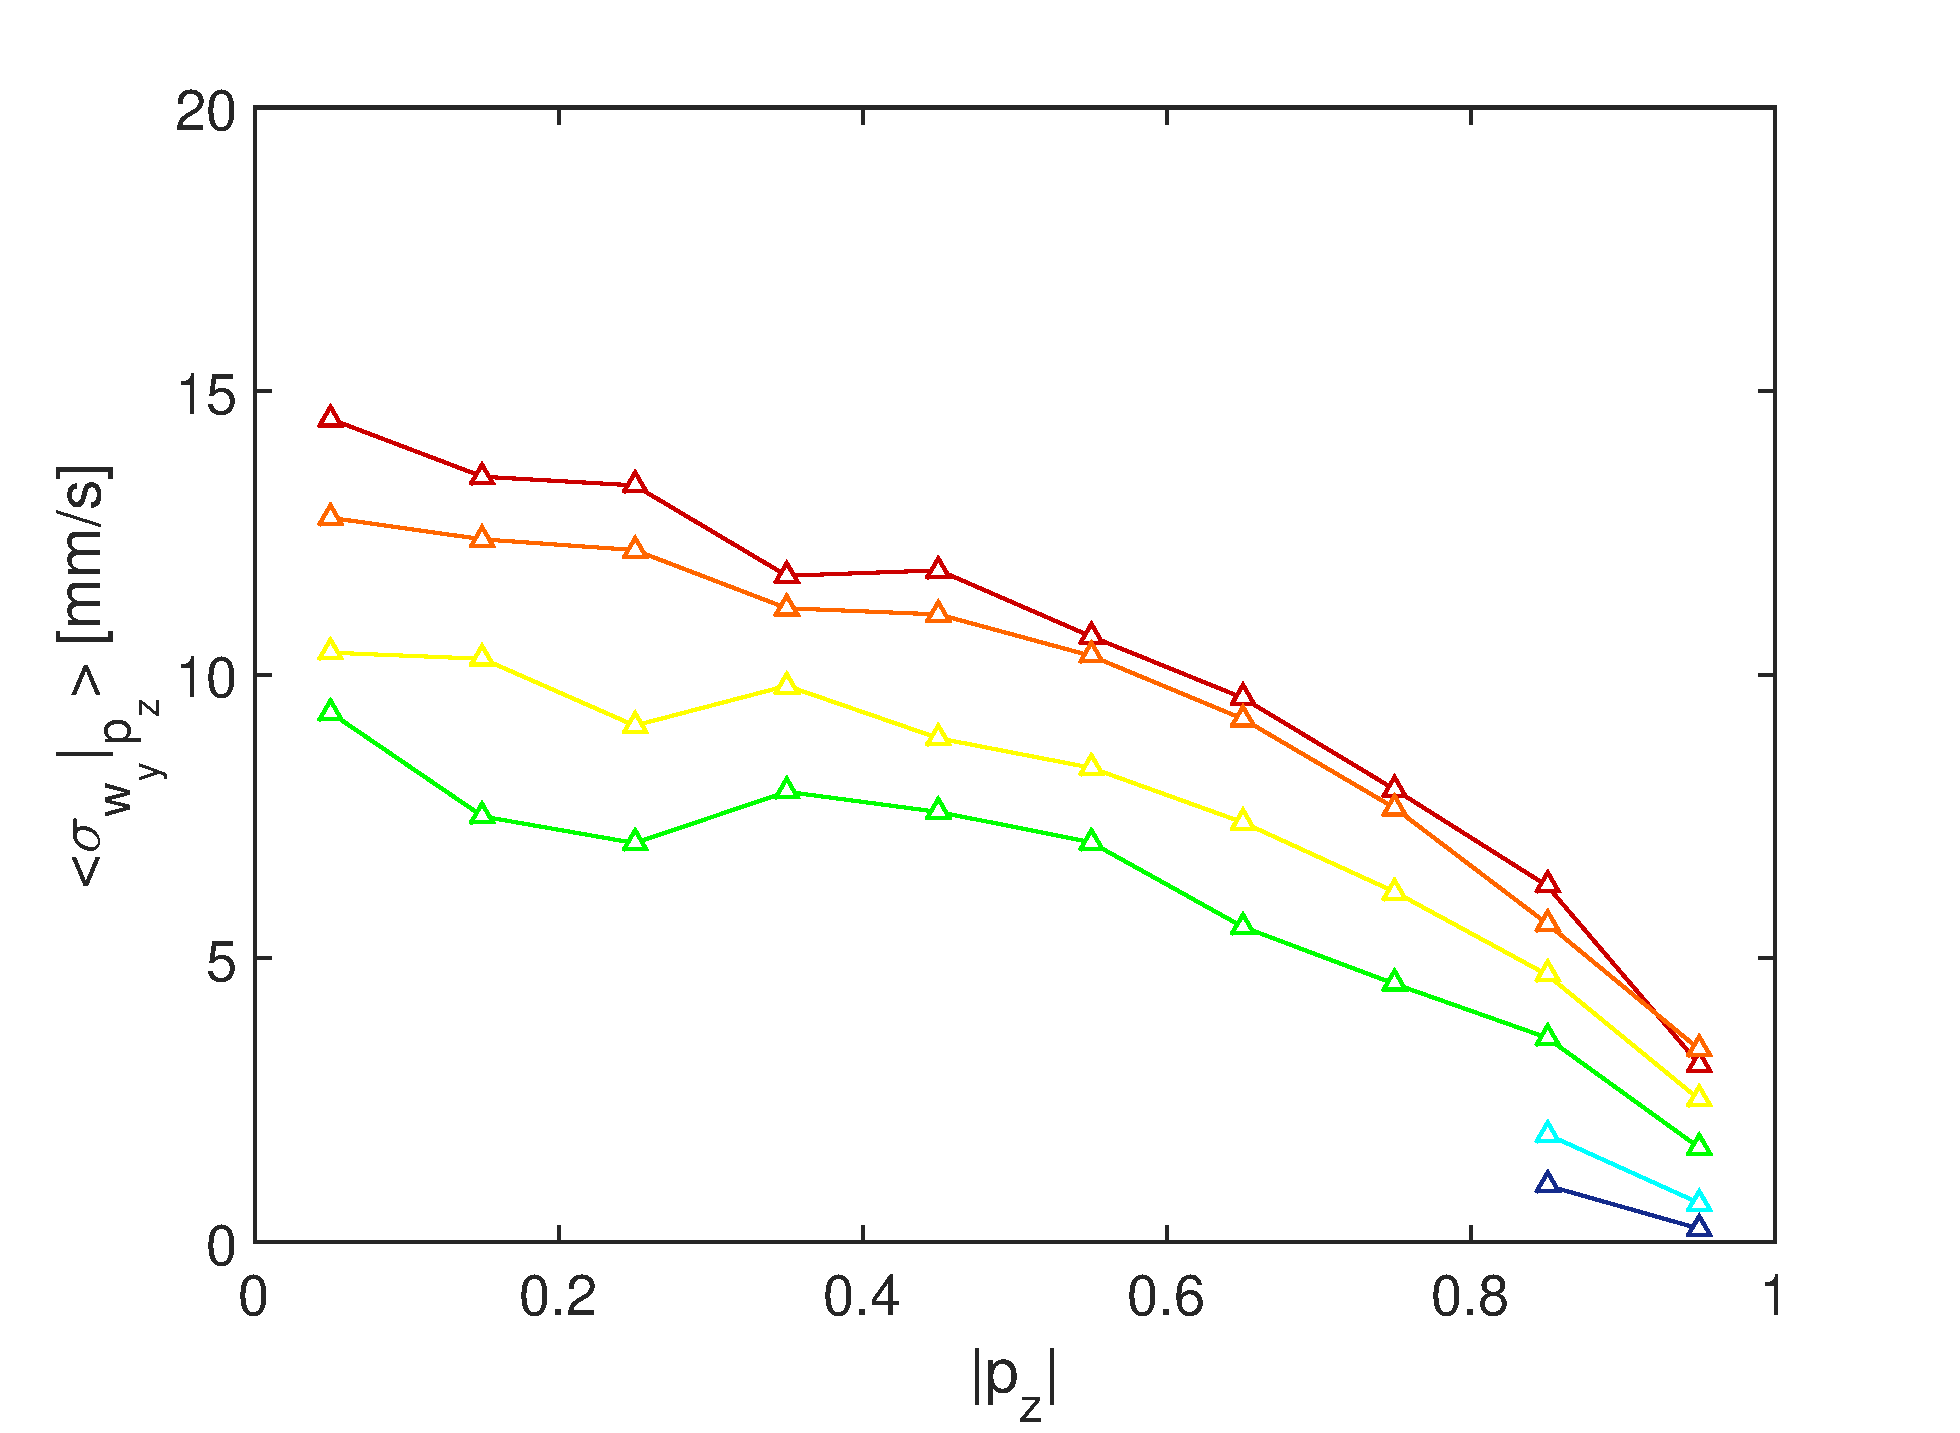
\includegraphics[width=2.9in]{figures/wy-local-sigma-small.pdf}
\end{minipage}%
\begin{minipage}{.5\textwidth}
  \centering
  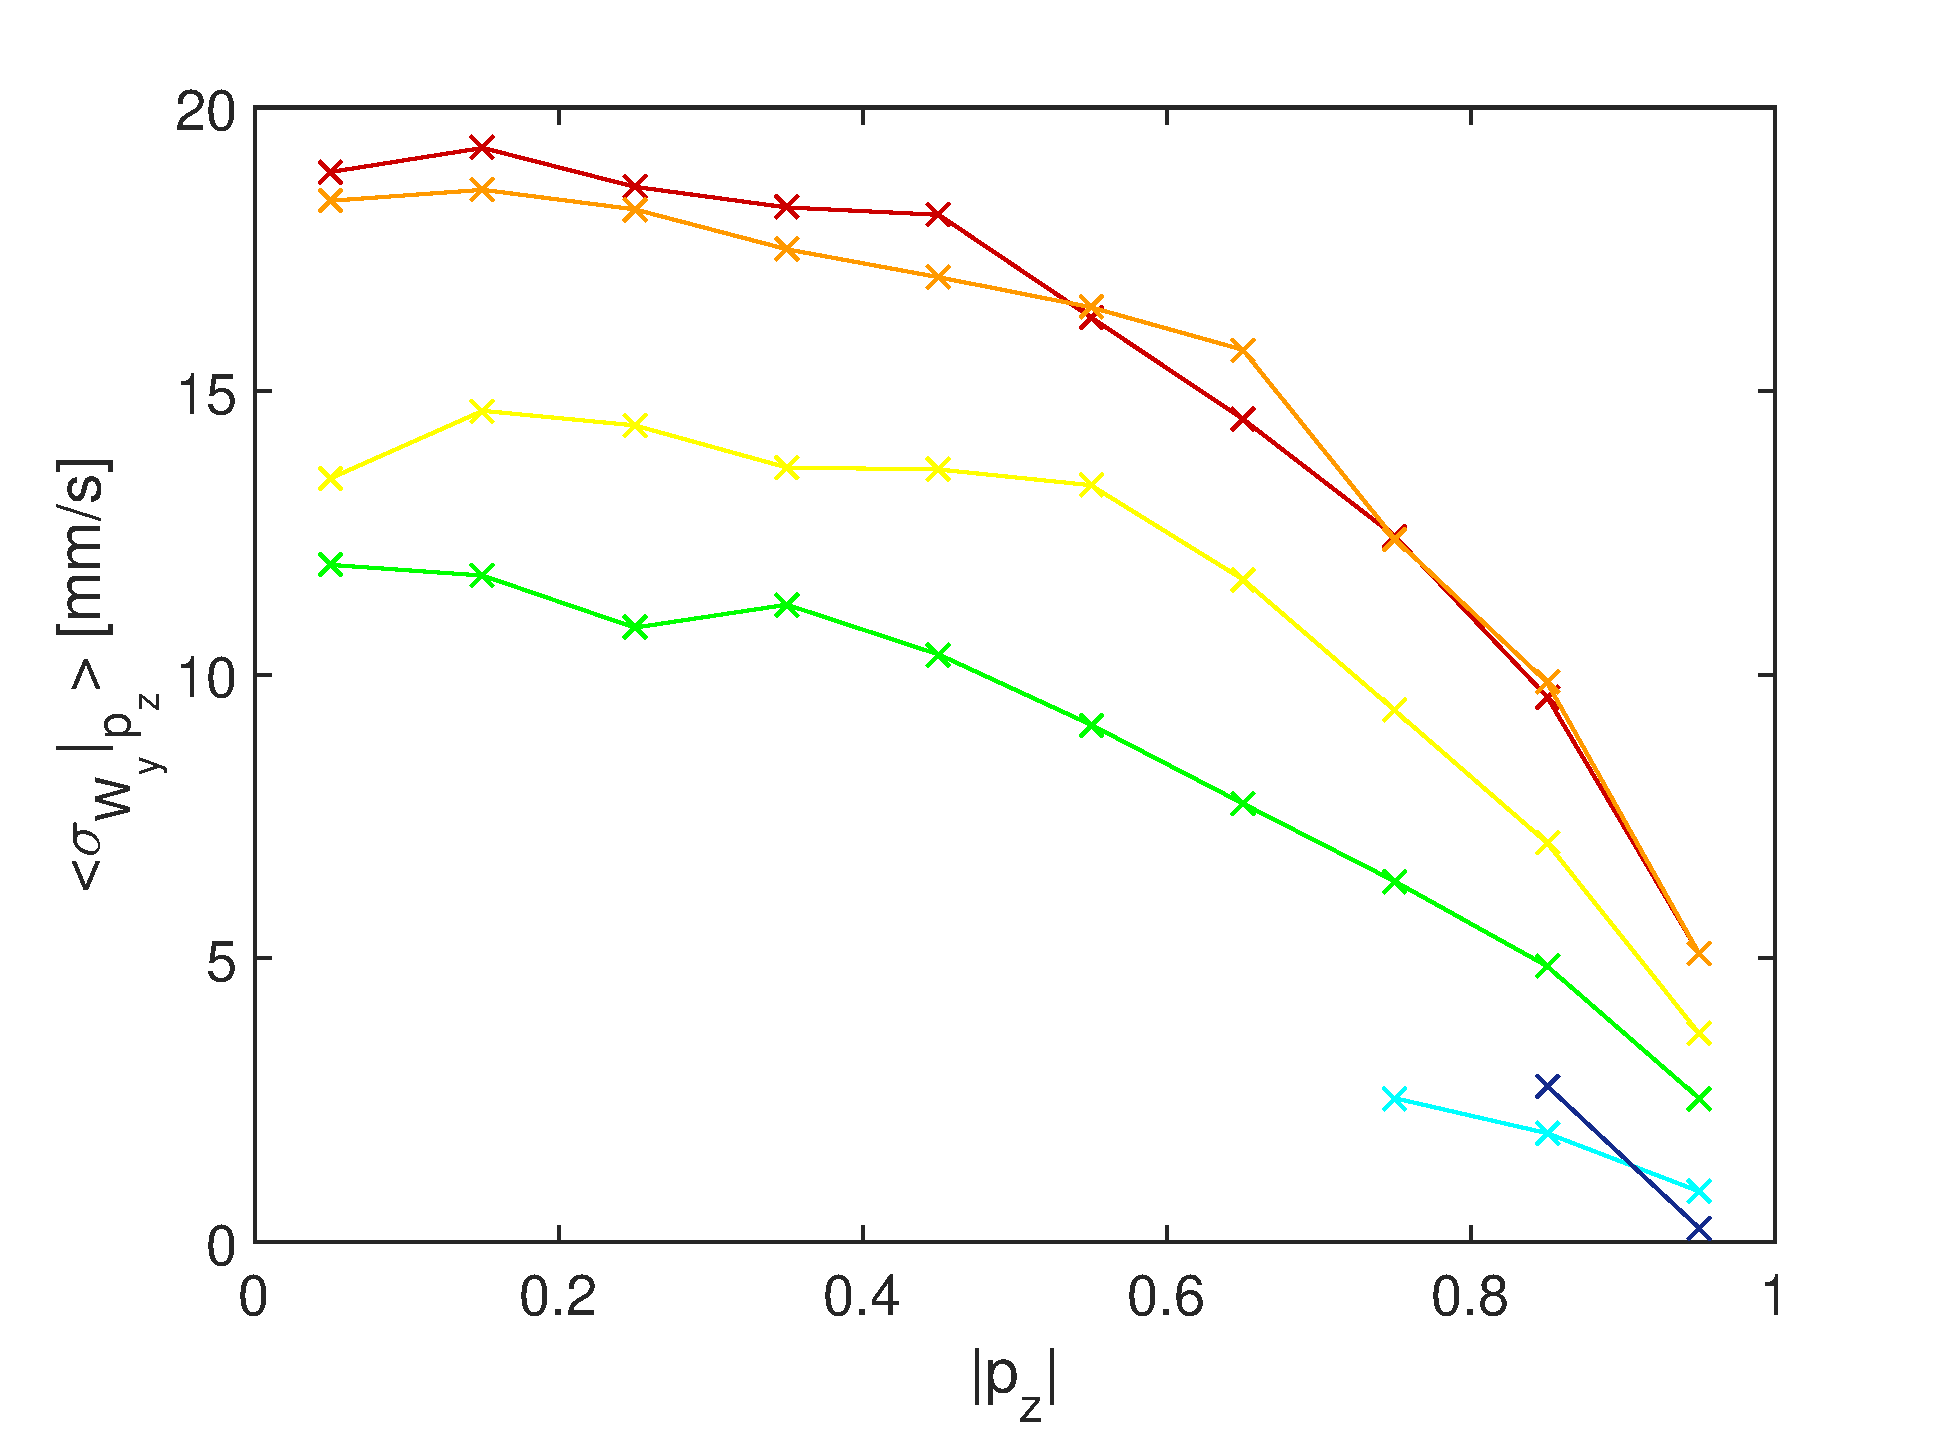
\includegraphics[width=2.9in]{figures/wy-U-sigma-small.pdf}
\end{minipage}
\caption{Standard deviation of the y-component of the relative particle velocity, conditioned on $|p_z|$ for small particles. Left: $\sigma_y=(\langle w_y^2 \rangle-\langle w_y \rangle^2)^{\frac{1}{2}}$. Right: $\sigma_y=(\langle W_y^2 \rangle-\langle W_y \rangle^2)^{\frac{1}{2}}$.}
\label{Fig:wy-sigma}
\end{figure}

\begin{figure}
\centering
\begin{minipage}{.5\textwidth}
  \centering
  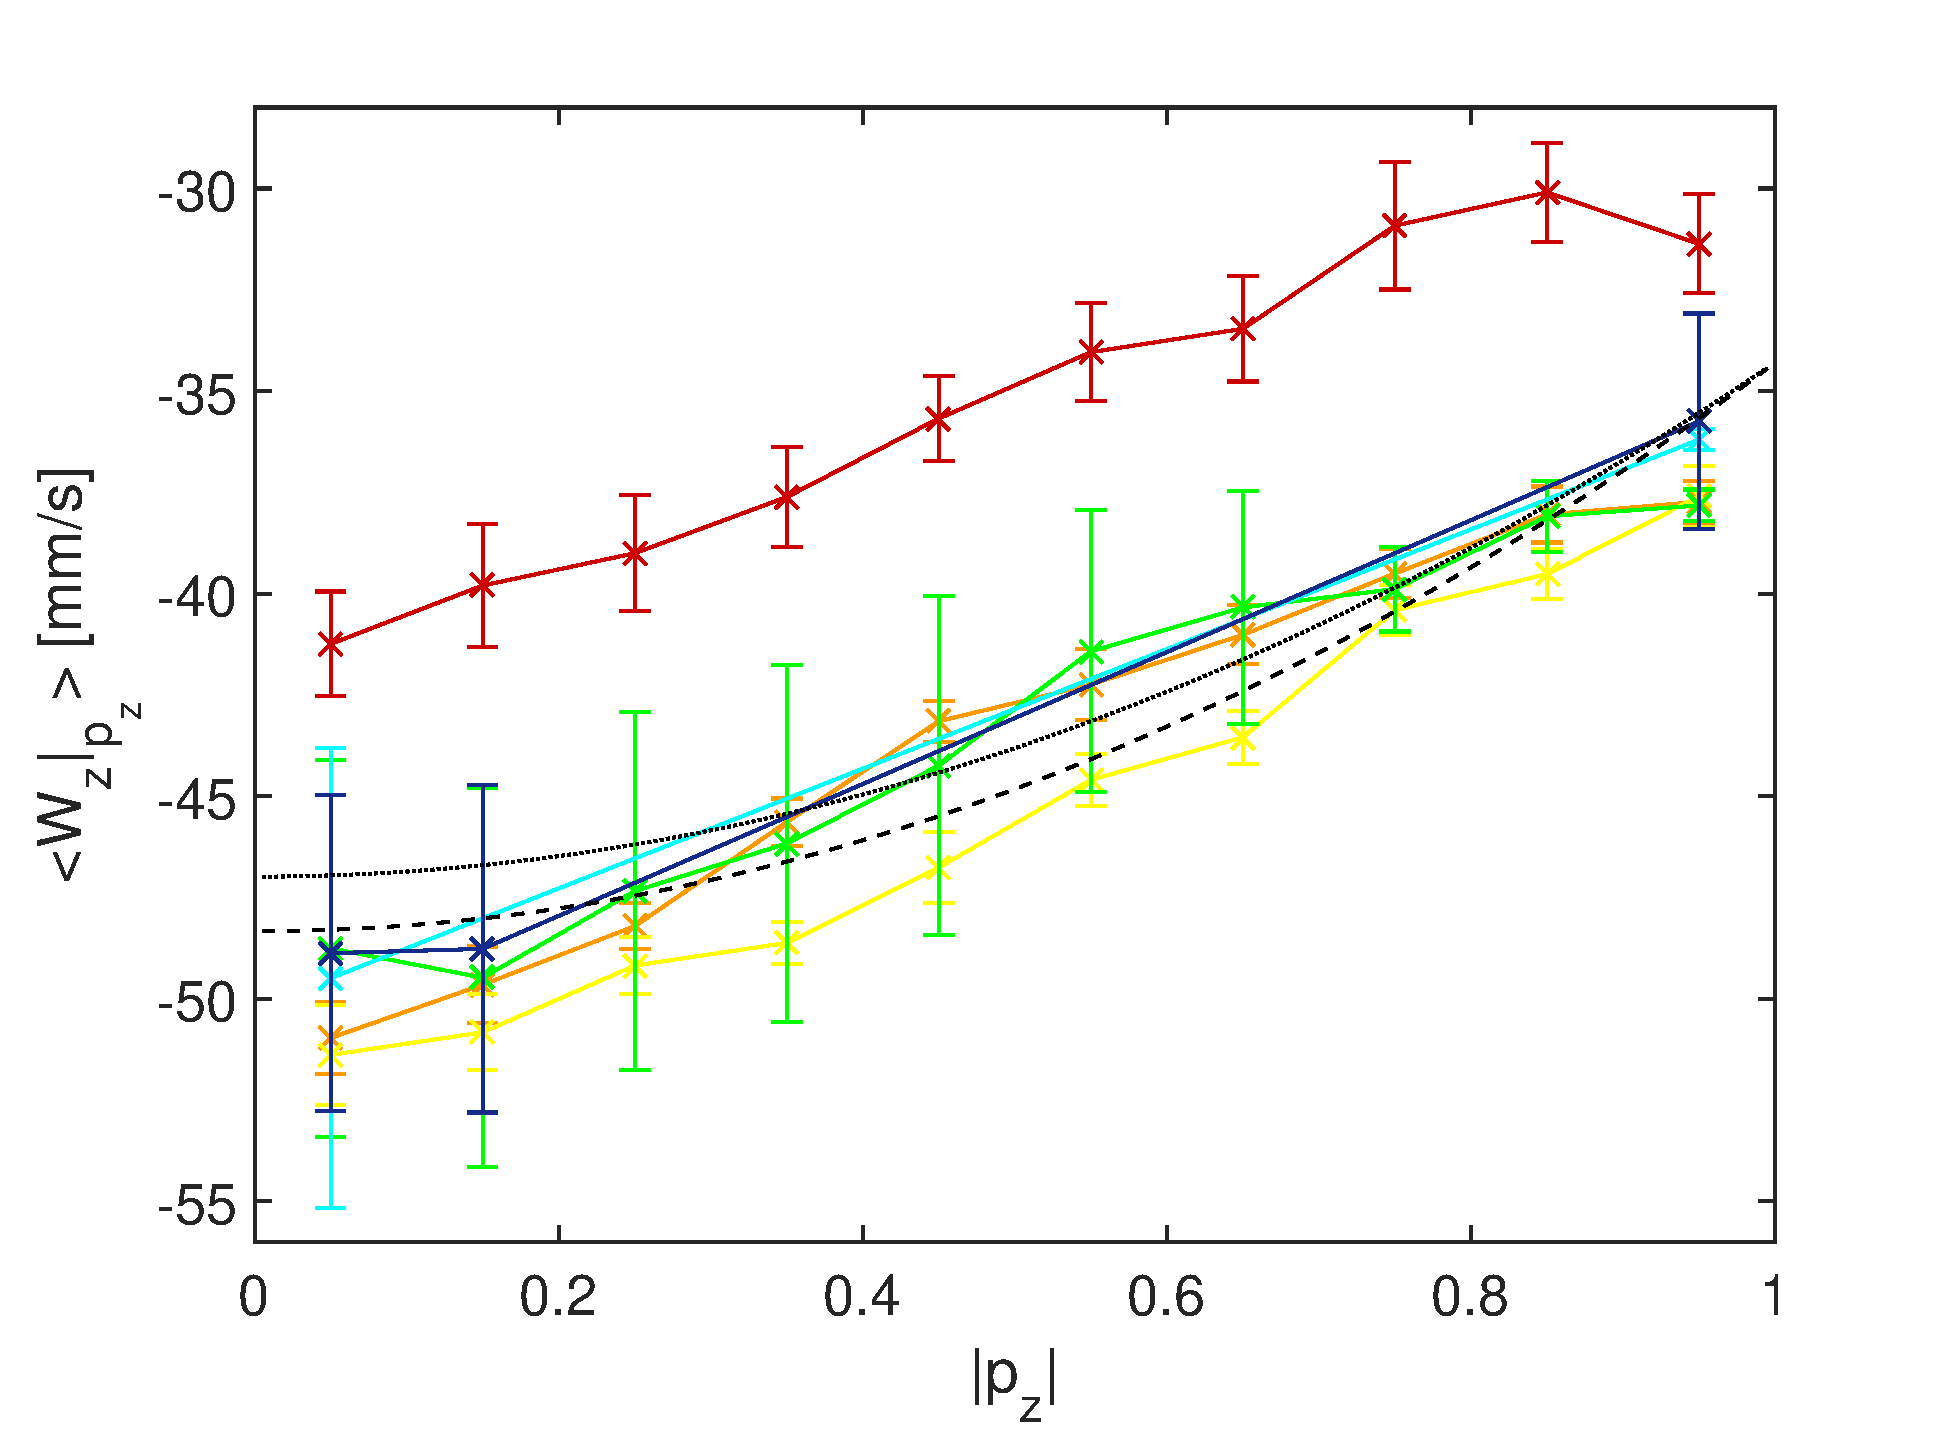
\includegraphics[width=2.9in]{figures/wz-U-large.pdf}
\end{minipage}%
\begin{minipage}{.5\textwidth}
  \centering
  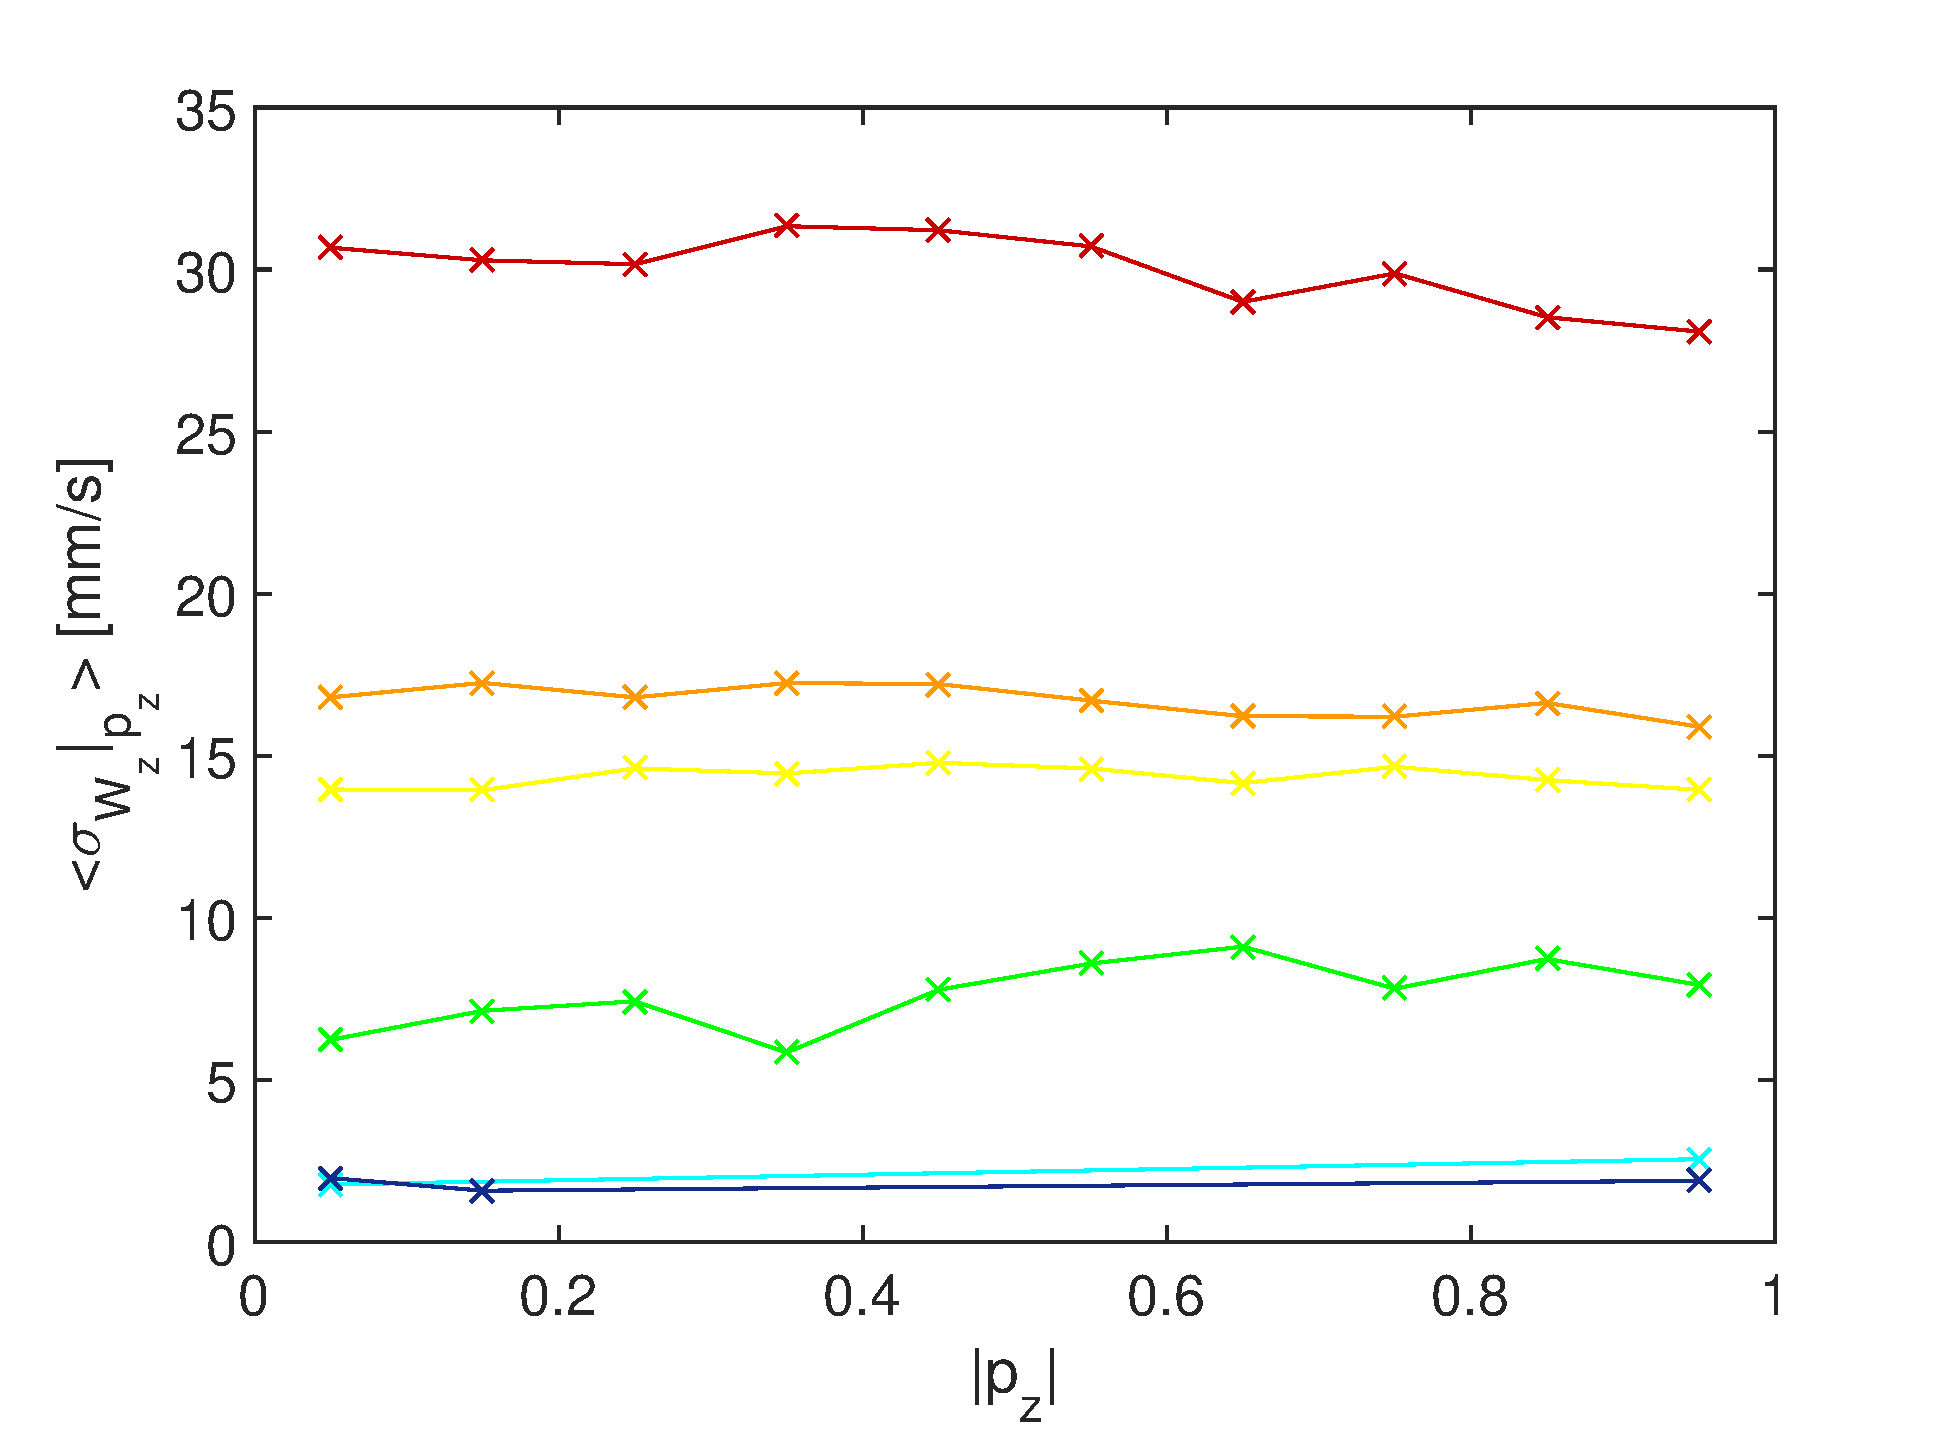
\includegraphics[width=2.9in]{figures/wz-U-sigma-large.pdf}
\end{minipage}
\caption{Left: Mean z-component of the relative particle velocity, conditioned on $|p_z|$ for large particles. Symbols are the same as in Fig.~\ref{Fig:wz}. Right: Standard deviation of the z-component of the relative particle velocity, conditioned on $|p_z|$.}
\label{Fig:wz-large}
\end{figure}

\begin{figure}
\centering
  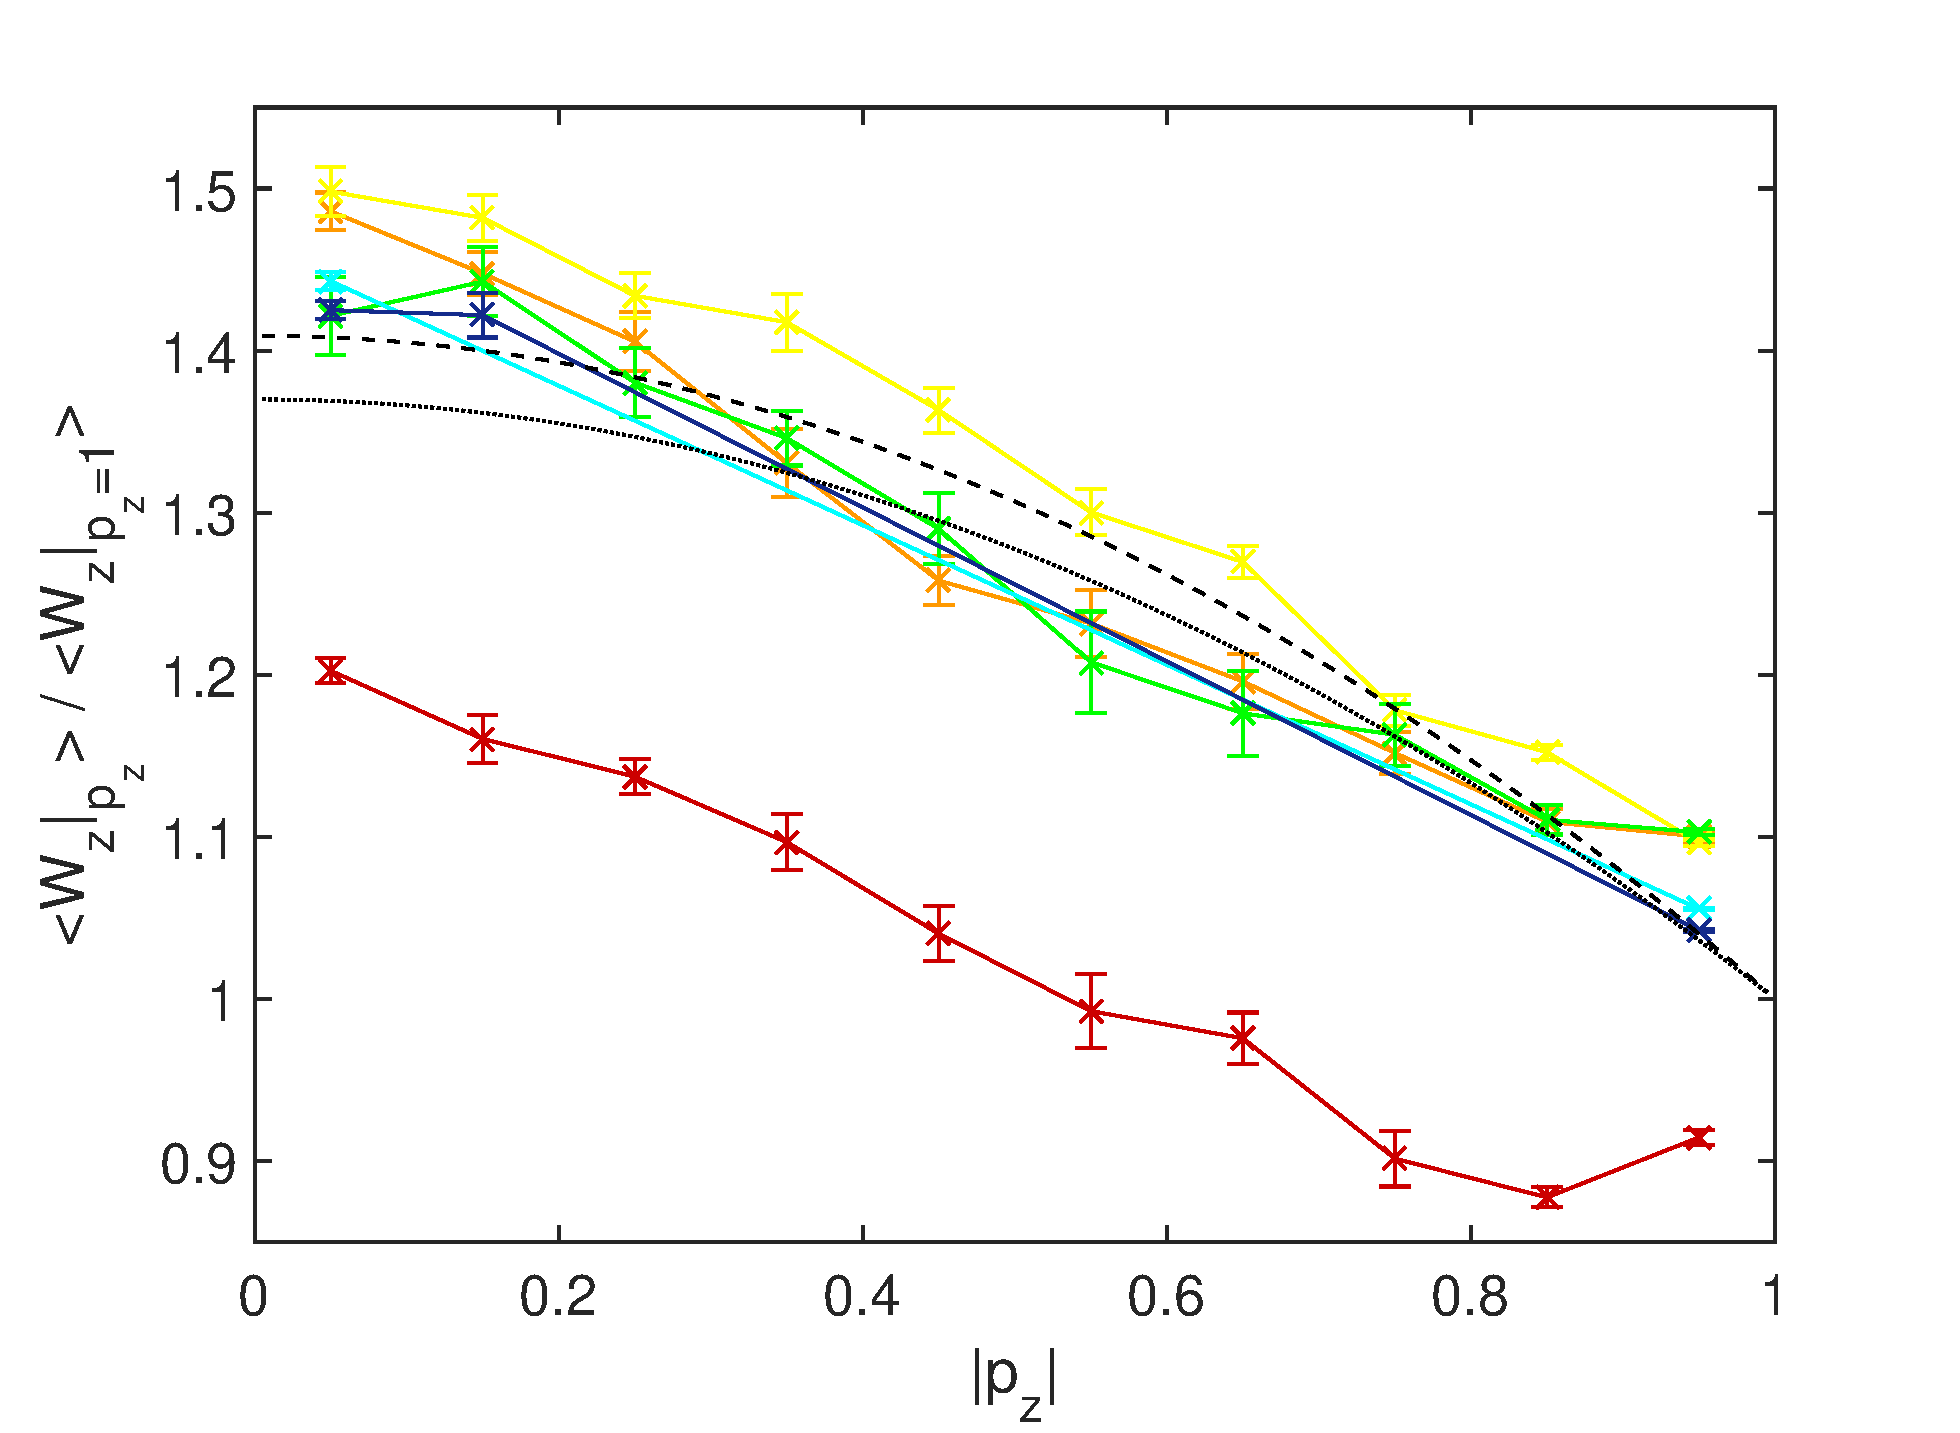
\includegraphics[width=2.9in]{figures/wz-U-norm-large.pdf}
\caption{Mean z-component of the relative particle velocity, conditioned on $|p_z|$, normalized by the particle velocity in quiescent fluid (for large particles). Symbols are the same as in Fig.~\ref{Fig:wz}.}
\label{Fig:wz-norm-large}
\end{figure}

\clearpage

\appendix
\begin{figure}
\centering
  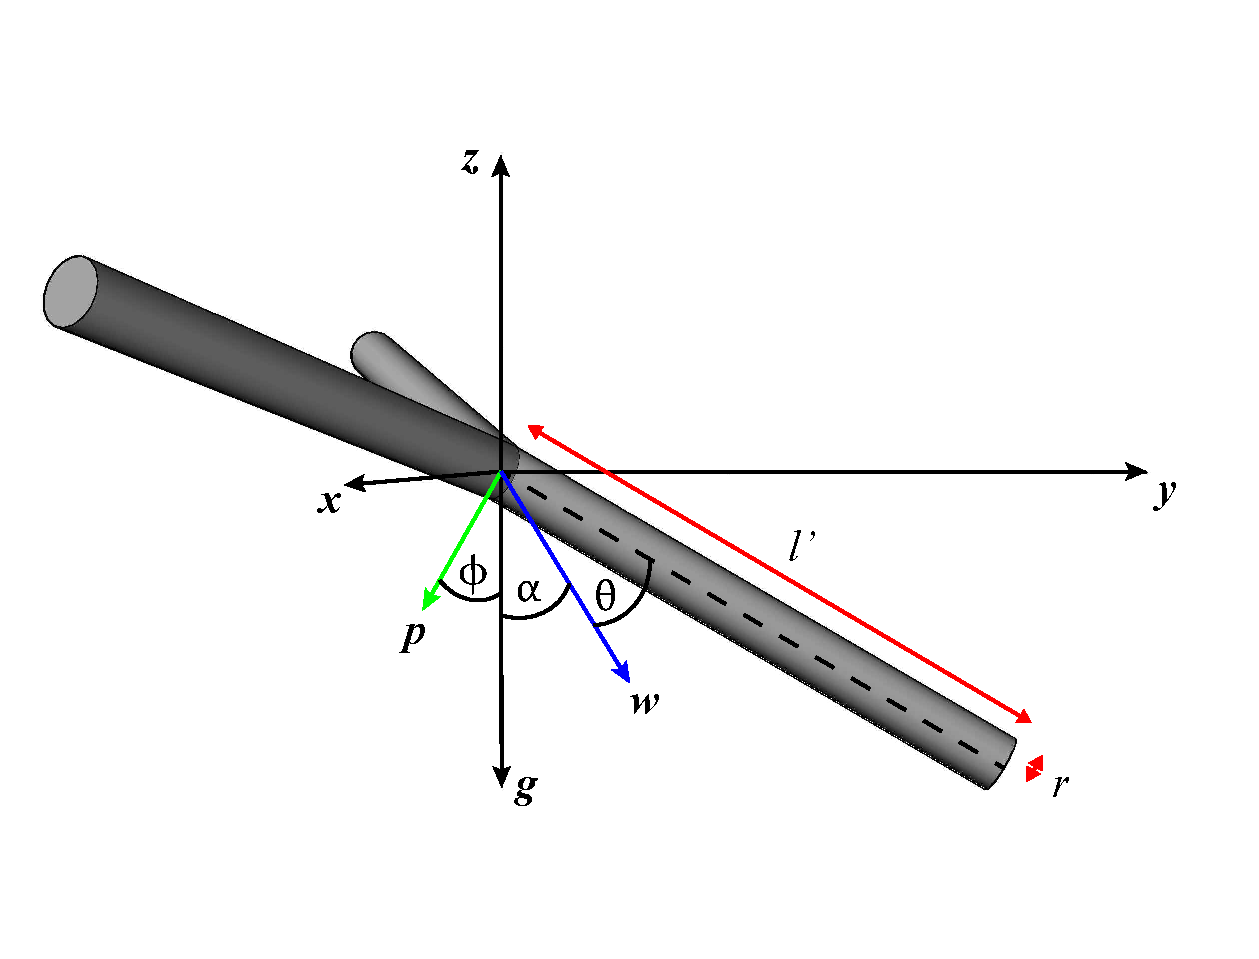
\includegraphics[width=3.2in]{figures/triad-perspective-coord.pdf}
  \caption{Sketch of the coordinate system and variables.}
\label{Fig:triad}
\end{figure}
\section{Coordinate System and Variables}
In three dimensions, $\hat{z}$ points upwards and gravity $\hat{g}$ points downwards (negative $\hat{z}$). The orientation of a particle is described by $\hat{p}$, which is along the symmetry axis of the ellipsoid (horizontally aligned fibers (disks) have $p_z {=} 0$ ($p_z {=} 1$) and vertically aligned fibers (disks) have $p_z {=} 1$ ($p_z {=} 0$)). $\hat{x}$ is perpendicular to the plane spanned by $\hat{p}$ and $\hat{z}$ ($\hat{x}=\hat{p}\times\hat{z}$) and $\hat{y}$ lies in the plane of $\hat{p}$ and $\hat{z}$. The particle velocity is denoted with $\mathbf{u}_p$, the mean fluid velocity at the particle position is $\mathbf{u}_f$ and the mean fluid velocity at infinity is $\mathbf{U}_f$. Therefore, the relative local particle velocity is $\mathbf{w}=\mathbf{u}_p-\mathbf{u}_f$ and the relative particle velocity with respect to infinity is $\mathbf{W}=\mathbf{u}_p-\mathbf{U}_f$. The angle between $\hat{g}$ and $\hat{p}$ is $\phi$, the angle between $\hat{g}$ and $\mathbf{w}$ is $\alpha$ and $\theta=\frac{\pi}{2}-\phi-\alpha$ is the angle between $\mathbf{w}$ and $\hat{p}$. There is one more degree of freedom for triads, which is the orientation of the arms in the plane of the disks, described by the angle $\psi$ around $\hat{p}$. (see Fig.~\ref{Fig:triad} for details)

\section{Theoretical Model}
A simple model for anisotropic particle motion can be obtained by treating the particles as composites of several slender fibers connected at the center which we call a ramified particle. If we neglect the effects of interactions between the fibers, the velocity $\mathbf{W}$ of these sedimenting fibers can be calculated from 
\begin{equation}
W_{i} = M_{ij}F_{j}
\end{equation}
with
\begin{equation}
M_{ij} = M_{\parallel}p_{i}p_{j} + M_{\perp}(\delta_{ij}-p_{i}p_{j})
\end{equation}
\\
where F is the external force on the particle and M the mobility matrix. For infinitely thin fibers at low Reynolds number ($\textit{Re}_l\ll1$), $M_{\parallel} = 2M_{\perp}$.
Here, $M_{\parallel}$ and $M_{\perp}$ is the mobility of the particle along and perpendicular to $\hat{p}$, respectively. For our particles at $\textit{Re}_l=220$, the low Reynolds number approximation is not valid and so we model these effects by allowing the ratio between $M_{\parallel}$ and $M_{\perp}$ to be a fit parameter. 

A disk can either be modeled with two perpendicular fibers (cross) of equal length or three fibers in a plane with a $120^{\circ}$ angle between them (triad). The orientation of the fibers in the plane of the disk does not affect the sedimentation statistics in this simple model. This enables us to calculate the sedimentation velocity as function of particle orientation as shown in Fig.~\ref{Fig:particle-velocity}. 

A spherical particle can be modeled with three, mutually perpendicular fibers and by adjusting the length of individual fibers, we can investigate the aspect ratio dependence of the sedimention velocity of anisotropic particles. In Fig.~\ref{Fig:particle-velocity}, the red crosses and blue triangles show the vertical and horizontal components of the sedimentation velocity of fibers and disks, respectively. The dashed (dotted) lines show how fibers (disks) approach the spherical case.  Fibers sediment 2 times faster when $p_z{=}1$ compared to $p_z{=}0$, whereas disks sediment 1.5 times faster when $p_z{=}0$ compared to $p_z{=}1$.

From experimental measurements in quiescent fluid, we know the sedimentation rate of triads for $p_z{=}0$ and $p_z{=}1$ (these are the same as shown Fig.~\ref{Fig:wz-norm}). We can normalize the sedimentation velocity of our model disk with these values and compare it to the measurements. In the figures above, the black dashed line shows the theoretical prediction using $M_{\parallel} = 2M_{\perp}$ for each fiber of the model. The black dotted line shows the theoretical prediction using $M_{\parallel} = 1.9M_{\perp}$ for each fiber of the model.

\section{Tables}
\begin{table}
  \begin{center}
\def~{\hphantom{0}}
  \begin{tabular}{ccccccccc} 
	Small particles \\
	\hline
			Turb. Int. & $\langle U_{f} \rangle$ & $u'_{(x,y,z)}/u'_z$ & $\textit{Re}_{\lambda}$ & $\bar{u}$ & $L$ & $\epsilon$ & $\eta$ & $\tau_{\eta}$ \\[3pt]
			0.08 & 19.78 & 0.83 0.90 1.00 & ~34 & 1.38 & ~52 & 0.05 & 1.98 & 4.33 \\
			0.23 & 23.39 & 0.79 0.79 1.00 & ~95 & 4.52 & 123 & 0.75 & 1.00 & 1.12 \\
			0.39 & 29.85 & 0.85 0.85 1.00 & 141 & 10.34 & 116 & 9.5 & 0.53 & 0.31 \\
			0.62 & 26.91 & 0.83 0.83 1.00 & 162 & 14.80 & 108 & 30 & 0.39 & 0.18 \\
			0.91 & 21.96 & 0.87 0.87 1.00 & 192 & 18.31 & 123 & 50 & 0.35 & 0.14 \\
			1.06 & 20.08 & 0.85 0.86 1.00 & 194 & 19.25 & 119 & 60 & 0.33 & 0.13 \\
			\hline
	Large particles \\
	\hline
			Turb. Int. & $\langle U_{f} \rangle$ & $u'_{(x,y,z)}/u'_z$ & $\textit{Re}_{\lambda}$ & $\bar{u}$ & $L$ & $\epsilon$ & $\eta$ & $\tau_{\eta}$ \\[3pt]
			0.07 & 34.14 & 0.78 0.79 1.00 & ~35 & 2.16 & ~34 & 0.3 & 1.26 & 1.77 \\
			0.10 & 30.63 & 0.82 0.80 1.00 & ~56 & 2.74 & ~69 & 0.3 & 1.26 & 1.77 \\
			0.29 & 31.68 & 0.86 0.86 1.00 & 102 & 8.32 & ~77 & 7.5 & 0.56 & 0.35 \\
			0.28 & 58.00 & 0.85 0.85 1.00 & 153 & 14.39 & 99 & 30 & 0.40 & 0.17 \\
			0.37 & 50.29 & 0.86 0.84 1.00 & 162 & 16.83 & 95 & 50 & 0.35 & 0.14 \\
			0.95 & 30.06 & 0.86 0.85 1.00 & 200 & 25.75 & 95 & 180 & 0.25 & 0.07 \\
  \end{tabular}
  \caption{Turbulence parameters for small triads.  $u'_z/\langle U_f \rangle$, turbulence intensity in the direction of the mean fluid flow $\langle U_f \rangle$; $u'_{(x,y,z)}$, rms fluctuating velocity components [mm/s];  $\textit{Re}_{\lambda}=\sqrt{15\bar{u}L/\nu}$, Reynolds number;  $\bar{u}=\langle u'_i \rangle_i$, fluctuating velocity [mm/s];  $L=\bar{u}^3/\epsilon$, energy input length scale [mm];  $\epsilon$, energy dissipation rate [mm$^2$/s$^3$];  $\eta=(\nu^3/\epsilon)^{1/4}$, Kolmogorov length [mm];  $\tau_{\eta}=(\nu/\epsilon)^{1/2}$, Kolmogorov time [s];}
  \label{tab:kd1}
  \end{center}
\end{table}

\newpage

\bibliographystyle{jfm}
% Note the spaces between the initials
%\nocite{*}
\bibliography{orientation-sedimentation-bib}

\end{document}
